\PassOptionsToPackage{hyphens}{url}
\documentclass[11pt]{article}
\usepackage[T1]{fontenc}
\usepackage[utf8]{inputenc}
\usepackage{lmodern}
\input{glyphtounicode}
\pdfglyphtounicode{angbracketleftBigg}{27E8}
\pdfglyphtounicode{angbracketleftbig}{27E8}
\pdfglyphtounicode{angbracketrightBigg}{27E9}
\pdfglyphtounicode{angbracketrightbig}{27E9}
\pdfglyphtounicode{arrowhookleft}{02D3}
\pdfglyphtounicode{braceex}{23AA}
\pdfglyphtounicode{braceleftbigg}{007B}
\pdfglyphtounicode{braceleftbt}{23A9}
\pdfglyphtounicode{braceleftmid}{23A8}
\pdfglyphtounicode{bracelefttp}{23A7}
\pdfglyphtounicode{bracerightbigg}{007D}
\pdfglyphtounicode{bracketleftbig}{005B}
\pdfglyphtounicode{bracketleftbigg}{005B}
\pdfglyphtounicode{bracketleftbt}{23A3}
\pdfglyphtounicode{bracketlefttp}{23A1}
\pdfglyphtounicode{bracketrightbig}{005D}
\pdfglyphtounicode{bracketrightbigg}{005D}
\pdfglyphtounicode{bracketrightbt}{23A6}
\pdfglyphtounicode{bracketrighttp}{23A4}
\pdfglyphtounicode{hatwide}{0302}
\pdfglyphtounicode{integraldisplay}{222B}
\pdfglyphtounicode{integraltext}{222B}
\pdfglyphtounicode{intersectiondisplay}{22C2}
\pdfglyphtounicode{intersectiontext}{22C2}
\pdfglyphtounicode{mapsto}{007C}
\pdfglyphtounicode{parenleftBig}{0028}
\pdfglyphtounicode{parenleftBigg}{0028}
\pdfglyphtounicode{parenleftbig}{0028}
\pdfglyphtounicode{parenleftbigg}{0028}
\pdfglyphtounicode{parenleftbt}{239D}
\pdfglyphtounicode{parenlefttp}{239B}
\pdfglyphtounicode{parenrightBig}{0029}
\pdfglyphtounicode{parenrightBigg}{0029}
\pdfglyphtounicode{parenrightbig}{0029}
\pdfglyphtounicode{parenrightbigg}{0029}
\pdfglyphtounicode{parenrightbt}{23A0}
\pdfglyphtounicode{parenrighttp}{239E}
\pdfglyphtounicode{productdisplay}{220F}
\pdfglyphtounicode{producttext}{220F}
\pdfglyphtounicode{radicalbig}{221A}
\pdfglyphtounicode{summationdisplay}{2211}
\pdfglyphtounicode{summationtext}{2211}
\pdfglyphtounicode{uniontext}{22C3}
\pdfglyphtounicode{vextenddouble}{2225}
\pdfglyphtounicode{vextendsingle}{007C}
\pdfgentounicode=1
\usepackage[margin=1in]{geometry}
\usepackage{amsmath,amssymb,amsthm,mathtools,mathrsfs}
\usepackage[expansion=false]{microtype}
\usepackage{enumitem,booktabs,array}
\usepackage{needspace}
\usepackage{graphicx,tikz}
\usetikzlibrary{arrows.meta,calc,patterns,positioning}
\usepackage[unicode,colorlinks=true,linkcolor=blue!45!black,citecolor=blue!45!black,urlcolor=blue!45!black]{hyperref}
\usepackage[capitalise,noabbrev,nameinlink]{cleveref}
\hypersetup{pdftitle={The Gaussian free field limit of integer Lipschitz heights with two-arc boundary data},pdfauthor={OpenAI}}
\numberwithin{equation}{section}
\newtheorem{theorem}{Theorem}[section]
\newtheorem{proposition}[theorem]{Proposition}
\newtheorem{lemma}[theorem]{Lemma}
\newtheorem{corollary}[theorem]{Corollary}
\theoremstyle{definition}
\newtheorem{definition}[theorem]{Definition}
\newtheorem{remark}[theorem]{Remark}
\newcommand{\preserveresulttype}[1]{%
  \AtBeginEnvironment{#1}{\crefalias{theorem}{#1}}}
\forcsvlist{\preserveresulttype}{theorem,proposition,lemma,corollary,definition,remark}
\makeatletter
\newcommand{\reserveresultspace}[1]{%
  \BeforeBeginEnvironment{#1}{%
    \if@nobreak\else\Needspace{4\baselineskip}\fi}}
\makeatother
\forcsvlist{\reserveresultspace}{theorem,proposition,lemma,corollary,definition,remark}
\newcommand{\PP}{\mathbb P}
\newcommand{\EE}{\mathbb E}
\newcommand{\R}{\mathbb R}
\newcommand{\Z}{\mathbb Z}
\newcommand{\N}{\mathbb N}
\newcommand{\C}{\mathbb C}
\newcommand{\Tri}{\mathbb T}
\newcommand{\eps}{\varepsilon}
\newcommand{\one}{\mathbf 1}
\DeclareMathOperator{\Var}{Var}
\DeclareMathOperator{\Cov}{Cov}
\DeclareMathOperator{\dist}{dist}
\DeclareMathOperator{\supp}{supp}
\DeclareMathOperator{\Rea}{Re}
\DeclareMathOperator{\Ima}{Im}
\DeclarePairedDelimiter{\abs}{\lvert}{\rvert}
\DeclarePairedDelimiter{\norm}{\lVert}{\rVert}
\setlist[itemize]{topsep=4pt,itemsep=2pt}
\setlist[enumerate]{topsep=4pt,itemsep=2pt}
\title{The Gaussian free field limit of integer Lipschitz heights with two-arc boundary data}
\author{OpenAI}
\date{September 25, 2026}
\begin{document}
\maketitle
\begin{abstract}
We prove that the centered uniform odd integer height function on triangular-lattice approximations of a smooth simply connected domain, with neighboring differences zero or two and boundary values $+1$ and $-1$ on two arcs, converges to a universal multiple of the Dirichlet Gaussian free field. This resolves the field part of Schramm's Problem~2.2. We give an absolutely convergent finite-volume formula for the normalization. The proof combines reflection positivity, a spectral sum rule, and boundary comparison with Gaussian moment identities.
\end{abstract}
\tableofcontents
\section{Introduction}\label{sec:introduction}

Uniform Lipschitz heights are among the simplest random surface models with a
hard local constraint.  Their planar fluctuations are expected to be governed
by the Gaussian free field.  We prove this for integer heights on the
triangular lattice with the two-arc boundary condition proposed by Schramm.
The conclusion concerns the field, including all joint test-function limits
and distributional tightness.

\subsection{The model and the limit}

Write
\[
 \Tri=\Z(1,0)+\Z(1/2,\sqrt3/2)
\]
for the unit triangular lattice.  Let $D\subset\R^2$ be bounded, smooth, and
simply connected, and let $a,b$ be distinct points of $\partial D$.  They
divide the boundary into open arcs $A_+$ and $A_-$.  For $\delta\downarrow0$,
let $D_\delta$ be simply connected polygonal domains made of triangles of
$\delta\Tri$, whose marked boundary parametrizations converge uniformly to
that of $(D,a,b)$.  Put the discrete marks at the midpoints of distinct
boundary edges.  The boundary vertices then split into disjoint sets
$A_{+,\delta}$ and $A_{-,\delta}$; no vertex receives two prescriptions.

Choose $h_\delta$ uniformly among the odd integer functions on the vertices
of $D_\delta$ satisfying
\begin{equation}\label{eq:odd-model}
 h_\delta=1\text{ on }A_{+,\delta},\qquad
 h_\delta=-1\text{ on }A_{-,\delta},\qquad
 |h_\delta(x)-h_\delta(y)|\in\{0,2\}\quad(x\sim y).
\end{equation}
Extend the function affinely on every triangle.  For a test function
$f\in C_c^\infty(D)$, write $h_\delta(f)=\int h_\delta(x)f(x)\,dx$ once its
support lies in $D_\delta$.  This convention is used for every smeared height
below.

Our Dirichlet Gaussian free field $\Phi_D$ has covariance
\begin{equation}\label{eq:gff-convention}
 \EE[\Phi_D(f)\Phi_D(g)]
 =\iint_{D\times D}f(x)G_D(x,y)g(y)\,dx\,dy,
 \qquad G_D=(-\Delta_D)^{-1}.
\end{equation}
In particular, the logarithmic singularity of $G_D(x,y)$ is
$(2\pi)^{-1}\log(1/|x-y|)$.  Let $\bar g$ be the bounded harmonic extension
of the boundary data $+1$ on $A_+$ and $-1$ on $A_-$.

\begin{theorem}\label{thm:main}
Let $D$ be a bounded smooth simply connected planar domain with two
distinct marked boundary points.  Let $D_\delta$ be simply connected
triangular-lattice polygonal approximations with uniformly converging
marked boundary parametrizations and edge-midpoint marks, and let
$h_\delta$ have the uniform odd-height law \eqref{eq:odd-model}.
There is a constant $\sigma>0$, depending only on the unit triangular-lattice
model, such that
\[
 h_\delta\ \Longrightarrow\ \bar g+\sigma\Phi_D
 \qquad\text{in }\mathcal D'(D).
\]
For every $f\in C_c^\infty(D)$, $\EE h_\delta(f)\to\int_D\bar g f$.
Consequently
\begin{equation}\label{eq:main-centered}
 \frac{h_\delta-\EE h_\delta}{\sigma}
 \ \Longrightarrow\ \Phi_D
 \qquad\text{in }\mathcal D'(D).
\end{equation}
All finite vectors of test-function integrals converge jointly to the
corresponding Gaussian vectors, and all their mixed moments converge.
The constant is specified by the absolutely convergent finite-volume series
in \cref{prop:normalization-series}; in the spectral convention below,
$\sigma=4\pi\sqrt{c_*}$.
\end{theorem}

It is convenient to prove the theorem for
\begin{equation}\label{eq:integer-height}
 H_\delta=(h_\delta-1)/2,
 \qquad g=0\text{ on }A_+,\quad g=-1\text{ on }A_-.
\end{equation}
Thus $H_\delta$ is integer valued and $|H_\delta(x)-H_\delta(y)|\le1$ on
edges.  Write $m$ for the bounded harmonic extension of $g$, so
$\bar g=1+2m$.  We will show that $H_\delta$ converges to
$m+\sqrt v\,\Phi_D$, where
\begin{equation}\label{eq:normalization-relations}
 v=(2\pi)^2c_*,\qquad \sigma^2=4v.
\end{equation}
There is no logarithmic rescaling of the distribution-valued field.  The
logarithmic divergence of point fluctuations is consistent with a finite
limit after smooth spatial averaging.

\subsection{History and significance}

Schramm's 2006 problem collection asks about the scaling limits of this
height function and its zero interface
\cite[Problem~2.2, p.~527]{Schramm2007}.
\Cref{thm:main} resolves the field part of that problem for smooth simply
connected domains, with the covariance convention made explicit in
\eqref{eq:gff-convention}.  The
interface assertion is a separate question.  The real-valued Lipschitz
model in Schramm's Problem~2.3, p.~528, is also distinct from the integer model
studied here.

Glazman and Manolescu proved logarithmic fluctuations for the uniform
integer Lipschitz model and developed a two-spin representation with
positive association and scale estimates for loops \cite{GM2021}.  Those
estimates are the probabilistic starting point of this paper.  Glazman and
Lammers subsequently proved delocalisation across a larger parameter range
and quantified it logarithmically.  Their 2025 article discusses the
Gaussian free field limit as a conjecture \cite[Section~1.2.4]{GL2025}.
Logarithmic fluctuations alone do not determine a Gaussian scaling limit.
The additional work here is to obtain comparisons under rare pinning,
identify the covariance, control the imposed boundary values, and determine
all joint moments.

For real-valued gradient fields with smooth uniformly convex interactions,
Miller proved a bounded-domain GFF limit with continuous perturbations of
affine boundary data \cite[Theorem~1.1]{Miller2011}.  The integer-valued law
studied here, with its hard constraint on every edge increment, lies outside
those hypotheses.

Besides the loop estimates, we use the discrete midpoint
Pr\'ekopa--Leindler inequality of Klartag--Lehec
\cite[Theorem~1.4]{KlartagLehec2019}, in the nonnegative-function form of
Gozlan--Roberto--Samson--Tetali \cite[Theorem~3]{GRST2019}.  Its role is to
turn central probability estimates into uniform higher moments.  The
rounding and parity conditions needed for this application are verified
in \cref{sec:moments}.

Reflection positivity is a classical method for converting spatial
symmetry and positivity into spectral information
\cite{FILS1978}.  The reflection quotient and positive transfer used here
are closely related to the constructions in
\cite[Sections~3.1--3.3 and 4.1]{Usui2012}.  We establish their exact
site-row and auxiliary-phase versions directly.  The final moment
argument has a related predecessor in Kenyon's identification of dimer
height moments by matching collision poles in a determinant pairing identity
\cite[Lemma~3.1 and Proposition~3.2]{Kenyon2001}; here the collision
coefficients come from local cut mixing rather than a determinant formula.

Duminil-Copin--Kozlowski--Lammers--Manolescu prove a full-plane GFF limit
for the zero-slope square-lattice six-vertex state with
$a=b=1$ and $c\in[\sqrt3,2]$
\cite[Theorems~2.2 and 2.8]{DCKLM2026}.  Their transfer representations,
analytic translation arguments, harmonic correlations and collision
analysis are substantial methodological precedents
\cite[Theorems~4.12 and 4.15; Sections~7--9]{DCKLM2026}.
The argument below uses triangular site reflections and a finite-rotation
angular sum to determine the plane covariance.  Separated rare pins and
boundary attachments then connect this information to the actual
two-arc bounded-domain law.  The normalization is specified by finite
counts and Fourier coefficients in \cref{sec:normalization}.

For comparison, the prescribed iterated balanced-torus limit of the
square-lattice six-vertex model with $a=b=1$ gives a balanced zero-slope
plane state with a GFF scaling limit for each fixed $0<c\le2$
\cite[Theorem~1.1]{OpenAIBalancedSixVertex2026}.
This plane-state result does not identify the present two-arc
triangular-lattice law or its normalization.

A companion article proves the GFF limit for weighted integer Lipschitz
heights with zero boundary, for each fixed edge weight
$x\in[1/\sqrt2,1]$ \cite[Theorem~1.2]{OpenAIWeighted2026}.
Its weighted conditional laws and moment estimates are proved there.
The present two-arc boundary theorem and normalization series are retained
separately; neither field theorem is used as a premise for the other.

\subsection{Proof strategy}

The main task is to identify every subsequential limit $H$ of the integer
height field.  A key intermediate conclusion is
\begin{equation}\label{eq:strategy-harmonicity}
 \EE\left[H(\Delta\phi)\prod_{i=1}^qH(f_i)\right]=0,
\end{equation}
for smooth compactly supported tests $\phi,f_1,\ldots,f_q$ in $D$ with
pairwise disjoint supports, including $q=0$.  This says that the moment
distributions are harmonic in each variable away from collisions.  Boundary
traces and the singularities at collisions will then determine those moments.
The difficulty is to obtain this identity for absolute heights: reflection
positivity first gives a plane identity, and moving pins initially permits
only observations of local height differences.

\paragraph{A spectral identity from reflection positivity.}
The height gradient has a stationary plane limit.  Reflection through rows
of lattice sites gives a positive normal transfer operator.  Its spectral
representation expresses the covariance as a mixture of Cauchy kernels
in the normal frequency.  The fourth angular harmonic averages to zero
under the six lattice rotations, whereas its Cauchy average is nonnegative
up to a summable lattice error.  Comparing the two gives an integrable
nonnegative dispersion defect.  This forces every small-frequency limit to have density
$c_*/|p|^2$, and a signed angular sum determines $c_*$ uniquely.
For a test $\phi$ supported on one side of a reflection line, the covariance
formula makes the covariance of the height average against $\Delta\phi$
with its reflected copy tend to zero.  This is the reflection-null identity;
it does not assert that the ordinary variance vanishes.  The signed angular
sum also gives the finite-volume normalization formula in
\cref{sec:normalization}.  The spectral argument uses positivity and the
additional rotation directions rather than an explicit solution of the model.

\paragraph{Moving rare pins and recovering the boundary.}
We encode the height modulo four by two spins taking values $\pm1$ at each vertex;
boundary pins prescribe these signs.
Boundary pins surround a typical interior insertion, so they cannot all
initially lie behind one reflection line.  We open short gaps inside
boundary windows on which only one of the two spins is pinned.
A multiplicative comparison for separated pinning
events controls the resulting reflection norms even when the pin events
are rare.  Positive transfer powers permit analytic continuation of
translations in several lattice-normal directions, adapting the method of
\cite[Section~7.1]{DCKLM2026}.  This moves the pins
past the reflection-null insertion while preserving its limiting identity
against observations of local height differences.
Circuits carrying the prescribed spin sign then close the gaps and force
the disconnected pin arcs to use one common height offset.

To recover the original boundary condition, we prove height-path estimates
at a constant boundary arc.  The key attachment estimate derives an open
level-line connection from a synthetic mean comparison, with explicit
stopping rules that preserve the Gibbs law in the unexamined region.
The estimate survives the small boundary pieces created when windows are
removed behind additional arches.  It identifies the harmonic mean and supplies deterministic
boundary reference averages.

\paragraph{Harmonic moments and Gaussianity.}
Averaging near distinct points of one constant boundary arc gives its
prescribed value in the limit, with depths sent to zero before the number
of points increases.  These reference averages fix the additive constant left
undetermined by local height differences and yield
\eqref{eq:strategy-harmonicity} for absolute observations.
The resulting moment functions have only logarithmic collision singularities.
Local cut mixing and the plane
covariance determine each singular coefficient.  Subtracting the associated
Green functions gives the Gaussian moment recursion.  Uniform moment
bounds supply both tightness and the passage from moment identities to the
centered distributional limit.

\subsection{Conventions and limit order}

The symbols $C,c,\alpha$ denote positive constants, whose values may change
between occurrences.  Dependence on a fixed finite macroscopic arrangement
is allowed when stated.  A normalized test at radius $r$ is supported in a
ball of radius $r$ and has size $O(r^{-2})$; a zero-total test has integral
zero.  The Euclidean Fourier convention is
$\widehat f(p)=\int e^{-ip\cdot x}f(x)\,dx$.

All arguments with prescribed boxes, collars, or tubes first fix their
positive widths and send the lattice mesh to zero.  Later limits that
shrink windows, refine grids, or approach the boundary are taken only
after this mesh limit.  In particular, a lower bound depending on a fixed
aspect ratio is never used as a uniform bound for a degenerating shape.
When comparison curves are random, the specified exploration is stopped
before inspecting the region whose conditional law is used.

The proof follows this order.  \Cref{sec:spin,sec:cuts,sec:moments} establish
the spin tools, conditional cuts, and moments.  \Cref{sec:spectral,sec:normalization}
identify the plane covariance and its coefficient.  \Cref{sec:pins,sec:boundary}
transfer the reflection identity and prove the boundary estimate.
\Cref{sec:limits,sec:gaussian} identify all subsequential limits and complete
the proof of \cref{thm:main}.

\section{Heights, two spins, and exact cuts}\label{sec:spin}

Our first objective is to replace the height constraint by a finite spin
law whose conditional distributions can be read exactly.  The loop
description will connect this law to the scale estimates in
\cref{sec:cuts}; the one-color cuts will remain available when rare
boundary pins are imposed later.
We use the coherent-pair and double-path framework of
Glazman--Manolescu \cite[Proposition~1.4 and Sections~2.1--2.3]{GM2021},
and establish the versions with equality constraints and stopping cuts
needed below.

We use lattice units in the discrete arguments.  A finite triangular domain
is a finite, simply connected triangular cell complex, with its vertex and
edge sets understood.  A polygonal boundary, or a separating lattice curve,
includes the adjacent fixed vertices when a Gibbs interior is taken.  In
particular, a free vertex has its full incident star up to fixed boundary
vertices.  This convention avoids an additional interaction across the
boundary of a conditional problem.

Write $H=(h-1)/2$.  Thus $H$ is integer-valued and
$\abs{H(x)-H(y)}\leq1$ on each edge.  Associate two spins to a height by
\begin{equation}\label{eq:gray-code}
 B=+1\quad\hbox{on residues }0,1,\qquad
 W=+1\quad\hbox{on residues }-1,0\pmod4.
\end{equation}
A pair $(B,W)$ is \emph{coherent} if the two spins never both change across
one edge.  A free spin law means uniform counting of coherent pairs,
without boundary conditions.

\begin{lemma}[The lift and the loop representation]\label{lem:gray}
On a simply connected triangular domain, a coherent pair determines
integer height increments
\begin{equation}\label{eq:height-increment}
 dH(x,y)=\frac{W_xB_y-B_xW_y}{2}.
\end{equation}
They have zero curl.  Fixing the height at one vertex gives a bijection
between coherent pairs whose Gray state there matches that prescribed
integer and admissible heights with that value.  Uniform counting has the
height Gibbs property.

With a constant boundary height, the nonzero height steps form disjoint
closed honeycomb loops.  Conditional on their geometry, the inward jumps
are independent fair signs; the unoriented loop weight is
$2^{\#\mathrm{loops}}$.  The same conclusion holds in a bounded face of a
connected skeleton of fixed lattice edges carrying one constant height.
\end{lemma}

\begin{proof}
The four Gray states, in increasing residue order, are
$(+,+),(+,-),(-,-),(-,+)$.  Inspection of consecutive states gives
\eqref{eq:height-increment}.  On a triangle, if $B$ is not constant, it
changes on two incident edges; coherence forces $W$ to be constant on all
three vertices.  Interchanging the colors gives the alternative case.
The sum of \eqref{eq:height-increment} around that triangle is therefore
zero.  Every closed path is generated by triangle boundaries, proving
path independence and the asserted bijection.  Given a separating height
trace, all compatible interiors have the same weight, which proves the
Gibbs assertion.

A triangle has either no nonzero step or two nonzero steps.  In the latter
case its three heights take two consecutive values, so the two associated
dual edges join into one contour separating those same levels.  Contours
cannot branch.  A constant boundary has no contour endpoints, and each
loop may independently be assigned an inward jump $+1$ or $-1$.
Summing these jumps from the boundary constructs the inverse height
configuration.  Thus every unoriented loop configuration has exactly
$2^{\#\mathrm{loops}}$ compatible orientations.  A loop in a bounded
complementary face cannot enclose only part of a connected fixed skeleton:
a path in the skeleton from that part to the rest would cross the loop.
The same construction consequently applies in such a face.
\end{proof}

The spin comparison must tolerate more than constant boundary conditions.
In a finite free domain let $E_0$ be any set of edges on which $W$ is required
to be constant, and prescribe arbitrary $B$ values on an arbitrary vertex
set.  Write $\mu^{E_0,\eta}$ for this constrained pair law.  An empty set of
$B$ prescriptions is allowed.  These constraints are always feasible: take
$W$ constant and then assign $B$ arbitrarily.

\begin{lemma}[Spin FKG with equality constraints]\label{lem:spin-fkg}
The $B$ marginal of $\mu^{E_0,\eta}$ satisfies the FKG lattice condition.
The assertion remains true after any further $B$ pinnings.  In particular,
fixing additional $B$ spins to $+1$ increases increasing events, and fixing
them to $-1$ decreases such events.

Conditional on $B$, the spin $W$ consists of independent fair signs on the
components of the graph generated by $E_0$ and the $B$-changing edges.
\end{lemma}

\begin{proof}
Encode a $W$ wall by a binary variable on each edge.  Such variables are
the differences of vertex signs if and only if their sum around every
triangle is zero over $\mathbb F_2$.  Simple connectivity makes these
triangle equations sufficient; each solution has two vertex lifts.
Coherence and $E_0$ require the wall variable to vanish except on
equal-$B$ edges outside $E_0$.

Let $A$ be the fixed triangle--edge incidence matrix over $\mathbb F_2$.
For a set $F$ of allowed columns put
$n(F)=\abs F-\operatorname{rank}(A_F)$.  This nullity is increasing and
supermodular.  Indeed, adding one column increases rank by at most one,
and submodularity of matrix rank gives
\[
 n(F\cap G)+n(F\cup G)\geq n(F)+n(G).
\]
Let $F_+(B)$ and $F_-(B)$ be the allowed edges whose two $B$ endpoints
are respectively $+1$ and $-1$.  A triangle cannot contain both a $++$
edge and a $--$ edge.  Its parity equations thus split into two disjoint
systems, and the number of compatible $W$ configurations is
\begin{equation}\label{eq:spin-nullity-weight}
 w(B)=2^{1+n(F_+(B))+n(F_-(B))}.
\end{equation}
For the plus edge set,
\[
 F_+(B\wedge B')=F_+(B)\cap F_+(B'),\qquad
 F_+(B\vee B')\supseteq F_+(B)\cup F_+(B').
\]
Monotonicity and supermodularity of $n$ give its contribution to
$w(B\wedge B')w(B\vee B')\geq w(B)w(B')$.  For the minus edge set the
same argument has meet and join interchanged.  Multiplication proves the
lattice condition.  An indicator of fixed coordinate values preserves
this condition, including when one of the compared weights is zero.
The standard FKG conditional comparison gives the stated monotonicity.

Alternatively describing $W$ by its vertices, coherence forces equality
exactly across $B$-changing edges, in addition to the equalities in $E_0$.
There are no other restrictions.  Uniform counting gives one independent
fair sign per resulting component.
\end{proof}

We also need association and boundary comparison for heights.
Coordinatewise minimum and maximum of two integer Lipschitz functions
are integer Lipschitz.  If their boundary values are ordered, sorting by
minimum and maximum preserves the respective boundary conditions.
This is the finite-lattice setting of
Fortuin--Kasteleyn--Ginibre \cite{FKG1971}.  A fixed boundary or anchor
bounds every height by graph distance, so the height coordinates lie in
finite chains.

The following finite-state argument proves height association and
monotonicity in the boundary values, as well as the spin comparison
consequences of \cref{lem:spin-fkg}.  Update one unfixed coordinate at a time by its
conditional quantile, using independent uniforms and a deterministic
cyclic schedule.  For heights its conditional support is the integer
interval
\[
 [\max_{w\sim v}H(w)-1,\ \min_{w\sim v}H(w)+1],
\]
intersected with the fixed coordinate bounds; both endpoints are
increasing in the neighboring heights.  For the first spin the lattice
condition makes its conditional plus probability increasing in all
other unfixed spins.  Thus each update is increasing in the current
configuration and in its uniform random variable.  Starting from the
least feasible configuration, each finite sequence of updates is an
increasing function of independent variables and hence is positively
associated, by the one-dimensional Chebyshev inequality and induction on
the independent coordinates.  The same uniforms couple ordered boundary prescriptions
in their indicated order.

These finite chains converge to their counting laws.  The spin marginal
is positive on every assignment of the unpinned first-color spins,
because a constant second color is always coherent.  For heights, any
configuration can be decreased to the coordinatewise minimum with a
second one: lower a discrepant vertex of largest current height by one.
A higher neighbor already at its target would contradict the target's
Lipschitz condition, so this move is feasible.  Repeating and reversing
the corresponding moves for the second configuration proves
irreducibility.  Each single-coordinate conditional law has a positive
holding probability.  A cyclic sweep therefore gives an irreducible
aperiodic chain preserving the desired law.  Passing to its stationary
limit proves association and the ordered couplings, including the
specified first-color pinnings and second-color equalities.

\begin{definition}[Double paths]
A dual edge is \emph{double-$B$ of sign $t$} if the two primal endpoints
of the crossed edge both have $B=t$.  A double path or circuit uses only
such edges, with one fixed sign throughout.  The analogous terminology
applies with the colors interchanged.
\end{definition}

\begin{lemma}[Exact cut law]\label{lem:double-cut}
Let $C$ be a simple double-$B$ circuit of sign $t$.  Suppose that no edge
of $E_0$ crosses $C$.  Conditional on the exterior pair configuration and
on the $B=t$ values on the inner boundary layer of $C$, the interior law
is the uniform coherent-pair law with that $B$ boundary layer, free $W$
boundary values, and just the constraints situated inside $C$.

This assertion also holds for a circuit selected by a stopping exploration
which reveals only exterior $B$ spins and the $B=t$ cut sites.  No $W$
spins need be revealed during that exploration.  Along the inner boundary
face chain, a height lift takes values in one pair of consecutive integers.
\end{lemma}

\begin{proof}
Every interaction crossing $C$ is on an edge with $B$ equal at both
endpoints.  Coherence places no restriction on $W$ across such an edge,
and the hypothesis excludes an $E_0$ equality there.  Once the cut $B$
values are fixed, the counting weight therefore factors into an exterior
factor and the stated interior factor.  Fixed constraints inside and
outside occur in their respective factors.

For the stopping version, explore from the designated exterior side
through primal edges not blocked by a good dual edge, querying the two
endpoint $B$ values when needed.  If a surrounding double circuit exists
in the search collar, this exploration cannot pass it.  The separating
boundary contains a simple double circuit.  The queried sites on its
inner side are only its good cut sites; bounded pockets may be filled on
the already explored side.  Thus, conditional on the exploration record,
the same factorization applies.  This is a finite exploration statement,
so it also applies after arbitrary exterior conditioning of the allowed
type.

At a dual vertex of a double path, its two used edges force all three
adjacent $B$ spins to equal $t$.  The inner face sites of a double circuit
therefore form a connected constant-$B$ chain.  The two residues with this
$B$ value are consecutive.  An integer Lipschitz lift along a connected
constant-$B$ chain stays in one translated copy of that pair, proving the
last assertion.
\end{proof}

We shall impose $W=+1$ along a bounded number of connected paths.  It is
useful to separate their equality constraints from their labels.  First
put their edges in $E_0$.  Conditional on $B$, each path then has one
component label.  If there are $m$ paths, the conditional probability of
all labels being $+1$ lies between $2^{-m}$ and $1$.  If there is just one
connected path, this probability is exactly $1/2$, independently of $B$;
requiring its plus label does not change the $B$ marginal.  We will always
account for these labels after an argument involving the $B$ marginal.

\section{Buffered circuits, mixing, and rare pins}\label{sec:cuts}

This section converts two loop estimates into the conditional comparisons
needed throughout the proof.  The progression is from a circuit under an
extreme one-color boundary condition, to circuits in fixed geometric
buffers, to a plane law and multiplicative estimates for rare pins.  At
each step the selected cut leaves its strict interior unexamined.

We first fix the geometry of the loop estimates imported from the literature.
Let $\mathbb H=\Tri^*$ be the honeycomb lattice.  Its hexagonal faces are
identified with the height vertices of $\Tri$; face distance means graph
distance in $\Tri$.  For a center face $x$, let $\Gamma_n(x)$ be the outer
honeycomb contour of the union of closed faces at distance at most $n$
from $x$.  Let $\Lambda_n(x)$ be the honeycomb domain strictly inside
that contour, excluding its vertices and edges, and write $\Lambda_n$
when $x=0$.  These are face balls in the honeycomb lattice, not balls of
elementary triangular faces.

The \emph{graph inradius} of a simple contour surrounding $x$ is the largest
integer $n$ for which $\Lambda_n(x)$ and its bounding contour lie strictly
inside it.  This differs by a universal additive constant from the minimum
graph distance to a face incident to the contour: the smaller connected
face balls cannot cross the contour, and the next incident face layer
reaches it.  Edge, vertex, and integer-rounding conventions change only
this bounded offset.

Glazman--Manolescu \cite[Theorem~1.2(iv), equations~(1.1)--(1.2)]{GM2021} prove the following facts
for the loop $O(2)$ model with edge weight one and empty exterior condition:
\begin{enumerate}[label=(\roman*)]
\item A domain containing $\Lambda_{2n}$ has probability at least $c_0>0$
of a loop contained in $\Lambda_{2n}$ and surrounding $\Lambda_n$.
\item There are $0<\rho<1$ and $c_0>0$ such that, if the graph inradius
about the center face is $n$, the probability of two loops surrounding
$\Lambda_{\rho n}$ is at most $1-c_0$.
\end{enumerate}
All radii in these estimates use the face-graph convention just defined.
The estimates are uniform for sufficiently large integer radii.  The
source's contour-distance convention differs by a bounded additive offset;
choose $\rho$ slightly larger than its upper-bound constant, still below
one, to absorb that offset and target-ball rounding for all large radii.
No comparison with Euclidean distance is used in this adjustment.  The
domains are interiors of simple honeycomb contours: loops are strictly inside
the contour and do not use its vertices.  When we use the second estimate
in a more general height domain, we first expose an enclosing level loop;
its interior has exactly this empty-exterior law by \cref{lem:gray}.

\begin{lemma}[A circuit under the opposite cut condition]\label{lem:worst-cut}
There are fixed $K<\infty$ and $c>0$ with the following property.
Inside a regular dual cut of radius $Kn$, fix $B=-t$ on the inner boundary
layer and leave $W$ free.  With probability at least $c$, there is a
double-$B$ circuit of sign $t$ between radii $n$ and $2n$.  The constants
are independent of $n$, for all sufficiently large $n$.
\end{lemma}

\begin{proof}
It is enough to take $t=+1$.  In a larger auxiliary flat height domain,
choose the constant boundary residue uniformly from the four Gray
residues.  Require enclosing loops in three separated annuli, with the
inner annulus $\Lambda_{2n}\setminus\Lambda_n$, and with the outer
annulus still strictly inside the prospective deterministic cut.  For
example, annuli at radii $n$, $4n$, and $16n$ fit inside a cut of a fixed
sufficiently large multiple of $n$.

To bound the probability, find an outer qualifying loop from the exterior
and then repeat inside it.  Each remaining target annulus is contained
with its required buffer in the free interior left by the preceding loop.
The lower loop estimate and \cref{lem:gray} give a probability at least
$c_0^3$ for the three-loop event.

Conditional on all loop geometry, list the enclosing loops in order.
Their jump signs are independent fair coins.  At any height residue, the
two possible jumps flip different spin colors.  Thus the sequence of
flipped colors is also a sequence of independent fair choices, conditional
on the initial height parity.  The initial $B$ sign is fair independently
of that parity.  There is consequently a fixed positive conditional
probability that an outer selected loop flips $W$ with unchanged $B=-1$
and that an inner selected loop flips $W$ with unchanged $B=+1$.
An intervening selected loop supplies a free color choice to set the
parity of the intervening $B$ flips.  Additional intervening loops do not
reduce this bound: condition on their color choices first.  A loop that
flips $W$ is itself a double-$B$ circuit of the unchanged $B$ sign.

Let $A$ be the desired inner plus-circuit event, and search from the
exterior for a minus double circuit $C$ in the outer annulus.  The
construction just given yields
$\PP(C\hbox{ is found},A)\geq c_1>0$.  The stopping cut law says that,
conditional on this search, the interior is the free-$W$, minus-$B$ cut
law inside $C$.  Write its probability of $A$ as $q_C$.

In the deterministic farther minus-cut law, condition additionally on
$B=-1$ on both layers of this fixed realized $C$.  Since $A$ is increasing,
\cref{lem:spin-fkg} says that this conditioning can only decrease its
probability.  By \cref{lem:double-cut}, the resulting inner probability is
$q_C$.  If $q$ is the desired probability in the deterministic cut law,
then $q\geq q_C$ for every such $C$.  Integrating over the auxiliary
stopping search gives $q\geq c_1$, as required.
\end{proof}

For clarity, a \emph{buffer} below means an open neighborhood in which
the local annuli, together with their larger worst-condition cuts, fit
with positive clearance.  Thus an obstacle can lie in the hole of a
collar without lying in the buffers used to construct the collar circuit.
We distinguish these local buffers from the entire disk bounded by the
eventual circuit.

\begin{lemma}[Circuits in buffers]\label{lem:buffer-circuits}
Consider a fixed positive-width polygonal collar, or a fixed positive-width
tube following a polygonal arc.  Suppose it has a buffer disjoint from
$E_0$ and from all prescribed $B$ spins.  At sufficiently fine mesh,
conditional on arbitrary $B$ values away from the buffer, there is a
probability at least $c>0$ of a double-$B$ circuit around the collar's hole,
or a connected double-$B$ path following the tube, of either specified sign.
For a sign-$t$ event, arbitrary additional $B=t$ pins in the buffer are
allowed.  The constant depends on the fixed geometry, not on the mesh,
the number of pins elsewhere, or their values.

Finitely many separated such requirements have a uniformly positive joint
probability, even if different buffers request different signs.  For a
logarithmic stack of separated similar annular buffers between radii $r$
and $L$, the probability that no circuit of a prescribed sign occurs is
at most
\begin{equation}\label{eq:stack-failure}
 C(r/L)^\alpha
\end{equation}
for some $\alpha>0$.  In lattice units this holds uniformly for $L\gg r\geq1$,
after adjustment of $C$.
\end{lemma}

\begin{proof}
First consider a small regular annulus whose larger cut lies in the
buffer.  Delete any favorable pins in that cut.  This can only lower the
probability of the desired event in the order toward $t$.  Fix the
opposite sign on both sides of the larger deterministic cut.  FKG lowers
the desired probability again, and the exact cut law identifies the
remaining problem with \cref{lem:worst-cut}.  This gives a uniform local
lower bound under every allowed exterior conditioning.

We explain the geometric gluing, including why a thin collar requires
no stronger imported loop estimate.  Cover the center curve of the tube
or collar by finitely many small regular annuli.  Choose their common
inner radius much smaller than the tube width.  Consecutive centers may
be separated by, for example, $3/2$ times that radius in the graph-distance
norm.  Their inner balls intersect, and each inner ball protrudes beyond
the other's outer ball.  Two surrounding circuits in these annuli must
therefore intersect: disjoint Jordan curves would have disjoint interiors
or nested interiors, and the two geometric conditions exclude these
possibilities.  Their union is connected and follows the prescribed
tube.  Around a closed center curve, its outer boundary contains a simple
circuit enclosing the hole; the annuli are small enough that their union
does not fill that hole.  At a common dual vertex, double paths of the
same sign have all three adjacent spin sites of that sign, so the gluing
does not lose the double-path property.  Bounded lattice rounding is
absorbed by the positive geometric clearances.

All the small annulus events for one sign are increasing in the same
order.  FKG multiplies their local lower bounds, giving a positive
constant depending only on the finite cover.  For separated buffers,
condition successively on the configurations outside the next buffer;
the preceding lower bound applies under each such conditioning.  This
also permits different signs in different buffers.

Finally choose a fixed scale ratio large enough that the enlarged buffers
of successive annular slots are disjoint.  There are at least
$c_2\log(L/r)-C_2$ slots.  At each trial, conditional on the previously
examined slots, success has probability at least $c_3>0$.  Failure in all
slots has probability at most $(1-c_3)^{c_2\log(L/r)-C_2}$, which is
\eqref{eq:stack-failure}.  The finitely many bounded lattice scales can be
absorbed in its prefactor.
\end{proof}

We record the coupling mechanism behind our use of these circuits.  Take
two pair laws whose domains contain a large ball, with no constraints
there.  On a slightly smaller deterministic dual cut, compare each $B$
marginal with the law having minus fixed on both boundary layers.
Exact cutting makes this lower interior law common to both comparisons.

Run the exterior exploration of \cref{lem:double-cut} in the lower law,
querying the same sites in the other two laws.  At every stage retain,
for each marginal, its conditional law given its own queried values.
If these values are ordered, conditional FKG orders the next site's plus
probabilities: fixing the outer minus layer and then lowering the queried
values can only decrease that probability.  A fresh uniform random
variable therefore samples all three next spins in their required order.
The next query depends only on the revealed record, so this recursive
conditional sampling preserves each marginal.

Stop when the lower configuration has a plus double circuit.  Its cut
sites are plus in all three configurations.  The exploration has queried
only their exterior and these cut sites, so their remaining conditional
interior laws coincide.  Fill that interior identically.  Sample $W$ only
after this $B$ exploration; its components are free across the cut and can
also be matched.  The construction allows arbitrary constraints outside
the large ball, including $E_0$ equalities there.

The same construction compares a law with one obtained by adding extreme
$B$ pins in a small region.  Explore outward from that region in the more
adverse configuration.  A double circuit of the added sign matches the
configurations on the far side.  This version will be used when filling
small gaps in a pin curve.

\begin{proposition}[Plane law and quantitative local comparison]
\label{prop:plane-mixing}
Free coherent pairs in expanding regular hexagons converge on cylinder
events to a law $\mu_\infty$.  This law is invariant under lattice
translations, lattice symmetries, global sign changes, and interchange
of the colors.  If the domain of a finite pair law $\mu^{E_0,\eta}$
contains a ball of radius $L$ and has no constraints in that ball, then
its restriction to a concentric
ball of radius $r$ differs from that of $\mu_\infty$ in total variation
by at most $C(r/L)^\alpha$, for $L\gg r\geq1$.

The associated plane height increments exist and have the same spatial
symmetries.  Every finite feasible prescription of $B$ pins together with
$W=+1$ on finitely many connected paths has positive plane probability.
\end{proposition}

\begin{proof}
Apply the preceding common-lower-law coupling and search for a plus circuit
in a stack between the inner ball and the deterministic outer cut.  Its
failure probability is bounded by \eqref{eq:stack-failure}.  On success
the full pair configurations agree in the inner ball.  This bounds the
total variation distance between any two sufficiently large free-volume
laws, and proves the Cauchy property on each cylinder.  It gives the same
bound with one constrained law and one expanding free volume; then let
the latter volume tend to the plane.  Constants do not depend on the
constraints outside the empty ball.

Translated or reflected exhausting volumes give the same limit by this
comparison, proving the spatial symmetries.  The finite laws have the
stated spin symmetries.  Formula \eqref{eq:height-increment} determines
increments on every fixed path, and its vanishing curl persists in the
limit.  It therefore defines the plane height modulo one additive
integer.

To check positivity of a finite pin event, enclose all its sites and paths
by a double-$B$ cut.  Such a cut has positive probability by
\cref{lem:buffer-circuits}.  In its finite interior, take $W$ everywhere
plus and choose $B$ with the prescribed values and the cut value.  This
is a coherent extension and has positive conditional counting probability.
The exact cut law proves the assertion.  Uniform finite-volume estimates
pass to this positive-probability plane conditioning.
\end{proof}

When height increments rather than the two spin labels are considered,
one may equivalently anchor a free height at zero.  The global Gray
rotation $(B,W)\mapsto(W,-B)$ preserves \eqref{eq:height-increment} and
cycles the four residues at the anchor.  Each anchored height consequently
has the same four representatives in the free pair law.  This observation
will let us apply counting inequalities directly to anchored height arrays.

\subsection{A comparison for separated rare pin events}

A family of \emph{separated obstacles} consists of finitely many supports,
each contained in a bounded simply connected polygonal neighborhood $U_i$,
with the closures $\overline U_i$ pairwise disjoint.  Each support has a
surrounding polygonal collar inside $U_i$, with positive clearance for all
its local buffers and larger comparison cuts.  Their filled interiors
also lie in $U_i$.  Thus an isolating cut encloses only its own obstacle;
disjoint annular collars alone would not impose this condition.
After rescaling, these neighborhoods, collars, and clearances are fixed.
For example, finitely many lattice paths converging uniformly to disjoint
compact simple arcs admit such neighborhoods: choose sufficiently thin
regular neighborhoods of the arcs, with endcaps, and approximate their
boundaries polygonally.  Their closures remain disjoint at fine mesh.  On obstacle $i$, an event $P_i$ prescribes arbitrary
$B$ values and requires $W=+1$ on at most $m_i$ connected subpaths.  There
is a fixed bound on $\sum_i m_i$, but no bound on the number of pinned
sites along a subpath.  We use the same notation $P_i$ for the event and
write $p_i=\mu_\infty(P_i)$ for its probability.

The following comparison treats one obstacle while retaining any pins
already imposed on it.  This retention allows its plus and minus pins to
be prescribed in successive batches.

\begin{lemma}[Relative comparison for one obstacle]
\label{lem:relative-pin-comparison}
Let $\mu$ and $\nu$ be finite pair laws with second-color equality
constraints and first-color pins.  Their domains contain the same filled
isolating neighborhood $U$, and their constraints inside $U$ agree:
these consist of retained $B$ pins $R$ and equality edges $E_0$ on one
obstacle.  Its surrounding collar and buffers in $U$ contain no
constraints.  Outside $U$ the two laws may have different constraints.
If $A$ prescribes one sign $t$ on further sites of that obstacle,
consistently with $R$, then
\[
 c\nu(A)\leq\mu(A)\leq c^{-1}\nu(A).
\]
Here $c>0$ depends only on the collar and its buffers, not on the
retained pins, equality edges, remote constraints, or the probability
of $A$.  The same assertion holds with the colors interchanged.
\end{lemma}

\begin{proof}
Fix sign $t$ on a deterministic double layer $\Gamma$ in the collar.
Let $q$ be the probability of $A$ in its interior law, retaining $R$
and the internal $E_0$ constraints.  Exact cutting makes $q$ the same
for $\mu$ and $\nu$.  FKG in the order toward $t$ gives, for either
law $\lambda\in\{\mu,\nu\}$,
\begin{equation}\label{eq:rare-pin-upper}
 \lambda(A)\leq\lambda(A\mid B=t\text{ on }\Gamma)=q.
\end{equation}
In a thinner collar strictly inside $\Gamma$, an exterior stopping search finds
a double circuit of sign $t$ with probability at least $c_1>0$, by
\cref{lem:buffer-circuits}.  Its constant is uniform over $R$ and all
remote constraints: the search buffers contain none of these pins or
$E_0$ edges.  Conditional on the search, the inner law is the corresponding
closer-cut law.  In the deterministic-$\Gamma$ law, conditioning on this closer
sign-$t$ cut can only increase $A$, while preserving $R$.  Its probability
of $A$ is therefore at least $q$.  Consequently
\begin{equation}\label{eq:rare-pin-sandwich}
 c_1q\leq\lambda(A)\leq q,
 \qquad \lambda\in\{\mu,\nu\}.
\end{equation}
Comparison through this common $q$ proves the lemma.  The retained pins
may be extremely rare; their probability never enters the inequalities.
The stopping exploration has not inspected the strict interior, which
is essential for the lower bound.
\end{proof}

\begin{proposition}[Products of separated pin probabilities]
\label{prop:pin-product}
For a separated family as above, there are constants $0<c\leq C<\infty$
such that
\begin{equation}\label{eq:pin-product}
 c\prod_i p_i\ \leq\ \mu_\infty\Bigl(\bigcap_iP_i\Bigr)
 \ \leq\ C\prod_i p_i.
\end{equation}
The constants depend on the collars, their buffers, the number of
obstacles, and $\sum_i m_i$.  They do not depend on the mesh, the number
or the values of the microscopic $B$ pins, or the probabilities $p_i$.
The same estimates hold in all sufficiently large finite free volumes.
\end{proposition}

\begin{proof}
First handle the equality requirements for $W$.  Temporarily
ignore all $B$ pins.  For a collection of $m$ connected paths, let $E$
denote constancy of $W$ along each path and let $L$ require all labels to
be plus.  Conditional on $B$, a consistent pattern of labels has the same
probability as the all-plus pattern, and an inconsistent pattern has
probability zero.  Summing over the at most $2^m$ patterns gives
\begin{equation}\label{eq:constancy-label-comparison}
 \PP(L)\leq\PP(E)\leq 2^m\PP(L).
\end{equation}
Apply \cref{lem:relative-pin-comparison} with the colors interchanged to the
successive all-plus requirements on the obstacles.  Each conditional
factor is comparable to the corresponding one-obstacle factor: the
conditioning concerns only other, separated obstacles.  The all-plus probability thus factors up to
constants.  Equation \eqref{eq:constancy-label-comparison}, for the joint
family and for its individual members, gives the same conclusion for
their constancy events.  Denote the resulting equality edges by $E_0$.

Now condition on all these equalities and impose the $B$ requirements
obstacle by obstacle.  On each obstacle first impose its plus pins, then
its minus pins.  At either stage compare its conditional factor with the
same stage in the one-obstacle equality problem using
\cref{lem:relative-pin-comparison}.  At the minus stage the plus pins already
imposed on that obstacle belong to $R$ and are retained in both cut laws.
All previous pins on other obstacles and all other equality paths lie
outside $U_i$, so the two laws have exactly the same retained constraints
inside $U_i$.  Multiplication compares the joint conditional $B$-pin
probability with the product of the one-obstacle conditional probabilities.

Finally restore all the required $W$-plus labels.  Conditional on $B$ and
$E_0$, their probability is between $2^{-\sum_i m_i}$ and one; the same
statement applies in each one-obstacle problem.  These bounded factors,
together with the preceding two comparisons, prove
\eqref{eq:pin-product}.  The entire proof takes place in finite volumes
with uniform constants.  The plane assertion follows from
\cref{prop:plane-mixing} and positivity of each finite pin event.
\end{proof}

\section{Smearing estimates and conditional moments}\label{sec:moments}

The spectral and pin-motion arguments require bounds for smooth averages,
including averages conditioned on events whose probabilities may vanish
with the mesh.  We first obtain these bounds in flat and bounded-boundary
domains, then in the plane, and finally under separated pin obstacles.
The same midpoint amplification is used at each stage, with the offset
parities checked explicitly in the last application.

A lattice smearing of radius $a\geq1$ is a statistic
$Y=\sum_x w_xH(x)$ whose weights are supported in a ball of radius $a$
and satisfy
\begin{equation}\label{eq:normalized-weights}
 \sum_x\abs{w_x}\leq A,\qquad
 \sup_x\abs{w_x}\leq A a^{-2}.
\end{equation}
The constant $A$ is fixed in all uniform assertions.  Signed weights are
allowed.  A \emph{zero-total} smearing also has $\sum_xw_x=0$, so it is
independent of the choice of height anchor.  Affine interpolation of a
bounded test density of size $O(a^{-2})$ gives weights of this form, with
the same total mass as the test.  At mesh $\delta$, a fixed physical
radius is divided by $\delta$ in these lattice-unit definitions.

\subsection{An amplification lemma for uniform arrays}

The rounded midpoint inequality originates in
Klartag--Lehec \cite[Theorem~1.4]{KlartagLehec2019}.  We use its
nonnegative-function formulation in
Gozlan--Roberto--Samson--Tetali \cite[Theorem~3]{GRST2019}.
In one dimension it states that, if finitely supported nonnegative
functions on $\Z$ satisfy
\[
 f(x)g(y)\leq
 u\bigl(\lfloor(x+y)/2\rfloor\bigr)
 v\bigl(\lceil(x+y)/2\rceil\bigr),
\]
for all $x,y\in\Z$, then $(\sum f)(\sum g)\leq(\sum u)(\sum v)$.

The nonnegative formulation, including functions with zeros, is essential
because our applications use indicators.  Here is a direct justification
in the finite-support case from the entropy inequality in
\cite[Theorem~8, equation~(9)]{GRST2019}.  Write $F_0=\sum f$,
$F_1=\sum g$, $U_-=\sum u$, and $U_+=\sum v$.  If either $F_i$ is zero
the conclusion is immediate.  Otherwise normalize $f,g$ to probability
laws $\nu_0,\nu_1$ and use their monotone coupling.  Let $\nu_-,\nu_+$
be the laws of its rounded-down and rounded-up midpoints, and put
$\mathcal H(\nu)=\sum_z\nu(z)\log\nu(z)$.  The cited entropy inequality
says
\[
 \mathcal H(\nu_-)+\mathcal H(\nu_+)
 \le \mathcal H(\nu_0)+\mathcal H(\nu_1).
\]
Every pair with positive coupling mass has positive input values, so the
pointwise midpoint hypothesis forces both corresponding output values to
be positive.  Logarithms may therefore be integrated on these finite
supports, without modifying any zero value.  The pointwise hypothesis and
the finite log-sum inequality give
\begin{align*}
 \mathcal H(\nu_0)+\mathcal H(\nu_1)+\log(F_0F_1)
 &\le \sum_z\nu_-(z)\log u(z)+\sum_z\nu_+(z)\log v(z)\\
 &\le \mathcal H(\nu_-)+\mathcal H(\nu_+)+\log(U_-U_+).
\end{align*}
Combining these two inequalities proves the scalar assertion.  The same
inequality holds for arrays on $\Z^d$, with coordinatewise rounding.
Indeed, for each fixed pair of last coordinates,
apply the lower-dimensional assertion to the slices; then apply the scalar
assertion to their sums.  This also explains why output supports need not
be the same as the input supports.

The next lemma turns a central probability bound into moments.  It allows
the parity classes needed for pinned heights, while requiring midpoint
admissibility only within each class.

\begin{lemma}[Midpoint tail amplification]\label{lem:midpoint-tails}
Let $\mathcal S$ be a finite set of integer arrays with its uniform law,
let $Y$ be a real linear statistic, and let $M>0$.  Partition $\mathcal S$ into at
most $m_*$ classes.  Suppose that whenever $x,y$ belong to the same class,
both coordinatewise rounded midpoints belong to $\mathcal S$, and that
their $Y$ values differ from $(Y(x)+Y(y))/2$ by at most $M$.  Suppose also
that, for every class in use,
\begin{equation}\label{eq:class-central-mass}
 \PP\{\abs Y\leq M,\ x\hbox{ belongs to that class}\}\geq c>0.
\end{equation}
Then, for constants depending only on $c$ and $m_*$,
\[
 \PP(\abs Y>tM)\leq C e^{-c't}\quad(t\geq1),\qquad
 \norm{Y}_{L^p}\leq C_pM\quad(p<\infty).
\]
The rounded outputs need not belong to the input class.
\end{lemma}

\begin{proof}
Consider the enlarged positive dyadic intervals
$I_k=[2^kM-4M,2^{k+1}M+4M]$, and put $p_k=\PP(Y\in I_k)$.
Choose a class carrying at least $p_k/m_*$ of this mass.  Pair its
indicator on $I_k$ with its indicator on $[-M,M]$.  Both rounded output
statistics belong to $I_{k-1}$: the half-width error is at most
$2M+M/2+M<4M$.  Apply the product midpoint inequality with both output
arrays equal to the indicator of $\mathcal S\cap\{Y\in I_{k-1}\}$.
After division by $\abs{\mathcal S}^2$, it gives
\begin{equation}\label{eq:dyadic-tail-recursion}
 p_{k-1}^2\geq c p_k/m_*.
\end{equation}
The admissibility assumption is needed only where the two input
indicators are nonzero; no output class restriction occurs.

For $k\geq4$ these enlarged intervals have bounded overlap.  Hence, in
an initial range of bounded length depending only on $c,m_*$, some $p_{k_0}$
is at most $c/(2m_*)$.  Write $b=m_*/c$.  Iterating
\eqref{eq:dyadic-tail-recursion} gives
$b p_{k_0+j}\leq2^{-2^j}$.  The bounded size of the initial range absorbs
the earlier terms, so $p_k\leq C\exp(-c'2^k)$ for all $k$.  Repeat with
negative intervals and sum the resulting tail bounds.  Integrating the
tail proves the moment assertion.
\end{proof}

Integer Lipschitz arrays are stable under these two midpoint operations:
an integral edge bound on the averaged coordinates is preserved by taking
floors at both endpoints or ceilings at both endpoints.  A fixed integral
boundary or anchor is preserved as well.  For a statistic with weights
$w_x$, the rounding error is at most $\frac12\sum_x\abs{w_x}$.  These
observations verify the lemma's admissibility hypotheses in the unpinned
applications.

\subsection{Bounded-boundary height problems}

\begin{lemma}[Loop counts in a distance shell]\label{lem:loop-shells}
In a finite flat-boundary height problem, fix an interior site $x$.
The number of level loops surrounding $x$ whose graph inradii lie between
$d$ and $2d$ has moments bounded at every order, uniformly in the domain
and in $d\geq1$.  The same holds when the shell is defined by Euclidean
closest approach to $x$.  Both assertions also hold in a bounded face of
a connected constant-height skeleton.
\end{lemma}

\begin{proof}
Choose $\eta>0$ small enough that $\rho(1+\eta)<1$, with slack for bounded
lattice rounding at large distances.  Divide $[d,2d]$ into a bounded
number of intervals with ratio at most $1+\eta$.  Expose surrounding loops
from the exterior, and consider the first one whose graph inradius
lies in one such interval $[d', (1+\eta)d']$.  If it exists, its interior
has the empty-exterior loop law.  If its graph inradius is $n$, then
$n\le(1+\eta)d'$.  Every further loop with graph inradius at least $d'$
surrounds $\Lambda_{\lfloor d'\rfloor}(x)$.  For sufficiently large $d'$,
\[
 \lceil\rho n\rceil<\lfloor d'\rfloor,
\]
because $\rho(1+\eta)<1$.  Thus two such loops imply the exact event
in the imported upper estimate, in the same graph convention.  Their
conditional probability is at most $1-c_0$.
Reapply this argument after each successive pair of exposed loops.
The count in the interval is dominated by one plus twice a geometric
random variable with a fixed success parameter.  A bounded number of
such bounds handles $[d,2d]$.

At bounded distances, disjoint loops approaching that close must use
distinct vertices in a fixed finite ball, so their number is bounded
deterministically.  This handles the rounding exceptions.  No imported
upper bound was applied to the original polygon or skeleton face; every
application followed exposure of a surrounding loop.  The flat loop
description in \cref{lem:gray} therefore suffices for the stated domains.

Finally, triangular graph distance and Euclidean distance are comparable
by fixed constants, and a contour is within bounded distance of its
incident face centers.  A Euclidean closest-approach shell $[d,2d]$ is
therefore covered by a fixed finite number of graph-inradius shells,
with bounded small-radius exceptions.  Summing the graph-shell moment
bounds proves the Euclidean assertion.  This metric comparison is made
only after the strict graph-radius contraction has been proved.
\end{proof}

\begin{proposition}[Interior smearing moments]\label{prop:smearing-moments}
Consider a uniform height problem with boundary values bounded in absolute
value by $K$.  Let the center of a radius-$a$ smearing have distance $n$
from the boundary, with $1\leq a\leq c_0n$ for a sufficiently small fixed
$c_0>0$.  Then, for every finite $p$,
\begin{equation}\label{eq:smearing-moments}
 \norm{\textstyle\sum_xw_xH(x)}_{L^p}
 \leq C_p\bigl(1+\sqrt{\log(n/a)}\bigr).
\end{equation}
Here $C_p$ depends on $p,A,K$, but not on boundary regularity.  The same
statement holds for bounded data on the inner face chain of a dual cut,
and in the bounded skeleton faces considered above.
\end{proposition}

\begin{proof}
First put zero on the boundary.  Conditional on all loop geometry,
independent centered jump signs give
\begin{equation}\label{eq:common-loop-covariance}
 \EE[H(x)H(y)]
 =\EE\bigl[\#\{\hbox{loops surrounding both }x\hbox{ and }y\}\bigr].
\end{equation}
Let $s=\max(1,\dist(x,y))$, for $x,y$ in the smearing ball.  Their boundary
distances are comparable to $n$.  A loop surrounding both points and
approaching $x$ within distance $2d\ll s$ supplies a wall arm from scale
$O(d)$ to scale of order $s$.  The contour changes only one spin color
along its entire length.  A surrounding double circuit of that color
blocks the arm: at a vertex of the double circuit all three adjacent
spins have that color's fixed value, so its wall cannot cross there.

Flat height boundary conditions fix both colors on a connected boundary
chain.  For either color used as the first spin, constancy of the other
color on this chain is an $E_0$ requirement; its single label does not
change the first marginal.  The buffers between scales $d$ and $s$ lie
away from the boundary.  Thus \cref{lem:buffer-circuits}, for either
possible wall color, bounds the arm probability by $C(d/s)^\alpha$.
Together with the second moment in \cref{lem:loop-shells}, Cauchy--Schwarz
bounds the expected common-loop count in this shell by
$C(d/s)^{\alpha/2}$.  Summing the small shells is finite.  Each shell from
scale $s$ up to scale $O(n)$ contributes at most a constant.  There are no
larger enclosing shells, since an enclosing loop cannot surround a fixed
boundary site.  Consequently
\begin{equation}\label{eq:point-covariance-upper}
 0\leq\EE[H(x)H(y)]\leq C\bigl(1+\log(n/s)\bigr).
\end{equation}

Summing \eqref{eq:point-covariance-upper} against $\abs{w_xw_y}$ yields
\begin{equation}\label{eq:smearing-variance}
 \EE\Bigl(\sum_xw_xH(x)\Bigr)^2
 \leq C\bigl(1+\log(n/a)\bigr).
\end{equation}
Indeed the part $\log(n/a)$ is controlled by the total weight.  For the
remaining singularity, graph balls contain $O(r^2)$ sites, so the bounds
in \eqref{eq:normalized-weights} give a uniform average of
$\log(a/\max(1,\dist(x,y)))$.  The one-site contribution is bounded by
$Ca^{-2}\log a$.  This calculation also covers signed weights.

Chebyshev's inequality gives a fixed central probability on the scale
$M=C(1+\sqrt{\log(n/a)})$, chosen also to dominate the rounding error.
The height arrays with zero boundary have admissible rounded midpoints,
so \cref{lem:midpoint-tails} with one class proves
\eqref{eq:smearing-moments} in the flat case.

For bounded boundary data, compare with the zero-boundary height shifted
by $-\lceil K\rceil$ and $+\lceil K\rceil$.  A nonnegative smearing is
stochastically trapped between the corresponding shifted smearings.
Its two tails are therefore bounded by those of the zero-boundary problem,
with an additional deterministic error at most $A\lceil K\rceil$.
Split signed weights into positive and negative parts and use the triangle
inequality in $L^p$.  This proves the stated bound.  The proof uses only
the flat loop representation and the incident-star convention, and hence
also applies to the asserted dual-cut and skeleton boundaries.
\end{proof}

In particular, a normalized average on a ball whose radius is a fixed
small fraction of its distance to the boundary has moments bounded
uniformly as that distance tends to zero, with mesh sent to zero first.
This observation will be used at both ordinary boundary points and the
two marks.

\begin{proposition}[Plane zero-total moments]\label{prop:plane-moments}
For every zero-total smearing satisfying \eqref{eq:normalized-weights},
\begin{equation}\label{eq:plane-zero-total-moments}
 \norm{\textstyle\sum_x w_xH(x)}_{L^p(\mu_\infty)}\leq C_p,
 \qquad p<\infty,
\end{equation}
uniformly in its radius, location, and lattice rotation.  The same bound
holds in sufficiently larger finite free volumes, for a height anchored
outside the construction.
\end{proposition}

\begin{proof}
Search from the exterior for a double-$B$ circuit in an annulus between
$Ka$ and $2Ka$ about the support, where $K$ is a fixed sufficiently large
constant.  \Cref{lem:buffer-circuits} gives probability at least $c>0$,
uniformly in $a$ and in a still larger free volume.  The search does not
inspect the interior.  Its inner height trace lies in one pair of
consecutive integers by \cref{lem:double-cut}.  Subtract the lower integer
of that pair.  Conditional on the trace, the interior is a bounded-boundary
height problem.  Its boundary distance from the support is comparable to
$a$, and $K$ may be chosen to meet the small-fraction requirement in
\cref{prop:smearing-moments}.  That proposition bounds the second moment
of the shifted smearing by a constant.  The shift does not alter the
original smearing, since its total is zero.  We have therefore obtained
an unconditional central probability $\PP(\abs Y\leq M)\geq c'>0$ for a
constant $M$.

The free pair increment law is the uniform anchored-height law, as noted
after \cref{prop:plane-mixing}.  Its arrays have admissible rounded
midpoints and bounded rounding error.  Apply \cref{lem:midpoint-tails}
in this finite volume, with the anchor outside the searched circuit.
This gives the bound for every $p$, uniformly in that volume and in $a$.
For each fixed lattice smearing, let the volume expand and use
\cref{prop:plane-mixing}; the bounds pass to the limit.  The constants are
uniform in $a$ and the listed symmetries, proving the assertion.
\end{proof}

\subsection{An isolated component switch}

The following finite identity has two uses: it supplies the parity classes
needed for conditional moments, and it prevents the limiting covariance
coefficient from vanishing.

\begin{lemma}[A fair switch between opposite cuts]\label{lem:component-switch}
Suppose that two nested double-$B$ circuits have opposite signs, and that
their intervening collar contains no $E_0$ edge or pinned $W$ site.  There
is a component of $B$-changing edges confined to this collar whose fair
$W$ sign can be flipped so as to change every height inside the inner
cut by $4$ in absolute value relative to every height outside the outer
cut.  The flip changes no spin pin outside the collar.  It preserves any inner
height prescription invariant under a common additive shift in $4\Z$,
while leaving exterior heights fixed.

Conditional on $B$ and the other $W$ component labels, the two choices
are equally likely.  If a zero-total statistic has total weight $\lambda$
inside the inner cut, no weight in the collar, and all its other weight
outside the outer cut, its two values differ by $4\abs\lambda$ and its
conditional variance is at least $4\lambda^2$.
\end{lemma}

\begin{proof}
On every oriented edge the Gray increment gives the identity
\begin{equation}\label{eq:component-potential-identity}
 d(H+BW/2)=W\,dB.
\end{equation}
Let $J$ be one connected component of $B$-changing edges, and put
$\omega_J=\one_JdB$, extended by zero to other edges.  A triangle has
either no $B$-changing edge or two incident ones in the same component.
Thus $\omega_J$ has zero curl and has a potential $\psi_J$ on the simply
connected ambient graph.  On the vertices of $J$ this potential agrees
with $B$ up to an additive constant.  Every other vertex can be connected
to $J$ by a path with no edge of $J$ before its endpoint, and so its
potential continues one of the two values on $J$.  The potential has
exactly two values, differing by two.

No component of $B$-changing edges can cross a double-$B$ cut.  Between
the two cuts, the sum of the potential changes of all such components,
from the outer cut to the inner one, is the total change of $B$, namely
$2$ or $-2$.  At least one component $J$ in the collar therefore has a
nonzero change.  Its potential is constant on the inner region and on
the outer region, with a difference of two.  Normalize it to zero outside
the outer cut.

The collar is free of $E_0$ and pinned $W$ sites.  Consequently the
$W$-equality component containing $J$ consists precisely of its vertices,
and its common value $w$ is an independent fair sign by
\cref{lem:spin-fkg}.  Flip this sign and leave all other $W$ components
unchanged.  Formula \eqref{eq:component-potential-identity} gives, at every
vertex not in $J$,
\[
 H'-H=-2w\psi_J,
\]
when the height is anchored outside the outer cut.  The correction from
$BW/2$ vanishes at these vertices.  Thus the height change is zero
outside and is $+4$ or $-4$ throughout the inner region.  The spin pins
outside the collar are untouched.  The two statistic values differ by
$4\abs\lambda$, so a fair choice between them has variance
$(4\lambda)^2/4=4\lambda^2$.
\end{proof}

For two fixed disjoint test disks, \cref{lem:buffer-circuits} can require
these opposite cuts around one disk while avoiding the other, with a
uniform positive probability.  Applied to the difference of their
unit-mass averages, \cref{lem:component-switch} therefore gives a strictly
positive, scale-uniform second-moment lower bound.  This assertion is
also uniform in a large finite-volume approximation to the plane.

\subsection{Moments conditional on pin obstacles}

For the following moment statement, impose one extra condition on the
separated obstacles of \cref{prop:pin-product}.  We call a pin pattern
\emph{interval-compatible} if, along a connected chain on obstacle $i$,
its exact height description is
\begin{equation}\label{eq:interval-pin-description}
 H(v)\in I_{i,v}+4t_i\quad(v\hbox{ on the chain}),\qquad t_i\in\Z,
\end{equation}
where the $I_{i,v}$ are prescribed integer intervals and at least one is
a singleton.  The spin event must be exactly this requirement for some
$t_i$, with no additional height restriction.  The patterns used later
have intervals of one or two consecutive integers.  They are represented
by $B$ pins and by $W=+1$ on a bounded number of connected subpaths,
as in \cref{prop:pin-product}.  A singleton makes each $t_i$ unique after
a common lift has been chosen.  Reflections and translations preserve
this definition.

\begin{proposition}[Conditional obstacle moments]\label{prop:obstacle-moments}
Fix finitely many separated interval-compatible obstacles with filled
isolating neighborhoods $U_i$ as in \cref{prop:pin-product}.  Let a test
disk lie in a pin-free simply connected neighborhood $U_0$, with room
for a surrounding buffered cut whose filled interior lies in $U_0$.
Require $\overline U_0$ to be disjoint from every $\overline U_i$.
Let $Y$ be a zero-total smearing in the test disk, satisfying
\eqref{eq:normalized-weights} at its scale.  Conditional on all the pins,
\begin{equation}\label{eq:obstacle-moment-bound}
 \norm Y_{L^p}\leq C_p\qquad(p<\infty).
\end{equation}
The constants depend on the macroscopic arrangement, the weight bound,
the number of obstacles, and the bound on W-subpath counts, but not on
the mesh or the microscopic pin probabilities.  No uniformity as obstacle
separations vanish is asserted here.
\end{proposition}

\begin{proof}
If the obstacle family is empty, use \cref{prop:plane-moments} directly.
For a nonempty family, begin in a finite free volume and anchor the
height at a singleton on obstacle 1 with its prescribed unshifted
value, so $t_1=0$.  The conditional
pair law becomes uniform counting of admissible anchored height arrays
satisfying \eqref{eq:interval-pin-description}.  Partition them by the
parities of $t_2,\ldots,t_m$.  In a pair of arrays in the same class,
$(t_i+t_i')/2$ is an integer.  Both rounded midpoint arrays therefore
satisfy the same interval requirements with this new offset: the interval
endpoints are integral.  The edge bounds and the anchor are preserved.
The rounding error of $Y$ is bounded by $A/2$.  We verify the remaining
central-mass hypothesis of \cref{lem:midpoint-tails}.

First retain W-constancy as $E_0$ and temporarily drop its plus labels.
Around the test find a double-$B$ cut by an exterior stopping search.
Around each non-anchor obstacle find two nested double-$B$ cuts of
opposite signs in its pin-free collar.  Choose all these search buffers
disjoint.  \Cref{lem:buffer-circuits} gives their joint event $\mathcal A$
probability bounded below, conditional on the $B$ pins and $E_0$.
Restoring the bounded number of W-plus labels loses at most the fixed
factor explained after \cref{lem:double-cut}.  Thus
\begin{equation}\label{eq:obstacle-cut-probability}
 \PP(\mathcal A\mid\hbox{all pins})\geq c_1>0.
\end{equation}

The test search has not revealed its strict interior.  Conditional on
its trace, its height boundary lies in one consecutive pair, and there
are no interior pin constraints.  Subtract that pair's lower value.
The zero total removes the shift, and \cref{prop:smearing-moments} supplies
a uniform conditional second moment.  If necessary cover the test support
by a fixed number of smaller balls to meet that proposition's small-radius
condition.  For a sufficiently large fixed $M$, Chebyshev gives
\begin{equation}\label{eq:obstacle-central-event}
 \PP(\mathcal A,\abs Y\leq M\mid\hbox{all pins})\geq c_2>0.
\end{equation}
Here we conditioned on the searches and their exterior traces, not on
all the $B$ values inside the test disk.

Now expose all $B$ values and use \cref{lem:component-switch} separately
in each non-anchor obstacle collar.  Choose a contributing component
measurably from $B$.  Its $W$ label is an independent fair bit, unaffected
by the required plus labels because the collar has no pinned W sites or
$E_0$ edges.  Flipping it changes $t_i$ by an odd integer and changes no
other offset.  The anchor, every other obstacle, and the whole test neighborhood lie
outside $U_i$, hence outside this collar's outer cut.  The flip consequently
preserves $Y$, all other offsets, all pins, and $\mathcal A$.
Distinct collars give distinct independent bits.

Conditional on $B$ and all remaining W-component labels, these switches
act transitively on the $2^{m-1}$ parity vectors, preserve probability,
and preserve the event in \eqref{eq:obstacle-central-event}.  Each parity
class thus receives at least $2^{-(m-1)}c_2$ of that central probability.
This is \eqref{eq:class-central-mass}, with a number of classes independent
of the mesh.  \Cref{lem:midpoint-tails} proves every moment bound.

Finally let the free volume expand at each fixed mesh.  The finite pin
event has positive plane probability by \cref{prop:plane-mixing}; cylinder
convergence therefore passes to its conditional law.  The uniform moment
bounds pass as well, proving \eqref{eq:obstacle-moment-bound} in the plane.
\end{proof}

\begin{corollary}[Equal-offset moments with varying separations]
\label{cor:equal-offset-moments}
For a nonempty obstacle family in the preceding setup, impose the additional event
$\mathcal E=\{t_i=t_1\hbox{ for every }i\}$.  The obstacles may now vary
or approach one another, while staying away from a fixed test disk.
Fix an annular buffer around that disk, with positive clearance from
the disk and with fixed inner and outer radii.  Suppose the buffer and
its filled interior contain no pins.
Suppose that, under conditioning on the pins and $\mathcal E$, an exterior
search finds a surrounding double-$B$ cut in this buffer, with probability
at least $c>0$ uniformly in the varying arrangements.  Suppose that
$\mathcal E$ can be checked in the exterior of the selected cut, so its
strict interior remains free given the trace.  Then the zero-total test
in that disk has moments bounded uniformly in those arrangements.

A sufficient condition is that the cut probability conditional on the
pins alone is at least $c_0>0$, that
$\PP(\mathcal E\mid\hbox{pins})\to1$ uniformly along the varying family,
and that the same exterior measurability holds.
\end{corollary}

\begin{proof}
Anchor at obstacle 1.  Equal offsets make all the offsets zero, so the
admissible height arrays now satisfy fixed integer interval constraints.
Their rounded midpoints are admissible without a parity partition.
On the asserted cut event, the trace lies in a consecutive pair and the
conditional interior is free of further constraints.  The fixed buffer
bounds its distance from the test above and below, uniformly in the
arrangement.  Covering the support by a fixed number of smaller balls
if necessary, \cref{prop:smearing-moments} therefore gives the uniform
central probability in \eqref{eq:obstacle-central-event}.  Apply
\cref{lem:midpoint-tails} with one class.  This proof uses
neither the separate obstacle collars nor bounds on moments outside the
equal-offset event.

For the sufficient condition, if
$\eps=\PP(\mathcal E^c\mid\hbox{pins})$, then the conditional cut probability
after adding $\mathcal E$ is at least $(c_0-\eps)/(1-\eps)$.
This is bounded below for all sufficiently small $\eps$.  Exterior
measurability ensures that the conditioning has not changed the free
interior once the trace is fixed.  Finite-volume approximation justifies
the counting argument exactly as in \cref{prop:obstacle-moments}.
\end{proof}

\section{Reflection positivity and the plane covariance}
\label{sec:spectral}

All expectations in this section are for the free plane pair constructed in
\cref{prop:plane-mixing}. Its height increments are denoted by
\(\xi_u=H(u)-H(0)\), for \(u\in\Tri\). For a compactly supported test of integral
zero, \(H_\delta(f)\) means the integral of the affine interpolation on
\(\delta\Tri\) against \(f\); its value is independent of the chosen additive
constant. No Gaussian assumption is made in this section.

We identify the scaling covariance of these averages in two stages. First,
reflection positivity and an angular inequality force every subsequential
spectral limit to have an inverse-Laplacian density. A signed angular sum
then shows that all these limits have the same coefficient. The covariance
also implies that \(H_\delta(\Delta\phi)\), for a compactly supported smooth
\(\phi\) supported strictly on one side of a lattice reflection line, has
vanishing reflection norm.
This is the input for the pin-motion argument in \cref{sec:pins}.

We use Euclidean coordinates in both spaces. Set
\[
 e_1=(1,0),\qquad e_2=(1/2,\sqrt3/2),\qquad
 \Tri^\perp=\{p\in\R^2:p\cdot u\in2\pi\Z\text{ for all }u\in\Tri\},
 \qquad \widehat\Tri=\R^2/\Tri^\perp.
\]
The characters are \(u\mapsto e^{ip\cdot u}\). A neighborhood of zero in
\(\widehat\Tri\) will always be identified with its Euclidean representative.
In particular, the disk of radius \(1/2\) is unambiguous. Our continuum Fourier
convention is
\[
 \widehat f(\zeta)=\int_{\R^2}e^{-i\zeta\cdot x}f(x)\,dx.
\]

\subsection{A positive normal translation}

The square-integral proof of reflection positivity below is a site-plane
version of the classical mechanism developed by
Fr\"ohlich--Israel--Lieb--Simon \cite{FILS1978}.  We give the finite-volume
factorization and the exact row geometry because the later argument needs
a positive normal transfer, including in the presence of auxiliary
height phases.
The distinction between site reflection and reflection between site rows
matters: the positive-transfer construction in
\cite[Sections~3.3 and 4.1]{Usui2012} makes the role of site reflection
explicit.  Our halfway line is itself a row of triangular-lattice sites.

\begin{proposition}[Reflection positivity with auxiliary phases]
\label{prop:reflection-positivity}
Let \(\ell\) be a line of lattice sites parallel to a nearest-neighbor direction.
The plane law is reflection positive across \(\ell\). This remains true after
adjoining any finite collection of phase fields
\begin{equation}
 \label{eq:auxiliary-phases}
 Z_\theta(u)=U_\theta\exp\{i\theta(H(u)-H(o))\},\qquad \theta\in\R,
\end{equation}
where the \(U_\theta\)'s are independent uniform points of the unit circle,
independent of the pair, and \(o\) is any anchor.

More precisely, let \(\Theta_\ell\) denote spatial reflection, and let
\(\mathcal A_\ell\) consist of cylinder functions supported in one closed
half-plane, with increments evaluated along paths in that half-plane. Then
\[
 \langle F,G\rangle_\ell
   =\EE\big[\overline{\Theta_\ell F}\,G\big]
\]
is positive semidefinite. In its quotient completion, normal translation farther
into the half-plane by \(\sqrt3\) is a positive self-adjoint contraction \(S\).
Tangential translation by one lattice unit is a commuting unitary operator.
On mesh \(\delta\), the normal step is \(\sqrt3\delta\).
\end{proposition}

\begin{proof}
The phase law does not depend on its anchor: replacing \(o\) by another site
multiplies each \(U_\theta\) by a unit complex number determined by the
increments, which preserves its conditional Haar law. The same observation
under translations and reflections gives the phase law the spatial
symmetries of the pair law. We may therefore put the phase anchor on
\(\ell\).

First take a finite reflection-symmetric free volume. Conditional on the spin
values on its intersection with \(\ell\), the configurations on the two sides
are independent and reflected-identical. Indeed, no nearest-neighbor edge
jumps across a row of sites. A lift on the row is fixed by its spin values and
one anchor value on the row. If phases are present, additionally condition on
their values at that anchor. The phases on each side are then determined by
the increments on that side and these row values, so conditional independence
persists. Thus
\[
 \EE\big[\overline{\Theta_\ell F}F\big]
   =\EE\big[\lvert\EE[F\mid\text{row data}]\rvert^2\big]\ge0.
\]
The plane limit gives the assertion for cylinder functions. Functions in
ordinary \(L^2\) obtained by approximation are included because
\(\lvert\langle F,G\rangle_\ell\rvert\le
\|F\|_{L^2}\|G\|_{L^2}\).

For clarity, take \(\ell=\{y=0\}\), with the upper half-plane chosen. Write a
site as \((m+n/2,n\sqrt3/2)\). Reflection about \(y=0\) sends its integer
coordinates to \((m+n,-n)\), and reflection about \(y=\sqrt3/2\) sends them to
\((m+n-1,2-n)\). Both preserve \(\Tri\). Their composition is the pure normal
translation \(a=(0,\sqrt3)\); no tangential correction is required.
Let \(T\) be translation by \(a\) on cylinder functions. Stationarity gives
\(\langle TF,G\rangle_\ell=\langle F,TG\rangle_\ell\). Moreover,
\(\langle F,TF\rangle_\ell\) is the reflection form of \(TF\) at the halfway
row, since reflecting \(TF\) in that row gives \(\Theta_\ell F\). It is
therefore nonnegative.

To prove boundedness before taking the quotient, put
\(a_n=\|T^nF\|_\ell\). Reflection Cauchy--Schwarz and the preceding symmetry
imply \(a_n^2\le a_{n-1}a_{n+1}\) for \(n\ge1\). Ordinary Cauchy--Schwarz
and stationarity give \(a_n\le\|F\|_{L^2}\) for every \(n\). A bounded
nonnegative log-convex sequence cannot have \(a_1>a_0\); if \(a_0=0\), the
same inequality gives \(a_1=0\). Consequently \(\|TF\|_\ell\le\|F\|_\ell\).
It follows that \(T\) descends to the quotient and extends to the stated
positive self-adjoint contraction \(S\). Tangential translation commutes with
reflection, preserves the form, and has an inverse with the same properties.
It is therefore unitary and commutes with \(S\). Rotation gives the other
lattice directions, and rescaling gives the mesh statement.
\end{proof}

\subsection{The increment spectral measure}

We first specify the elementary spectral construction for ordinary lattice
translations. If $V$ is a unitary translation and $F$ a Hilbert-space
vector, the positive Fourier polynomials
\[
 \frac1{N+1}\left\|\sum_{j=0}^N e^{-ijk}V^jF\right\|^2
             \frac{dk}{2\pi}
\]
have mass $\|F\|^2$ and Fourier coefficients converging to
$\langle F,V^nF\rangle$.  Compactness of finite measures on the circle
gives the scalar spectral measure, uniquely specified by these
coefficients.  Rectangular Fourier sums give the same construction for
commuting lattice translations.  Polarization gives their cross
measures and the bound on total variation by the product of the vector
norms.  A multiplier is defined first for trigonometric polynomials and
then by completion; this is the meaning of $E(dp)$ below.  The mass at
zero is the projection onto invariant vectors, also obtained as the
limit of rectangular Ces\`aro averages of translations.

\begin{lemma}
\label{lem:increment-spectral}
There is a nonnegative measure \(C\), locally finite on
\(\widehat\Tri\setminus\{0\}\), such that
\begin{equation}
 \label{eq:increment-spectral}
 \EE\left(\sum_u a_uH(u)\right)^2
   =\int_{\widehat\Tri\setminus\{0\}}
      \left|\sum_u a_ue^{ip\cdot u}\right|^2 C(dp)
\end{equation}
for every finitely supported real array with \(\sum_u a_u=0\).
The measure is invariant under the lattice reflections and rotations.
There is no additional random linear tilt term in this identity.
\end{lemma}

\begin{proof}
Let \(V_u\) be the ordinary unitary translation operators on the plane
probability space, and let \(E(dp)\) be their joint spectral resolution. The
increment cocycle satisfies
\[
 \xi_{u+v}=\xi_v+V_v\xi_u,
 \qquad (V_v-I)\xi_u=(V_u-I)\xi_v.
\]
On a spectral neighborhood where \(e^{ip\cdot v}-1\ne0\), this identity
expresses every \(E(dp)\xi_u\) as \(e^{ip\cdot u}-1\) times the same spectral
vector. Equivalently, on that neighborhood define
\[
 C(dp)=\frac{\langle\xi_v,E(dp)\xi_v\rangle_{L^2}}
                  {|e^{ip\cdot v}-1|^2}.
\]
The cocycle identity makes these definitions agree on overlaps. The two basis
directions cover the punctured torus, so they define a locally finite measure
there and give \cref{eq:increment-spectral} for the nonzero spectral part.

Let \(P_0=E(\{0\})\). The invariant part of the cocycle is additive, hence
\(P_0\xi_u=A\cdot u\) for a random vector \(A\in L^2\). Take a smooth
zero-integral function \(f\) with nonzero first moment \(m=\int x f(x)\,dx\),
and smear the unit-mesh affine height against \(L^{-2}f(x/L)\). Affine
interpolation reproduces linear functions exactly, so the invariant part of
this statistic is \(L A\cdot m\). Its \(L^2\) norm is bounded uniformly in
\(L\) by \cref{prop:plane-moments}, since orthogonal projection cannot
increase that norm. Two choices of \(f\) with independent first moments imply
\(A=0\). This also rules out cancellation of a tilt by other spectral
components: those components are orthogonal to the invariant subspace.

The representation determines \(C\) locally by any nonvanishing lattice
difference. The symmetries of the increment law therefore give the asserted
symmetries of \(C\).
\end{proof}

\begin{lemma}[Uniform annular mass]
\label{lem:annulus-mass}
For some finite constant \(K\),
\begin{equation}
 \label{eq:annulus-mass}
 C\{r\le |p|\le2r\}\le K,\qquad 0<r<1/4.
\end{equation}
In particular, for every \(\eta>0\),
\(\int_{0<|p|<1/4}|p|^\eta C(dp)<\infty\).
\end{lemma}

\begin{proof}
Choose two real smooth zero-integral functions \(f_1,f_2\) whose Fourier
transforms have no common zero on \(1\le|\zeta|\le2\). For example, take the
two first derivatives of a smooth bump whose transform does not vanish on that
annulus. Let \(a^{(r,i)}_u\) be the affine interpolation weights for
\(r^2f_i(rx)\). Uniformly on the fixed annulus,
\[
 \sum_u a^{(r,i)}_ue^{ir\zeta\cdot u}
        \longrightarrow \widehat f_i(-\zeta).
\]
This follows directly by interpolating the smooth plane wave; its error on a
unit triangle is \(O(r^2)\), uniformly for \(\zeta\) in a compact set.
Consequently the sum of the squared absolute values of these two transforms
is bounded below on \(r\le|p|\le2r\), for all sufficiently small \(r\).
Apply \cref{eq:increment-spectral} and the uniform \(L^2\) bound of
\cref{prop:plane-moments}. The remaining range of \(r\) is covered by local
finiteness of \(C\). Summing over dyadic annuli proves the last assertion.
\end{proof}

\subsection{Cauchy kernels from positive transfer}

Transfer spectral representations for lattice two-point functions are
developed in \cite{Usui2012} and, for the six-vertex model, in
\cite[Theorems~4.12 and 4.15]{DCKLM2026}.  We derive the particular
periodized Cauchy mixture needed here, including its reciprocal-lattice
aliases, from the normal step already established.

For the normal transfer we need the joint spectrum of a commuting unitary
$U$ and positive contraction $S$. The preceding Fourier construction
extends to a measure on the circle times $[0,1]$. For each $N$, the commuting
Bernstein operators
\[
 B_{N,j}=\binom Nj S^j(I-S)^{N-j},\qquad 0\le j\le N,
\]
are positive and sum to the identity. For a Hilbert-space vector $F$, place
at $j/N$ the positive Fourier measure whose $n$th coefficient is
\[
                    \langle F,U^nB_{N,j}F\rangle.
\]
The resulting measures have mass $\|F\|^2$. Their mixed moments converge
to $\langle F,U^nS^mF\rangle$, because
$\sum_j(j/N)^m B_{N,j}=S^m+O_m(N^{-1})$ in operator norm.
Compact limits are unique: polynomials in the second coordinate and
trigonometric polynomials in the first uniformly approximate continuous
functions. Polarization again supplies cross measures. For $\Rea z>0$,
integrating $\lambda^z$, with value zero at $\lambda=0$, against them gives
the bounded complex transfer powers used in \cref{sec:pins}. These finite positive-measure
constructions suffice; no reconstruction of a continuum field is used.

Put \(P=2\pi/\sqrt3\). Restrict translations to the rectangular sublattice
generated by \((1,0)\) and \((0,\sqrt3)\), and let \(C'\) be the projection
of \(C\) onto its reciprocal rectangle
\[
 \mathcal R=[-\pi,\pi)\times[-P/2,P/2).
\]
The projection is a two-sheeted covering of reciprocal tori. Its second
preimage of the rectangular origin is a nonzero point of \(\widehat\Tri\).
It will be called an alias of the origin. In every comparison below the
measure near this nonzero point is finite; atoms there are allowed.

For \(0<s<\infty\), let \(Q_s\) be the probability measure on the vertical
circle with density
\begin{equation}
 \label{eq:periodized-cauchy}
 q_s(l)=\sum_{n\in\Z}\frac{s}{\pi\{s^2+(l+nP)^2\}},
       \qquad -P/2\le l<P/2.
\end{equation}
Set \(Q_0=\delta_0\) and let \(Q_\infty\) be uniform probability on that circle.

\begin{proposition}[Positive Cauchy mixture]
\label{prop:cauchy-mixture}
There is a nonnegative measure \(\nu(dk,ds)\) on
\((\R/2\pi\Z\setminus\{0\})\times[0,\infty]\), finite on sets whose
horizontal projection stays away from zero, such that
\begin{equation}
 \label{eq:cauchy-mixture}
 C'(dk,dl)=\int_{[0,\infty]}Q_s(dl)\,\nu(dk,ds),\qquad k\ne0.
\end{equation}
Moreover,
\begin{equation}
 \label{eq:weighted-nu}
 \int_{0<|k|<\kappa}|k|\,\nu(dk,ds)<\infty
\end{equation}
for every sufficiently small fixed \(\kappa>0\).
\end{proposition}

\begin{proof}
Let \(F=H(e_1)-H(0)\), supported on the reflection row. In the reflection
Hilbert space, let \(U\) be horizontal unit translation and \(S\) the positive
normal transfer from \cref{prop:reflection-positivity}. For \(j\ge0\),
\[
 \EE\big[F\,V_{ne_1+j(0,\sqrt3)}F\big]
       =\langle F,U^nS^jF\rangle_\ell.
\]
The joint spectral resolution of the commuting operators \(U,S\) represents
this as \(\int e^{ink}\lambda^j\,\gamma(dk,d\lambda)\), with
\(0\le\lambda\le1\). Reflection in the row gives the same formula with
\(|j|\) for negative \(j\). Write
\(\lambda=e^{-\sqrt3s}\), including \(s=\infty\) at \(\lambda=0\).
The vertical Fourier coefficients of \(Q_s\) are
\(e^{-\sqrt3s|j|}\). Uniqueness of Fourier coefficients of finite measures
therefore identifies the ordinary increment spectral measure as the mixture
of \(Q_s\)'s with mixing measure \(\gamma\). By
\cref{lem:increment-spectral}, that increment measure is
\(|e^{ik}-1|^2 C'(dk,dl)\). Division on \(k\ne0\) proves
\cref{eq:cauchy-mixture} and the local finiteness assertion.

Since \(Q_s\) has total mass one, the left side of
\cref{eq:weighted-nu} equals \(\int_{0<|k|<\kappa}|k|\,C'(dk,dl)\).
Near the physical origin this is finite by \cref{lem:annulus-mass}, because
\(|k|\le|p|\). The rest consists of finite mass away from the physical
origin, including the alias contribution. This proves the assertion without
any horizontal-band estimate on \(\nu\).
\end{proof}

\subsection{An angular identity with a nonnegative defect}

We seek an angular function whose sixfold rotational average is zero,
but whose unperiodized vertical Poisson average is nonnegative and vanishes precisely
when the normal scale equals the tangential frequency magnitude.  The
fourth harmonic has both properties.  The estimates below control
periodization, aliases, and the passage from horizontal bands to physical
annuli; the dispersion relation is forced only in the scaling limit.

For \(p=(k,l)\ne0\), write
\[
 \chi(k,l)=\cos(4\arg(k+il))
          =1-\frac{8k^2l^2}{(k^2+l^2)^2}.
\]
On \(\mathcal R\), this means the displayed function of the centered
representatives; we only integrate it over small horizontal bands.

\begin{lemma}[Angular Poisson identity]
\label{lem:angular-poisson}
Uniformly for \(s\in[0,\infty]\) and \(0<|k|<\kappa\),
\begin{equation}
 \label{eq:angular-poisson}
 \int\chi(k,l)Q_s(dl)
   =D(k,s)+O(|k|),\qquad
 D(k,s)=\left(\frac{|k|-s}{|k|+s}\right)^2,
\end{equation}
where \(D(k,\infty)=1\).
\end{lemma}

\begin{proof}
Put \(a=|k|\). The bounded analytic function
\[
 z\longmapsto\left(\frac{a+iz}{a-iz}\right)^2
\]
on the upper half-plane has boundary real part \(\chi(a,l)\).
The Poisson formula at \(z=is\) gives, for the unperiodized Cauchy density
\(p_s(l)=s/\{\pi(s^2+l^2)\}\),
\[
 \int_\R\chi(a,l)p_s(l)\,dl
       =\left(\frac{a-s}{a+s}\right)^2.
\]
To bound periodization uniformly, put
\(f_a(l)=1-\chi(a,l)=8a^2l^2/(a^2+l^2)^2\). Then
\(\int_\R f_a(l)\,dl=4\pi a\), and
\(f_a(l)\le 8a^2/l^2\) away from zero. Also
\[
 \sup_{s>0}\sup_{|l|\le P/2}\sum_{n\ne0}p_s(l+nP)<\infty.
\]
For this last bound, split the sum at \(|n|\) comparable to \(s/P\): the
near terms are bounded by \(1/(\pi s)\), and the remaining square tail is
summable. Comparing the integrals of \(f_a\) over the period and over the
line now gives an \(O(a)\) error; the unfolded tail contributes only
\(O(a^2)\). The cases \(s=0\) and \(s=\infty\) follow directly from their
definitions.
\end{proof}

\begin{proposition}[Summable dispersion defect]
\label{prop:dispersion-defect}
For some fixed \(\kappa>0\),
\begin{equation}
 \label{eq:dispersion-defect}
 \int_{0<|k|<\kappa}D(k,s)\,\nu(dk,ds)<\infty.
\end{equation}
There is a finite constant \(K_1\) such that
\begin{equation}
 \label{eq:horizontal-band-mass}
 \nu\{r\le|k|\le2r\}\le K_1
\end{equation}
for all sufficiently small \(r>0\).
\end{proposition}

\begin{proof}
Integrate \cref{eq:angular-poisson} over \(\eps<|k|<\kappa\).
The total error is bounded independently of \(\eps\) by
\cref{eq:weighted-nu}. Replacing the projected measure by the physical
measure in the disk \(|p|<\kappa\) incurs another bounded error: the omitted
physical region and the aliases have finite mass. Thus it suffices to bound
above
\[
 \int_{\eps<|p|<\kappa,\ |k|>\eps}\chi(k,l)\,C(dp).
\]
The integral over the full radial annulus vanishes. Indeed, the sum of the
fourth angular harmonic over rotations by multiples of \(\pi/3\) is zero,
and \(C\) is invariant under those rotations. Write
\(E_\eps=\{|k|\le\eps,\ \eps<|p|<\kappa\}\) for the removed endcap.
Then
\[
 \int_{\eps<|p|<\kappa,\ |k|>\eps}\chi\,dC
 =-\int_{E_\eps}\chi\,dC
 \le\int_{E_\eps\cap\{\chi<0\}}|\chi|\,dC.
\]
Negativity requires \(|l/k|<1+\sqrt2\), so the last integral is confined
to \(\eps<|p|\le K_2\eps\). A fixed number of the annuli in
\cref{eq:annulus-mass} bounds it uniformly. This gives the required upper
bound even if the positive part of the endcap integral is large. Since
\(D\) is nonnegative, monotone convergence gives
\cref{eq:dispersion-defect}.

For \cref{eq:horizontal-band-mass}, on \(r\le|k|\le2r\) the part with
\(s\notin[r/2,4r]\) has \(D\ge1/9\), and hence bounded mass. For
\(s\in[r/2,4r]\), a fixed positive fraction of \(Q_s\) lies in
\(|l|\le2r\). \Cref{eq:cauchy-mixture} bounds that part of \(\nu\)
by a constant times
\(C'\{r\le|k|\le2r,\ |l|\le2r\}\). This is bounded by
\cref{lem:annulus-mass} and the finite alias mass.
\end{proof}

\begin{lemma}[Endcap estimate]
\label{lem:endcap}
For a finite constant \(K_3\),
\begin{equation}
 \label{eq:endcap}
 C\{r<|p|<2r,\ |k|\le\eps\}\le K_3\frac{\eps}{r},
 \qquad 0<\eps<r/10,\quad 0<r<1/4.
\end{equation}
In particular the punctured small disk has no mass on the line \(k=0\).
\end{lemma}

\begin{proof}
Rotate the region by a lattice rotation of angle \(\pi/3\). In the resulting
coordinates \((k',l')\), both \(|k'|\) and \(|l'|\) are comparable to \(r\).
At fixed \(k'\), the original condition \(|k|\le\eps\) restricts \(l'\) to
an interval of length \(O(\eps)\). On this interval the density of every
\(Q_s\), \(0<s<\infty\), is at most \(K/r\): its central Cauchy term is
bounded by \(1/(2\pi|l'|)\), and the periodized tails are uniformly bounded.
The \(s=0\) atom is outside this interval; the uniform law satisfies the same
bound. The relevant horizontal band has bounded \(\nu\) mass by
\cref{eq:horizontal-band-mass}. Since projecting the original local measure
only adds nonnegative alias mass, \cref{eq:cauchy-mixture} proves the estimate
for small \(r\). The remaining compact range of radii is treated identically,
using finiteness of \(\nu\) on horizontal bands away from zero. Finally let
\(\eps\downarrow0\).
\end{proof}

\subsection{Scaling limits of the spectral measure}

For small \(\delta>0\), rescale the physical neighborhood of zero by
\(p\mapsto p/\delta\); denote the resulting measure by \(C_\delta\).
Its restriction to any fixed compact subset of \(\R^2\setminus\{0\}\) is
well defined once \(\delta\) is small. By \cref{lem:annulus-mass}, every
sequence \(\delta\downarrow0\) has a subsequence with a vague limit there.

\begin{lemma}
\label{lem:spectral-subsequences}
Every such vague limit has the form
\begin{equation}
 \label{eq:spectral-subsequence}
 M(dp)=c\,\frac{dp}{|p|^2}
\end{equation}
for a finite \(c\ge0\), initially allowed to depend on the subsequence.
\end{lemma}

\begin{proof}
Fix a compact horizontal band \(a\le|k|/\delta\le b\), where \(0<a<b\).
Rescale the mixing variables to \((k/\delta,s/\delta)\). Their masses are
uniformly bounded by \cref{eq:horizontal-band-mass}. The integral of \(D\)
over the original band tends to zero by \cref{eq:dispersion-defect}.
On the rescaled band the function \(D\) is bounded below away from zero
outside any fixed neighborhood of \(s/\delta=|k|/\delta\), including at
\(s/\delta=\infty\). Therefore every limiting mixing measure is supported
on that graph.

On compact vertical sets, the rescaled periodized Cauchy kernel converges to
the ordinary Cauchy kernel; the folded density error after rescaling is
\(O(\delta)\). Thus, for a nonnegative measure \(\eta\) in the horizontal
coordinate, the limiting physical measure on \(k\ne0\) has the form
\begin{equation}
 \label{eq:limiting-cauchy}
 M(dk,dl)=\frac{|k|}{\pi(k^2+l^2)}\,\eta(dk)\,dl.
\end{equation}
Here aliases introduce no extra term. Their preimages shrink to nonzero
points of the triangular reciprocal torus but, because \(|k|/\delta\ge a\),
exclude those points themselves. Finite measures give vanishing mass to such
shrinking punctured neighborhoods, even when there is an atom at the alias.

\Cref{eq:limiting-cauchy} says that \(|p|^2M(dp)\) is locally
invariant under vertical translations on \(k\ne0\); it does not assume that
\(\eta\) has a density. Apply the same argument after the lattice rotations.
At every nonzero point, at least two of the three tangential coordinates are
nonzero, and the corresponding normal directions are nonparallel. Both
constant directional derivatives of the distribution \(|p|^2M\) vanish in
a neighborhood of that point. It is consequently a constant multiple of
Lebesgue measure there. One can see this by convolving locally with a smooth
approximate identity: the resulting smooth function has both independent
derivatives zero. The constants agree on overlapping neighborhoods, and the
punctured plane is connected. This proves
\cref{eq:spectral-subsequence}, including on the axes. Finiteness and
nonnegativity of \(c\) follow from \cref{lem:annulus-mass} and positivity.
\end{proof}

\subsection{The angular sum fixes the coefficient}

Let \(q\) be any even \(C^\infty\) function with
\begin{equation}
 \label{eq:cutoff-properties}
 0\le q\le1,\qquad q=1\text{ on }[-1/2,1/2],\qquad
 q=0\text{ outside }(-1,1).
\end{equation}
An explicit choice will be given in \cref{sec:normalization}. Define
\[
 w_j(k)=q(2^jk)-q(2^{j+1}k),\qquad
 I_j=\int q(4|p|)\chi(k,l)w_j(k)\,C(dp),\qquad j\ge0.
\]
Each integral is over a compact subset of the punctured torus. No monotonicity
of \(q\) is required.

\begin{proposition}[Angular sum rule]
\label{prop:angular-sum}
The series \(\sum_{j\ge0}|I_j|\) converges. There is a single constant
\(c_*\ge0\) such that every limit in \cref{lem:spectral-subsequences} has
coefficient \(c_*\), and
\begin{equation}
 \label{eq:angular-sum}
 \sum_{j\ge0}I_j=-\frac\pi2 c_*.
\end{equation}
The value is independent of the choice of \(q\) satisfying
\cref{eq:cutoff-properties}.
\end{proposition}

\begin{proof}
The supports of the \(w_j\)'s lie in
\(2^{-j-2}<|k|<2^{-j}\) and have bounded overlap. Replacing the physical
cutoff integral \(I_j\) by
\(\int w_j(k)\chi(k,l)\,C'(dk,dl)\) has errors whose absolute values sum
to a finite number. Indeed, near the physical origin the measures and cutoff
agree, whereas the remaining physical and alias contributions have finite
mass; use the bounded overlap. For all sufficiently large \(j\),
\cref{eq:angular-poisson} then gives
\[
 \int w_j\chi\,dC'=\int w_j(k)D(k,s)\,\nu(dk,ds)+e_j,
 \qquad |e_j|\le K\int |w_j(k)|\,|k|\,\nu(dk,ds).
\]
\Cref{eq:dispersion-defect,eq:weighted-nu} and bounded overlap prove
absolute convergence. The finitely many remaining bands cause no difficulty.

Put \(\eps_N=2^{-N}\). Telescoping, and using \(q(k)=1\) on the support of
\(q(4|p|)\), gives
\[
 \sum_{j=0}^{N-1}I_j
 =\int q(4|p|)\chi(k,l)\bigl[1-q(k/\eps_N)\bigr]C(dp).
\]
Subtract the identically zero radial integral with bracket
\(1-q(|p|/\eps_N)\). The result is
\begin{equation}
 \label{eq:cutoff-difference}
 \sum_{j=0}^{N-1}I_j
 =\int q(4|p|)\chi(k,l)
       \bigl[q(|p|/\eps_N)-q(k/\eps_N)\bigr]C(dp).
\end{equation}
The same right side tends to \(\sum_jI_j\) for arbitrary
\(\eps\downarrow0\). To check this, choose a dyadic \(\eps_N\) comparable
to \(\eps\). The difference of the two horizontal cutoffs is bounded and
supported on a band \(c\eps<|k|<C\eps\). The preceding Poisson comparison
bounds its signed integral by the integrals of \(D\) and \(|k|\) over that
band, plus finite outer and alias mass on a shrinking band excluding
\(k=0\). All three tend to zero. This is also a useful reason for retaining
the integrable defect, rather than only a subsequential limiting formula.

Now take any sequence along which \(C_\eps\) has the limit
\(c\,dp/|p|^2\). After rescaling, the bracket in
\cref{eq:cutoff-difference} vanishes on \(|p|\le1/2\). Its tails are uniform:
on a dyadic annulus \(R<|p|<2R\), \(R>10\), it is supported on \(|k|<1\),
whose rescaled mass is at most \(K/R\) by \cref{lem:endcap}. Summing gives
an \(O(1/R)\) tail bound. Vague convergence may therefore be used in the
whole integral. Polar coordinates yield
\begin{align*}
 \sum_{j\ge0}I_j
 &=c\int_0^{2\pi}\cos(4u)
       \int_0^\infty\bigl[q(r)-q(r|\cos u|)\bigr]\frac{dr}{r}\,du\\
 &=c\int_0^{2\pi}\cos(4u)\log|\cos u|\,du
  =-\frac\pi2c.
\end{align*}
For the middle equality, change variables in the second radial integral,
first with finite cutoffs. The absolute radial integral is bounded by a
constant times \(1+|\log|\cos u||\), which is integrable in \(u\).
For the last equality, use the fourth Fourier coefficient of
\(\log|1+e^{2iu}|\), obtained by expanding from inside the unit circle; the
constant \(-\log2\) in \(\log|\cos u|\) has zero pairing with \(\cos4u\).
The left side is independent of the subsequence, so all coefficients agree.
The final integral also proves independence of \(q\).
\end{proof}

\subsection{Covariance convergence and a reflection null vector}

\begin{theorem}[Universal plane covariance]
\label{thm:plane-covariance}
The rescaled spectral measures converge vaguely on the punctured plane to
\(c_*\,dp/|p|^2\), with \(0<c_*<\infty\). Put \(v=(2\pi)^2c_*\).
For real \(f,g\in C_c^\infty(\R^2)\) of integral zero,
\begin{align}
 \label{eq:plane-covariance}
 \lim_{\delta\downarrow0}\EE[H_\delta(f)H_\delta(g)]
 &=c_*\int_{\R^2}
      \frac{\widehat f(\zeta)\overline{\widehat g(\zeta)}}{|\zeta|^2}\,d\zeta
 \notag\\
 &=\frac{v}{2\pi}\iint_{\R^2\times\R^2}
       f(x)\log\frac1{|x-y|}\,g(y)\,dx\,dy.
\end{align}
The same conclusion holds for tests converging in \(C_c^\infty\) with support
in a common compact set.
\end{theorem}

\begin{proof}
Uniqueness of all vague subsequential limits was proved in
\cref{prop:angular-sum}; relative compactness then gives full vague
convergence. To pass to tests, let
\(A_{\delta,f}(p)=\sum_u a_{\delta,u}(f)e^{ip\cdot u}\) be the transform of
the affine interpolation weights. Their exact total mass is zero. On compact
sets of \(\zeta\),
\(A_{\delta,f}(\delta\zeta)\to\widehat f(-\zeta)\) uniformly. Moreover, for
any fixed integer \(N\ge3\), in a fixed neighborhood of zero,
\begin{equation}
 \label{eq:smearing-transform-bound}
 |A_{\delta,f}(p)|\le K_N
     \min\left\{\frac{|p|}{\delta},
                       (1+|p|/\delta)^{-N}\right\}.
\end{equation}
The first bound follows from zero total mass and
\(\sum_u|a_{\delta,u}|\,|u|=O(\delta^{-1})\). For the second, view
\(a_{\delta,u}\) as the sample at \(u\) of the smooth test convolved with the
compact nodal hat. Each lattice difference gains a factor \(\delta\);
\(N\) summations by parts give the estimate. On the complement of the
neighborhood the same argument gives \(O(\delta^N)\), since at least one
basis difference \(|e^{ip\cdot e_i}-1|\) is bounded below.

Using \cref{lem:annulus-mass}, the squared-transform integral over
\(|p|<\eps\delta\) is \(O(\eps^2)\), and that over
\(R\delta<|p|\) within the neighborhood is \(O(R^{-2N})\). The remaining
part tends to zero by local finiteness and the \(O(\delta^N)\) bound.
On the intermediate annulus, vague convergence and the uniform transform
limit apply. Polarization proves the first equality in
\cref{eq:plane-covariance}. Its second equality is the Fourier representation
of the planar inverse Laplacian on zero-integral tests, whose kernel is
\((2\pi)^{-1}\log(1/|x-y|)\). Height inversion symmetry makes all these
zero-total plane statistics have mean zero. Uniform bounds in
\cref{eq:smearing-transform-bound} prove the assertion for varying tests.

It remains to prove strict positivity. Choose two nonnegative smooth tests
of mass one supported on disjoint disks, and let \(f\) be their difference.
By \cref{lem:buffer-circuits}, with probability bounded below uniformly in
mesh, two nested opposite-sign \(B\) double cuts surround one disk and avoid
the other. The collar contains no pins. The component switch of
\cref{lem:component-switch} then supplies a fair \(W\)-component label which
changes \(H_\delta(f)\) by exactly four when flipped. Conditional on all other
labels its variance is four. Averaging yields a fixed positive lower bound
for \(\EE H_\delta(f)^2\). The covariance limit just proved forces \(c_*>0\).
Its finiteness follows already from the annular mass bound.
\end{proof}

\begin{corollary}[Reflection null vector]
\label{cor:reflection-null}
Let \(\phi\in C_c^\infty(\R^2)\) be supported strictly on one side of a line
parallel to a lattice reflection direction. Choose site rows \(\ell_\delta\)
converging to that line, still separated from the support by a positive
margin. For
\begin{equation}
 \label{eq:laplace-insertion}
 X_\delta=H_\delta(\Delta\phi),
\end{equation}
its reflection norm at \(\ell_\delta\) tends to zero. This holds in every
finite phase augmentation of \cref{prop:reflection-positivity}, and also for
lattice translations and reflected placements converging to the stated
configuration.
\end{corollary}

\begin{proof}
The squared norm is
\(\EE[(\Theta_{\ell_\delta}X_\delta)X_\delta]\). By
\cref{thm:plane-covariance}, it converges to the inverse-Laplacian pairing of
\(\Delta\phi\) and its reflected copy, multiplied by \(v\). That pairing is
\(\int\nabla\phi\cdot\nabla(\phi\circ\theta)\), and is zero because the
supports are disjoint. Reflection positivity makes these squared norms
nonnegative. Auxiliary phases do not change the expectation of a statistic
which does not use them. Converging placements are covered by the varying-test
assertion of \cref{thm:plane-covariance}. The conclusion concerns the reflection
norm; the ordinary variance of \(X_\delta\) need not vanish.
\end{proof}

\section{An absolutely convergent formula for the normalization}
\label{sec:normalization}

The spectral constant can be specified entirely by finite counting problems.
This section fixes every ingredient of the formula and proves convergence of
its indicated terms. The construction is independent of a domain and its
marked boundary points.

Choose the even smooth cutoff
\begin{equation}
 \label{eq:explicit-cutoff}
 q(s)=
 \begin{cases}
  1,& |s|\le1/2,\\[2pt]
  \displaystyle
  \frac{e^{-1/(1-|s|)}}
       {e^{-1/(1-|s|)}+e^{-1/(|s|-1/2)}},&1/2<|s|<1,\\[8pt]
  0,&|s|\ge1.
 \end{cases}
\end{equation}
For \(j=0,1,2,\ldots\), define a smooth function on the reciprocal torus by
\begin{equation}
 \label{eq:normalization-multiplier}
 F_j(p)=q(4|p|)\cos(4\arg p)
                    \bigl[q(2^jk)-q(2^{j+1}k)\bigr],\qquad p=(k,l),
\end{equation}
using its expression in the disk \(|p|<1/4\), and zero outside that disk.
Set \(F_j(0)=0\). Smoothness at the apparent angular singularity follows
because the bracket vanishes whenever \(|k|\le2^{-j-2}\).
Let \(d_{ju}\), \(u\in\Tri\), be its Fourier coefficients, with the convention
\begin{equation}
 \label{eq:normalization-fourier}
 F_j(p)=\sum_{u\in\Tri}d_{ju}e^{ip\cdot u},\qquad
 d_{ju}=\frac{A_{\Tri}}{(2\pi)^2}
        \int_{\widehat\Tri}F_j(p)e^{-ip\cdot u}\,dp,
 \qquad A_{\Tri}=\frac{\sqrt3}{2}.
\end{equation}
Here the integral uses Euclidean measure on any fundamental representative
of the torus, whose area is \((2\pi)^2/A_{\Tri}\). The coefficients are real
and satisfy \(d_{j,-u}=d_{ju}\), because \(F_j\) is real and even.

For \(j,s\ge0\), put
\begin{equation}
 \label{eq:normalization-radii}
 R_{js}=2^{(j+s+4)^2},\qquad
 \mathcal H_R=\{u\in\Tri:\dist_{\Tri}(0,u)\le R\}.
\end{equation}
Let \(\langle\cdot\rangle_R\) be uniform averaging over all pairs
\(B,W\in\{-1,+1\}^{\mathcal H_R}\) for which both colors do not change on the
same nearest-neighbor edge. There are no boundary pins. For
\(|u|\le\sqrt R\), choose any lattice path \(\gamma_{0u}\) in
\(\mathcal H_R\), oriented from \(0\) to \(u\), and set
\begin{equation}
 \label{eq:finite-band-coefficient}
 b_{js}=\sum_{\substack{u\in\Tri\\ |u|\le\sqrt{R_{js}}}}d_{ju}
  \left\langle
   \left(\sum_{xy\in\gamma_{0u}}
           \frac{W_xB_y-B_xW_y}{2}\right)^2
  \right\rangle_{R_{js}}.
\end{equation}
The curl identity for the spin encoding makes this independent of the paths.
The expression is a finite sum of prescribed Fourier coefficients and ratios
of finite integer counts.

\begin{proposition}[Finite-volume normalization series]
\label{prop:normalization-series}
The series of the indicated terms is absolutely convergent:
\begin{equation}
 \label{eq:normalization-absolute}
 \sum_{j\ge0}|b_{j0}|+
       \sum_{j,s\ge0}|b_{j,s+1}-b_{js}|<\infty.
\end{equation}
Its value satisfies
\begin{equation}
 \label{eq:finite-normalization}
 c_*=\frac1\pi\sum_{j\ge0}
       \left[b_{j0}+\sum_{s\ge0}(b_{j,s+1}-b_{js})\right]>0,
 \qquad
 \sigma=4\pi\sqrt{c_*}.
\end{equation}
Thus the displayed formula specifies a strictly positive universal
normalization using only \cref{eq:explicit-cutoff,eq:normalization-multiplier,eq:normalization-fourier,eq:normalization-radii,eq:finite-band-coefficient}.
\end{proposition}

\begin{proof}
Write
\[
 V(u)=\EE\bigl(H(u)-H(0)\bigr)^2,\qquad
 b_j=\sum_{u\in\Tri}d_{ju}V(u).
\]
The height rule gives \(V(u)\le K|u|^2\) for \(u\ne0\). For each fixed \(j\),
Fourier smoothness makes the series defining \(b_j\) absolutely convergent.
By \cref{eq:increment-spectral},
\[
 V(u)=2\int(1-\cos(p\cdot u))\,C(dp).
\]
Interchanging the sum and integral is legitimate even though \(C\) has
infinite mass near zero: the absolute integral is bounded by
\(\sum_u|d_{ju}|V(u)<\infty\). Since
\(\sum_u d_{ju}=F_j(0)=0\) and
\(\sum_u d_{ju}\cos(p\cdot u)=F_j(p)\), we obtain
\begin{equation}
 \label{eq:band-inversion}
 b_j=-2\int F_j(p)\,C(dp)=-2I_j.
\end{equation}
It follows from \cref{prop:angular-sum} that
\begin{equation}
 \label{eq:infinite-band-sum}
 \sum_{j\ge0}|b_j|<\infty,
 \qquad \sum_{j\ge0}b_j=\pi c_*.
\end{equation}

We next bound the finite-volume error uniformly in both indices. Differentiating
\cref{eq:normalization-multiplier} a fixed number of times gives
\begin{equation}
 \label{eq:band-fourier-decay}
 |d_{ju}|\le K\,2^{Aj}(1+|u|)^{-8}
\end{equation}
for fixed finite constants \(K,A\). Indeed, on the support of the horizontal
bracket we have \(|p|\ge|k|\ge2^{-j-2}\); derivatives of the angular factor
and of the rescaled cutoff therefore cost only a fixed power of \(2^j\).
Integration by parts in a basis of torus coordinates gives the displayed
decay.

Let \(V_R(u)\) denote the finite-hexagon expectation in
\cref{eq:finite-band-coefficient}. Reduce the exponent in
\cref{prop:plane-mixing}, if necessary, to \(0<\alpha\le1\). For
\(0<|u|\le\sqrt R\), evaluate the increment along a shortest path contained
in a ball of radius \(K|u|\). This is permitted by path independence. Both
its finite and infinite versions have square at most \(K|u|^2\). Coupling
inside this ball gives
\begin{equation}
 \label{eq:finite-variance-error}
 |V_R(u)-V(u)|\le K|u|^2\left(\frac{|u|}{R}\right)^\alpha.
\end{equation}
The distance to the free outer boundary is comparable to \(R\), uniformly in
the stated range. Combining
\cref{eq:band-fourier-decay,eq:finite-variance-error}, the error in the retained
part of the coefficient is at most
\[
 K2^{Aj}R^{-\alpha}
       \sum_{u\in\Tri}(1+|u|)^{-8}|u|^{2+\alpha}
   \le K'2^{Aj}R^{-\alpha}.
\]
The omitted tail is at most
\[
 K2^{Aj}\sum_{|u|>\sqrt R}(1+|u|)^{-8}|u|^2
       \le K'2^{Aj}R^{-2}.
\]
Consequently, for some fixed \(\beta>0\),
\begin{equation}
 \label{eq:finite-band-error}
 |b_{js}-b_j|\le K2^{Aj}R_{js}^{-\beta}.
\end{equation}
All constants here are independent of \(j,s\).

Put \(e_{js}=b_{js}-b_j\). The particular radii in
\cref{eq:normalization-radii} make
\(\sum_{j,s}|e_{js}|<\infty\), since a negative quadratic exponent dominates
\(Aj\). Moreover,
\[
 |b_{j,s+1}-b_{js}|\le|e_{j,s+1}|+|e_{js}|,
 \qquad |b_{j0}|\le|b_j|+|e_{j0}|.
\]
Together with \cref{eq:infinite-band-sum}, this proves
\cref{eq:normalization-absolute}. For every \(j\), telescoping gives
\(b_{j0}+\sum_s(b_{j,s+1}-b_{js})=b_j\), and then
\cref{eq:infinite-band-sum} gives the first identity in
\cref{eq:finite-normalization}. Its positivity was proved in
\cref{thm:plane-covariance}. Finally, the covariance coefficient for \(H\) is
\(v=(2\pi)^2c_*\). The centered odd height is twice the centered integer
height, so its covariance coefficient is \(4v\), whose positive square root
is \(4\pi\sqrt{c_*}\).
\end{proof}

\begin{remark}[The fundamental-cell convention]
\label{rem:cell-area}
There is no further triangular-cell factor in
\cref{eq:finite-normalization}. If \(\lambda_u\) is the unit-mesh nodal hat,
then \(\int\lambda_u=A_{\Tri}\). Thus the physical interpolation weight is
\[
 a_{\delta,u}(f)
   =\delta^2\int_{\R^2}\lambda_0(y)f(\delta u+\delta y)\,dy.
\]
The hat mass \(A_{\Tri}\delta^2\) cancels the site density
\((A_{\Tri}\delta^2)^{-1}\) in the limit of the transform at
\(p=\delta\zeta\). Its limit is \(\widehat f(-\zeta)\), with no prefactor.
The reciprocal-cell factor in \cref{eq:normalization-fourier} is already part
of the Fourier coefficients used in \cref{eq:band-inversion}. The only
remaining comparison is between
\(c_*\int|\widehat f(\zeta)|^2|\zeta|^{-2}\,d\zeta\) and the conventional
inverse-Laplacian covariance
\((2\pi)^{-2}\int|\widehat f(\zeta)|^2|\zeta|^{-2}\,d\zeta\).
This accounts for \(v=(2\pi)^2c_*\).
\end{remark}

With the normalization fixed, we return to the reflection-null identity of
\cref{cor:reflection-null}. In \cref{sec:pins} we transfer that identity to
laws conditioned on the boundary pins.

\section{Opening and moving boundary pins}\label{sec:pins}

We transfer the plane reflection identity to two laws that bracket the
boundary problem.  Three separate operations are involved: opening small
gaps makes the pin sets into separated arcs; analytic translation moves
these arcs to one side of the insertion; and a local coupling closes the
gaps.  Throughout this section all geometric lengths are in physical
coordinates.  Every fixed arrangement is discretized before any of its
gaps or windows are shrunk.

Write $g_\delta=0$ on $A^+_\delta$ and $g_\delta=-1$ on
$A^-_\delta$.  A \emph{local increment function in a disk $K$} is a
measurable function of the increments on lattice edges in $K$, with a
fixed arbitrarily small enlargement of $K$ allowed for interpolation.
In particular, if $f\in C_c^\infty(K)$ and $\int f=0$, then
$H_\delta(f)$ is such a function: its interpolation coefficients have
sum zero, and paths joining their vertices can be chosen in the enlarged
disk.  We use
\begin{equation}\label{eq:pins-insertion}
 X_\delta=H_\delta(\Delta\phi),\qquad
 F_\delta=\prod_{j=1}^q F_{j,\delta},\qquad
 \supp\phi\Subset K_0,
\end{equation}
where $\phi\in C_c^\infty(K_0)$ is real and each $F_{j,\delta}$ is a local
increment function in a disk $K_j$.  We assume a uniform bound on
$\prod_j\|F_{j,\delta}\|_\infty$.  The disks $K_1,\ldots,K_q$
may overlap each other.  They are disjoint, with positive clearance,
from $K_0$.  The case $q=0$ means $F_\delta=1$.

\subsection{Windows and actual height brackets}

Fix a finite set $\mathcal L$ of horizontal levels.  Require that every
level meeting $\partial D$ is a regular value of the height coordinate
on $\partial D$, and that no level contains a marked point.  Its
intersections with $\partial D$ are finite: transversality makes them
isolated, and compactness then makes their number finite.  Around every
intersection choose a small open boundary arc, called a \emph{window}.
The closures of the windows are disjoint and avoid the marks.  Choose
them small enough that the portions of boundary between successive
windows contain nonempty exact-value arcs.  We denote this finite
window system by $\mathcal W$.

The discrete windows are intervals in the boundary parametrization of
$D_\delta$.  Uniform convergence of that parametrization specifies
them for all sufficiently small $\delta$; their endpoints are rounded
to partitions between consecutive boundary vertices.  Thus a vertex
is assigned to exactly one portion of the boundary.  Uniform
convergence, rather than the number of discrete crossings of a line,
is what determines these windows.

In the plane spin law impose the exact Gray-code pins of $g_\delta$
off $\mathcal W$.  In an upper bracket impose only $B=+$ on every
window, and in a lower bracket impose only $B=-$.  These finite pin
events have positive probability.  For example, a double cut around
the whole boundary reduces positivity to an admissible finite spin
extension; the corresponding bounded height extension supplies one.
Anchor the height at an exact-value vertex $v_*$ by
$H(v_*)=g_\delta(v_*)$.  Let $\mu^{+,\mathcal W}_\delta$ and
$\mu^{-,\mathcal W}_\delta$ be the resulting laws inside $D_\delta$.

\begin{lemma}[Boundary brackets]\label{lem:boundary-brackets}
The boundary traces in these laws satisfy the following actual integer
height constraints:
\begin{equation}\label{eq:bracket-intervals}
\begin{array}{c|cc}
 & \text{off the windows}&\text{on a window}\\ \hline
 \mu^{+,\mathcal W}_\delta & H=g_\delta&H\in\{0,1\}\\
 \mu^{-,\mathcal W}_\delta & H=g_\delta&H\in\{-2,-1\}.
\end{array}
\end{equation}
Conditional on the trace, the interior has the uniform height Gibbs
law with that trace.  Consequently there is a coupling with the true
height law $\mu^g_\delta$ such that
\begin{equation}\label{eq:bracket-order}
 H^-_\delta\le H^g_\delta\le H^+_\delta
 \quad\text{at every vertex, and hence after affine interpolation}.
\end{equation}
The bracket means lie between $-2$ and $1$.  The bounded-boundary
smearing estimates of \cref{prop:smearing-moments} apply to both
brackets, uniformly in the sizes and number of windows.
\end{lemma}

\begin{proof}
The inverse images of $B=+$ in $\Z$ are the disjoint adjacent pairs
$\{4t,4t+1\}$; those of $B=-$ are $\{4t-2,4t-1\}$.  Along a
connected chain with constant $B$, the height cannot move from one
such pair to another, since the distance between successive pairs is
three.  The nearest-neighbor height constraint therefore propagates
one pair along the entire chain.

For an upper window adjoining exact height $0$, this pair is
$\{0,1\}$.  If it adjoins exact height $-1$, its first vertex must
have height $0$, again selecting $\{0,1\}$.  For a lower window,
height $-1$ directly selects $\{-2,-1\}$, and an adjoining exact
height $0$ forces the first window vertex to be $-1$.  At a marked
transition the exact residues $0$ and $-1$ select the unique adjacent
branches.  Starting from $v_*$ and following the connected boundary
therefore gives \eqref{eq:bracket-intervals} everywhere, including
every later exact-value arc.  This proves an integer statement,
independent of any choice of representatives modulo four.

The spin-height bijection and the Gibbs property in
\cref{lem:gray} identify the conditional interior law.  No edge from
an interior vertex reaches past the pinned vertex boundary.  The
upper trace dominates $g_\delta$, and the lower trace is dominated
by it.  Height comparison, applied to each trace and then averaged,
gives the two stochastic orders and an ordered coupling.  Comparison
with constant boundary heights $-2$ and $1$, whose centered laws are
sign-symmetric, bounds the means.  The same comparison and
\cref{prop:smearing-moments} give the asserted moment bounds.
\end{proof}

\subsection{Reflection estimates with rare pins}

Analytic translation across a separating line is also used to propagate
correlation identities in the six-vertex argument of
\cite[Section~7.1, especially Lemma~7.4]{DCKLM2026}.  Our factors include
conditioning on rare obstacle events.  The first task is therefore to
bound the reflected norms after division by their probabilities; this
bound is what permits the same analytic-continuation principle here.

We first record precisely the normalization used when moving pins.
An obstacle event $P_i$ below consists of pins on a connected arc,
with the following description in a height lift:
\begin{equation}\label{eq:obstacle-intervals}
 H(v)\in I_i(v)+4t_i\quad(v\text{ on the arc}),\qquad t_i\in\Z.
\end{equation}
Here the $I_i(v)$ are fixed integer intervals, at least one of them
is a singleton, and the spin description consists of $B$ pins and
$W=+$ on a bounded number of connected subpaths.  These are the
obstacles of \cref{prop:pin-product,prop:obstacle-moments}.
The filled obstacle neighborhoods are pairwise disjoint, as specified
in \cref{prop:pin-product}.  Every unbounded insertion has a pin-free
filled test neighborhood, including its cut-search buffer, disjoint
from all of them, as in \cref{prop:obstacle-moments}.  These are fixed
positive-clearance conditions.  Bounded spectator disks may overlap one
another.  Constants may depend on this fixed geometry.

The disconnected pin arcs carry separate offsets $4t_i$.  We impose
their equality before closing gaps: \cref{prop:obstacle-moments} does
not give uniform constants as gaps shrink, whereas common offsets give
fixed integer interval constraints after anchoring.  Balanced endpoint
phases will Fourier-project the event that these offsets agree;
see \eqref{eq:fourier-offset-equality}.  To carry those phases through
reflections and translations, we use the auxiliary fields of
\cref{prop:reflection-positivity}.  For a real frequency $\theta$, set
\begin{equation}\label{eq:haar-phase}
 Z_\theta(v)=U_\theta
       \exp\{i\theta(H(v)-H(o))\},
\end{equation}
where $U_\theta$ is uniform on the unit circle, independent of the
spins; use an independent $U$ for each field being added.  The choice
of $o$ is immaterial because of Haar invariance, and the original spin
and increment law is unchanged.  \Cref{prop:reflection-positivity} gives
stationarity, reflection positivity, and the positive normal transfer
for the joint law.  Phase values in a half-plane are recovered from
its row phases and paths staying in that half-plane, so endpoint phases
have the required local support.  Frequencies may be arbitrary real
numbers; no periodicity of a lifted height is assumed.

Let $\vartheta$ be reflection across a lattice row.  On functions
supported in its closed positive half-plane, write
\begin{equation}\label{eq:pins-reflection-product}
 \langle A,B\rangle_{\vartheta}
     =\EE[\overline{\vartheta A}\,B],\qquad
 \|A\|_{\vartheta}^2=\langle A,A\rangle_{\vartheta}.
\end{equation}
We use the quotient and completion for this positive semidefinite
form.  Pure normal translation through
$\tau_\delta=\sqrt3\,\delta$ acts there as a positive self-adjoint
contraction $S_\delta$ by \cref{prop:reflection-positivity}.

\begin{lemma}[Normalized reflection bound]\label{lem:normalized-reflection}
Suppose the obstacle events $P_1,\ldots,P_m$ and the support of $A$
are strictly on one side of a reflection row.  The obstacles have
pairwise disjoint filled isolating neighborhoods, and every unbounded
insertion in $A$ has a pin-free filled test neighborhood disjoint from
them.  Choose these neighborhoods inside the same open half-plane.  Let
$p_i=\PP(P_i)$ and
\[
 V=A\prod_{i=1}^m\frac{\one_{P_i}}{p_i}.
\]
Assume $A$ is either uniformly bounded or a uniformly bounded
function times one smooth zero-total height insertion in such a
disk.  Bounded factors may include the phase fields
\eqref{eq:haar-phase}.  Then $\|V\|_{\vartheta}\le C$, uniformly
as $\delta\downarrow0$.  The assertion is uniform when the
macroscopic arrangements range over a compact family preserving
all the stated positive separations.
\end{lemma}

\begin{proof}
Let $P=\bigcap_iP_i$ and $J=\prod_i p_i$.  Directly from the
definition,
\begin{equation}\label{eq:squared-pin-normalization}
 \|V\|_{\vartheta}^{2}
 =\frac{\EE[\one_{P\cap\vartheta P}
                    \overline{\vartheta A}\,A]}{J^2}.
\end{equation}
There are $2m$ obstacles in this expression.  The strict separation
from the row separates the original obstacles from their reflected
copies; their individual probabilities are
$p_1,\ldots,p_m,p_1,\ldots,p_m$.  Consequently
\cref{prop:pin-product} gives
\begin{equation}\label{eq:reflected-pin-product}
 \PP(P\cap\vartheta P)\le C\prod_{i=1}^m p_i^2=CJ^2.
\end{equation}
For bounded $A$ this proves the claim.  Otherwise write $A=BY$,
with $B$ bounded and $Y$ the zero-total insertion.
\Cref{prop:obstacle-moments}, applied separately to $Y$ and
$\vartheta Y$ in the full reflected obstacle arrangement, gives
\[
 \EE[|Y\,\vartheta Y|\mid P\cap\vartheta P]
 \le\EE[|Y|^2\mid P\cap\vartheta P]^{1/2}
      \EE[|\vartheta Y|^2\mid P\cap\vartheta P]^{1/2}\le C.
\]
Combining this with \eqref{eq:reflected-pin-product} cancels the
\emph{squared} denominator in \eqref{eq:squared-pin-normalization}.
The estimates invoked have uniform constants on the indicated
compact families.  Unit-modulus phases do not alter them.
\end{proof}

\begin{lemma}[Analytic translation]\label{lem:analytic-translation}
Partition a finite arrangement of pin obstacles and local factors
into two groups strictly separated by projection on a lattice
reflection normal $n$.  The factors have the form allowed in
\cref{lem:normalized-reflection}, with at most one unbounded
zero-total insertion in the entire arrangement.  Move the high
group rigidly by $tn$, keeping the low group fixed, and normalize
the plane expectation by the product of the individual obstacle
probabilities.  Denote this quantity, at lattice normal step
translations, by $M_\delta(t)$.

If $M_\delta(t_\delta)\to0$ for every $t$ in a nonempty open
interval $I\subset(0,\infty)$ and lattice-rounded $t_\delta\to t$,
then $M_\delta(0)\to0$.  The same implication holds with the low
group moved in direction $-n$.  It also holds along sequences of
other fixed placements converging with all the required positive
clearances.
\end{lemma}

\begin{proof}
We prove the high-group version.  Choose $\eta>0$ so small that
moving this group by $-\eta n$ still leaves a fixed positive
projection gap.  Put $\eta_\delta=N_\delta \tau_\delta\to\eta$ with
$N_\delta\in\N$, and use the translated arrangement at
$-\eta_\delta$ as the initial arrangement.  Choose a lattice
reflection row in its gap, tending to a row strictly in the
limiting gap.  Reflect and conjugate the normalized low-group
factor to obtain a positive-side Hilbert vector $A_\delta$;
denote the normalized high-group factor at $-\eta_\delta$ by
$B_\delta$.  Individual obstacle probabilities are invariant under
these lattice translations and reflections.  By
\cref{lem:normalized-reflection},
\begin{equation}\label{eq:analytic-side-bound}
 \|A_\delta\|_{\vartheta},\ \|B_\delta\|_{\vartheta}\le C.
\end{equation}

For $\Rea z>-\eta_\delta$ define
\begin{equation}\label{eq:analytic-matrix-element}
 f_\delta(z)=
  \big\langle A_\delta,
  S_\delta^{(z+\eta_\delta)/\tau_\delta}B_\delta\big\rangle_{\vartheta}.
\end{equation}
If $S_\delta=\int_{[0,1]}\lambda\,dE_\delta(\lambda)$, the power
in this formula means
\[
 S_\delta^w=\int_{(0,1]}e^{w\log\lambda}\,dE_\delta(\lambda),
 \qquad \Rea w>0.
\]
Its value on the zero spectral subspace is zero.  It is holomorphic
in this open half-plane and has operator norm at most one.
Holomorphy follows, for example, by dominated differentiation on
compact subsets, using boundedness of
$\lambda^a|\log\lambda|^k$ for $a>0$.  Thus
\eqref{eq:analytic-side-bound} makes $f_\delta$ uniformly bounded.
For small $\delta$ all these functions are defined on the common
half-plane $\Rea z>-\eta/2$.  This open half-plane contains zero
in its interior.

At every lattice parameter $t=m\tau_\delta\ge0$ the exponent in
\eqref{eq:analytic-matrix-element} is the positive integer
$m+N_\delta$, so the transfer interpretation gives exactly
$f_\delta(t)=M_\delta(t)$.  There is no assertion here about the
spectral power at the initial boundary point $-\eta_\delta$.
Cauchy's estimate on compact subsets gives a uniform derivative
bound, so replacing a real parameter by its nearest lattice
parameter changes $f_\delta$ by $o(1)$.

Along any subsequence, the normal-family theorem supplies a further
subsequence converging locally uniformly to a holomorphic function
$f$.  The hypothesis makes $f$ zero on $I$.  The identity theorem
then makes it zero throughout the common half-plane, in particular
at zero.  Every subsequence has this property, proving the claim.
Choose the filled neighborhoods strictly inside the two separated
projection regions.  Rigid motion preserves their within-group
separations, while moving the groups apart preserves their projection
gap.  The initial negative backoff is smaller than that gap.  Reflected
copies likewise have disjoint filled neighborhoods by their positive
row margin.  These observations verify the geometric hypotheses of
the side norm bounds throughout the motion.  Convergent variations of
the other placements preserve those bounds and the common half-plane.  Replacing $n$ by $-n$
proves the low-group version.
\end{proof}

\subsection{Gaps and three directions of motion}

Choose two levels $\ell_-<\ell_+$ from $\mathcal L$ such that
$K_0$ lies strictly between them and neither line meets any
$K_j$, $j\ge1$.  All these separations have positive margins.
Inside each window based at an intersection with these two levels,
remove a still smaller boundary subarc from the pin set.  These are
the \emph{gaps}.  For now their sizes are fixed and positive.  They
are chosen to contain the boundary portions in a sufficiently thin
strip about their level, so that all remaining pins stay a positive
distance from the two lines.  Transversality and uniform boundary
convergence ensure this at small mesh, even if the approximating
boundary has many crossings inside a window.

The remaining connected pin arcs are the obstacle events
$P_1,\ldots,P_m$.  At these fixed positive gap sizes they approach
finitely many disjoint compact simple arcs.  Thin regular neighborhoods
with endcaps give pairwise disjoint filled isolating neighborhoods, as
in \cref{prop:pin-product}; they can avoid the fixed interior test disks.
Each arc has its buffered collar inside its own neighborhood.  Positive
separation from the chosen levels also lets the neighborhoods stay on
the same sides of those levels.  Each arc contains an exact-value subarc.  The branch argument in
\cref{lem:boundary-brackets}, now applied along an individual arc,
shows that it has exactly the interval description
\eqref{eq:obstacle-intervals}, with
\[
 I_i(v)=\{g_\delta(v)\}\ \text{off windows},\qquad
 I_i(v)=\{0,1\}\ \text{or}\ \{-2,-1\}\ \text{on windows}.
\]
Only the integer offset $t_i$ can differ between distinct arcs.
Take an exact-value representative $v_i$ on each arc and put
$g_i=g_\delta(v_i)$.

The geometric separation used below is the following.  Set
\begin{equation}\label{eq:three-normals}
 e=(0,1),\qquad u=(\sqrt3/2,1/2),\qquad
 u'=(-\sqrt3/2,1/2).
\end{equation}
These are normals to the three lattice reflection directions.
The obstacles and spectator disks lying in the middle band must
split into two families $L,R$, with a number $\kappa>0$ such that
\begin{equation}\label{eq:middle-projections}
 \sup_{x\in L}x\cdot u
    <\inf_{x\in K_0}x\cdot u-\kappa,
 \qquad
 \inf_{x\in R}x\cdot u
    >\sup_{x\in K_0}x\cdot u+\kappa.
\end{equation}
Here and below a supremum over a family means over the union of
its supports.  Empty families are omitted.  All the remaining
obstacles and spectator disks lie wholly above $\ell_+$ (family
$T$) or below $\ell_-$ (family $B$).  Overlapping spectator disks
belong to the same family; their factors will always move together.

\begin{proposition}[Identity with separated gaps]\label{prop:gapped-identity}
Fix windows, gaps and tests satisfying the preceding conditions.
Let $P=\bigcap_{i=1}^mP_i$ and
$J_\delta=\prod_{i=1}^m\PP(P_i)$.  For any product $\Psi_\delta$
of unit-modulus phase factors at the representatives $v_i$,
\begin{equation}\label{eq:gapped-phase-identity}
 \frac{\EE[X_\delta F_\delta\Psi_\delta\one_P]}{J_\delta}
       \longrightarrow0.
\end{equation}
The phases may have arbitrary fixed real frequencies and the
independent Haar lifts of \eqref{eq:haar-phase}.  The assertion is
valid for every convergent sequence of lattice-rounded placements
with these strict separations.

If $E$ is the event that all offsets in
\eqref{eq:obstacle-intervals} agree, then also
\begin{equation}\label{eq:gapped-equal-offset-identity}
 \frac{\EE[X_\delta F_\delta\one_{P\cap E}]}{J_\delta}
       \longrightarrow0.
\end{equation}
\end{proposition}

\begin{proof}
We first prove \eqref{eq:gapped-phase-identity}.  Include each
representative phase factor with its obstacle.  Move all supports
apart by the following sequence of one-sided translations.  Each
translation is across a strict projection gap and moves the entire
selected side rigidly.

First move $T$ by $a_+e$ and $B$ by $-a_-e$, successively.
These are legitimate moves across the original horizontal gaps.
Choose the positive distances sufficiently large that $T$ is above
$K_0$ in $u$-projection and $B$ is below it in that projection.
Together with \eqref{eq:middle-projections}, the two combined
families
\[
 Q_+=T\cup R,\qquad Q_-=B\cup L
\]
are now strictly above and below $K_0$ in $u$-projection.

Next move $Q_+$ by $bu$ and $Q_-$ by $-cu$, successively.
Choose $b$ large enough that all of $Q_+$ is strictly above $K_0$
in vertical coordinate, and strictly below $K_0$ in $u'$-projection.
This is possible because $u\cdot e=1/2$ and
$u\cdot u'=-1/2$.  Then choose $c$ large enough that all of
$Q_-$ lies strictly above $K_0\cup Q_+$ in $u'$-projection.
Each of these moves increases its separating $u$-gap.  No
separation within either combined family changes.

Finally move $Q_-$ by $du'$.  Its $u'$-projection is already
separated from every other support, so this is another legitimate
one-sided move.  Because $u'\cdot e=1/2$, a sufficiently large
$d$ puts all of $Q_-$ strictly above $K_0$ vertically.  Thus every
factor other than $X_\delta$ is now strictly above $K_0$.
All choices can be made in open ranges with positive margins;
every finite choice leaves a fixed finite arrangement.  The
successive strict projection gaps also keep different moving
families disjoint, while distances inside each moving family are
preserved.  In particular, all individual arc collars remain
available.  \Cref{fig:pin-moving} illustrates the three directions.

At the final placement put a horizontal reflection row between
$K_0$ and all the other supports.  Reflection Cauchy--Schwarz and
\cref{lem:normalized-reflection} bound the normalized expectation
by
\[
 C\|X_\delta\|_{\vartheta}.
\]
The norm tends to zero by \cref{cor:reflection-null}.  That
corollary remains valid in the phase-augmented Hilbert space,
since $X_\delta$ itself does not involve phases and its reflection
inner product is unchanged by their addition.

For every fixed admissible $a_+,a_-,b,c$, this proves vanishing
for $d$ in a sufficiently large open interval.  Apply
\cref{lem:analytic-translation} to remove the last move.  The same
argument then applies for every sufficiently large $c$ with
$a_+,a_-,b$ fixed, so it removes the $-cu$ move.  Remove $bu$,
$-a_-e$ and $a_+e$ in that order, each time using an open interval
of allowed large values.  This is successive one-variable
analytic continuation; no simultaneous motion through surrounding
pins is involved.  It proves \eqref{eq:gapped-phase-identity} at
the original placement.

To impose $E$, note that on $P$
\[
 D_i=\frac{H(v_i)-g_i-H(v_1)+g_1}{4}=t_i-t_1\in\Z
 \quad(2\le i\le m).
\]
For $s=(s_2,\ldots,s_m)\in[0,2\pi]^{m-1}$,
\begin{equation}\label{eq:balanced-offset-phases}
 e^{i\sum_{i=2}^m s_iD_i}
 =\prod_{i=2}^m
   e^{-is_i(g_i-g_1)/4}
   Z_{s_i/4}^{(i)}(v_i)
   \overline{Z_{s_i/4}^{(i)}(v_1)}.
\end{equation}
Use an independent phase field for each $i$ on the right.  Every
Haar factor cancels with its conjugate.  Hence this is an identity
of functions of the original increments, including for unbounded
relative lifts.  Fourier orthogonality gives exactly
\begin{equation}\label{eq:fourier-offset-equality}
 \one_E=(2\pi)^{-(m-1)}
   \int_{[0,2\pi]^{m-1}}e^{i\sum_{i=2}^m s_iD_i}\,ds
 \quad\text{on }P.
\end{equation}
For each fixed $s$, the normalized expectation tends to zero by
\eqref{eq:gapped-phase-identity}.  Its absolute value is bounded
uniformly in $s$ and $\delta$: indeed
\[
 \frac{\EE[|X_\delta F_\delta|\one_P]}{J_\delta}
 \le \frac{\PP(P)}{J_\delta}\,
       \|F_\delta\|_\infty\,
       \EE[|X_\delta|\mid P]\le C
\]
by \cref{prop:pin-product,prop:obstacle-moments} at this fixed
gap geometry.  Dominated convergence in
\eqref{eq:fourier-offset-equality} proves
\eqref{eq:gapped-equal-offset-identity}.
\end{proof}

\begin{figure}[t]
 \centering
 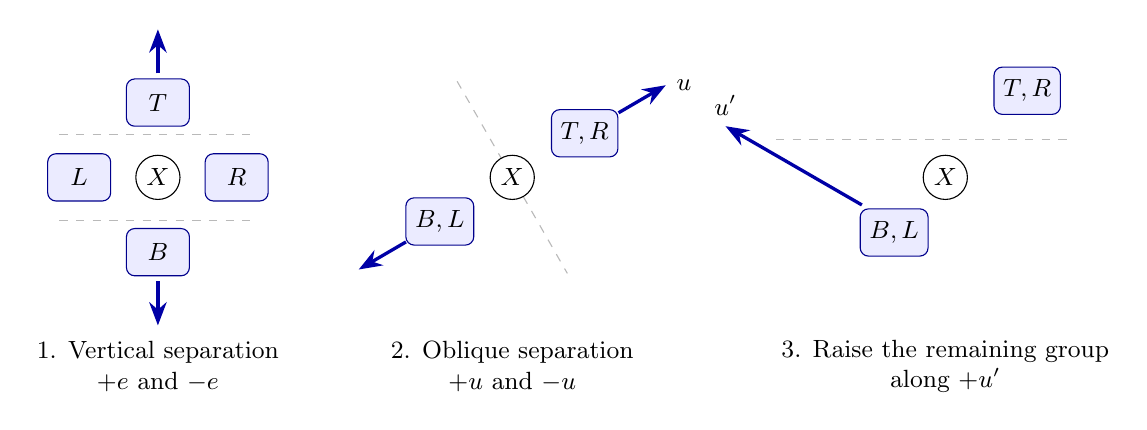
\begin{tikzpicture}[x=1cm,y=1cm,>=Stealth,
  group/.style={draw=blue!55!black,fill=blue!8,rounded corners=3pt,
                minimum width=8mm,minimum height=6mm,font=\small},
  ins/.style={circle,draw=black,fill=white,inner sep=2pt,font=\small},
  move/.style={->,very thick,draw=blue!65!black},
  guide/.style={dashed,gray!55}]
\begin{scope}[shift={(0,0)}]
 \draw[guide] (-1.25,.55)--(1.25,.55);
 \draw[guide] (-1.25,-.55)--(1.25,-.55);
 \node[ins] at (0,0) {$X$};
 \node[group] at (-1,0) {$L$};
 \node[group] at (1,0) {$R$};
 \node[group] at (0,.95) {$T$};
 \node[group] at (0,-.95) {$B$};
 \draw[move] (0,1.32)--(0,1.88);
 \draw[move] (0,-1.32)--(0,-1.88);
 \node[font=\small,align=center] at (0,-2.4)
    {1. Vertical separation\\$+e$ and $-e$};
\end{scope}
\begin{scope}[shift={(4.5,0)}]
 \draw[guide] (-.7,1.22)--(.7,-1.22);
 \node[ins] at (0,0) {$X$};
 \node[group] at (.92,.56) {$T,R$};
 \node[group] at (-.92,-.56) {$B,L$};
 \draw[move] (1.35,.82)--(1.95,1.17)
    node[right,font=\small] {$u$};
 \draw[move] (-1.35,-.82)--(-1.95,-1.17);
 \node[font=\small,align=center] at (0,-2.4)
    {2. Oblique separation\\$+u$ and $-u$};
\end{scope}
\begin{scope}[shift={(10,0)}]
 \node[ins] at (0,0) {$X$};
 \node[group] at (1.04,1.1) {$T,R$};
 \node[group] at (-.65,-.7) {$B,L$};
 \draw[move] (-1.06,-.35)--(-2.792,.65)
    node[above,font=\small] {$u'$};
 \draw[guide] (-2.15,.48)--(1.55,.48);
 \node[font=\small,align=center] at (0,-2.4)
    {3. Raise the remaining group\\along $+u'$};
\end{scope}
\end{tikzpicture}


 \caption{The three normal directions used to move the obstacles.
 Each shaded group denotes all of its arc obstacles and local test
 factors.  The insertion $X$ stays fixed.  Vertical moves first
 separate $T$ and $B$; the $u$ moves separate $T\cup R$ and
 $B\cup L$; for a sufficiently large final displacement, the
 $u'$ move places the latter above $X$.
 The relation $u\cdot u'=-1/2$ supplies the projection gap for
 the last move.  Distances are chosen successively; the drawing is
 schematic.}\label{fig:pin-moving}
\end{figure}

\subsection{Equal offsets and filling the gaps}

Keep $\mathcal W$ fixed.  Around each selected intersection choose
a small physical neighborhood contained in its single-color
window, disjoint from all test disks and from all other such
neighborhoods.  In particular there are no $W$ pins in these
neighborhoods.  Let $r>0$ be a sufficiently small fixed size for
them.  Shrink the gaps so that each lies within a ball of radius
$a\ll r$ about its intersection.  This is possible by
transversality.  Constants in what follows can depend on
$\mathcal W$ and $r$, but not on $a$ or on sufficiently small
$\delta$.  We write $o_\delta(1)$ with $a$ fixed.

Let $\mu_{\delta,a}$ be the plane law conditioned on the gapped
pins.  Let $\mu^{=}_{\delta,a}=\mu_{\delta,a}(\,\cdot\mid E)$,
whenever $E$ has positive probability.  Finally let
$\mu_{\delta,0}$ denote the filled bracket.  All these notations
refer to one chosen sign of the bracket.

\begin{lemma}[Gap filling]\label{lem:gap-filling}
There are $\beta>0$ and a function $\epsilon(a)\to0$ as
$a\downarrow0$ such that
\begin{equation}\label{eq:offset-high-probability}
 \limsup_{\delta\downarrow0}\mu_{\delta,a}(E^c)
        \le\epsilon(a).
\end{equation}
If $\mathscr I_\delta$ is the joint increment information in the
fixed test disks, then
\begin{equation}\label{eq:gap-tv}
 \limsup_{\delta\downarrow0}
 \big\|\mu^{=}_{\delta,a}|_{\mathscr I_\delta}
          -\mu_{\delta,0}|_{\mathscr I_\delta}\big\|_{\rm TV}
       \le\epsilon(a).
\end{equation}
For every finite $p$, and for all sufficiently small $a$, the
variables $X_\delta$ have uniformly bounded $p$th moments under
$\mu^{=}_{\delta,a}$ and under $\mu_{\delta,0}$, in the sense
of a bound on $\limsup_{\delta\downarrow0}$ independent of $a$.
No such uniform assertion is needed for the law conditioned on
$E^c$.
\end{lemma}

\begin{proof}
First replace each requirement $W=+$ by the requirement that $W$
be constant on that subpath, and call the resulting edge equalities
$E_0$.  If there are $M$ prescribed subpaths, then, conditional on
$B$ and $E_0$, requiring all their component labels to be plus
has probability between $2^{-M}$ and one.  The number $M$ is
fixed by the original windows and does not grow as gaps shrink.

Consider one gap.  In the annulus from scale $Ca$ to scale $r$,
the only pins are $B$ pins of the desired window sign.  There are
no $E_0$ edges there.  The favorable-pin version of
\cref{lem:buffer-circuits}, used in a logarithmic collection of
separated annular slots, therefore gives a double circuit of
that sign surrounding the gap except with probability
\[
 C(a/r)^\beta+o_\delta(1).
\]
This estimate holds before any offset equality has been imposed.
The two adjoining pinned boundary arms leave the neighborhood,
so a surrounding dual circuit crosses each of them.  At a crossing
both incident primal sites have the window sign.  Consecutive
edges of a double circuit also share a connected chain of sites
of that sign.  Thus the circuit joins the two pinned arms through
a connected constant-$B$ chain.  The adjacent-pair argument of
\cref{lem:boundary-brackets} forces the same lifted pair on both
arms.  Their offsets are therefore equal.

The gap adjacency graph of the remaining boundary arcs is a
cycle, hence connected.  Circuits around all the gaps force every
$t_i$ to agree.  A union bound over the fixed number of gaps,
followed by restoration of the $W=+$ labels at cost at most
$2^M$, proves \eqref{eq:offset-high-probability}, with for
example a constant multiple of $(a/r)^\beta$ as the error.
In particular $\mu_{\delta,a}(E)$ is bounded away from zero for
small $a$ and then small $\delta$.

For the coupling assertion first work with $E_0$ and fill only
one gap.  All the new $B$ pins have the same sign.  The $B$
marginals before and after adding them are ordered, by
\cref{lem:spin-fkg}.  Use the stopping coupling of \cref{sec:cuts}, based on
\cref{lem:double-cut}, exploring outwards from the gap and
coupling the queried values in this order.  In the more adverse
law a double circuit of the added sign occurs before the search
leaves the window neighborhood with failure probability at most
$C(a/r)^\beta+o_\delta(1)$, by the same favorable-pin estimate.
On success it is a common double circuit in the two laws.  All
changed constraints are on its gap side; no $E_0$ edge crosses it.
The conditional law on its other side is therefore identical.
Sample that side identically, including its $W$ components.

Do this successively at the finitely many gaps.  Searches stay in
disjoint window neighborhoods.  The resulting coupling matches
the joint increments in every test disk and all the $W$ labels
that must subsequently be checked, except with probability
tending to zero with $a$.  This last point uses that the label
sites are outside the single-color window neighborhoods.  If two
laws can be coupled with error $\varepsilon$ on variables
including an event $L$, and both give $L$ probability at least
$c>0$, their restrictions conditioned on $L$ differ in total
variation by at most $2\varepsilon/c$.  Indeed, for any event
$A$ the numerators $\PP(A\cap L)$ differ by at most
$\varepsilon$, as do the two denominators, and division gives
the stated bound.  Applying this with $c=2^{-M}$ restores all
the required plus labels.  It proves the claimed approximation
between the unconditioned-offset gapped law and the filled law.
Conditioning the former additionally on $E$ changes any marginal
by at most $\mu_{\delta,a}(E^c)$.  This proves
\eqref{eq:gap-tv}, after enlarging $\epsilon(a)$.

It remains to check the uniform moments under equal offsets.
Fix an annular buffer around $K_0$, with fixed inner and outer
radii and positive clearance from $K_0$.  Choose its filled
interior compactly contained in $D$ and disjoint from all gap
neighborhoods, so the buffer and its interior contain no pins.
Conditional just on the pins, a
double $B$ cut in this buffer has probability at least a fixed
$c_0>0$.  This follows from the local cut estimate and the
bounded cost of the plus labels.  By
\eqref{eq:offset-high-probability}, its probability under
additional conditioning on $E$ is at least $c_0/2$ for all
sufficiently small $a$ and then small mesh.  Moreover $E$ is
measurable outside this cut: relative heights between the
representatives can be evaluated on paths in the connected
exterior of a disk containing the buffer.  Such paths avoid the
unrevealed interior of the cut.  The usual outside-in cut
exploration therefore leaves a Gibbs interior with its
bounded-range trace, even after $E$ is imposed.

All offsets are now common.  Anchoring one representative makes
the interval restrictions fixed integer intervals, so rounded
midpoints require no parity classes.  Together with the fixed
buffer, these observations verify the hypotheses of
\cref{cor:equal-offset-moments}; it
gives the asserted bounds uniformly as the gaps close.  The
filled law has bounded boundary data by
\cref{lem:boundary-brackets}, and
\cref{prop:smearing-moments} gives its bounds.  This argument
does not estimate the exceptional unequal-offset law.
\end{proof}

\begin{proposition}[Bracket identity]\label{prop:bracket-identity}
Fix a window system $\mathcal W$ for a finite grid
$\mathcal L$, and either bracket from
\cref{lem:boundary-brackets}.  Let $K_0,\ldots,K_q\Subset D$
be disks, with $K_0$ at positive distance from every $K_j$,
$j\ge1$, and let $X_\delta,F_\delta$ be as in
\eqref{eq:pins-insertion}.  Suppose there are two levels
$\ell_-<\ell_+$ in $\mathcal L$ such that:
\begin{enumerate}[label=\textnormal{(\roman*)}]
\item $K_0$ is strictly between the two levels, and both levels
      avoid every spectator disk $K_j$ with positive margin;
\item after opening sufficiently small gaps inside their
      corresponding windows, every pin arc and spectator disk
      in the middle band belongs to one of the two strictly
      separated $u$-projection families in
      \eqref{eq:middle-projections}.
\end{enumerate}
Then
\begin{equation}\label{eq:bracket-identity}
 \lim_{\delta\downarrow0}
   \EE_{\mu^{\pm,\mathcal W}_\delta}
       [H_\delta(\Delta\phi)F_\delta]=0.
\end{equation}
In particular it applies to products of bounded continuous
functions of finitely many smooth zero-total tests in each
$K_j$.  There is no disjointness requirement between spectator
disks.  For this latter class the identity passes to any
subsequential distributional limit of the bracket laws.

For any fixed bound $q$ on the number of spectator disks these
geometric hypotheses can be arranged locally as follows.  Fix
$x\in D$ and $\rho>0$ with $\overline{B(x,\rho)}\subset D$.
Take $K_0$ sufficiently small about $x$, and take at most $q$
spectator disks of sufficiently small radii, all outside
$B(x,\rho)$.  From a sufficiently dense grid of regular levels
one can choose the two levels within a fixed small fraction of
$\rho$ above and below $x$.  The choices and smallness bounds
depend on $q$ and $\rho$, not on the number of terms in a later
linear combination of such products.
\end{proposition}

\begin{proof}
At fixed gaps, \cref{prop:pin-product} gives
$\PP(P)/J_\delta\ge c_a>0$.  By
\cref{lem:gap-filling}, for all sufficiently small fixed $a$,
$\PP(E\mid P)\ge1/2$ at small mesh.  Division of
\eqref{eq:gapped-equal-offset-identity} by
$\PP(P\cap E)/J_\delta$ therefore gives
\begin{equation}\label{eq:conditional-gapped-identity}
 \lim_{\delta\downarrow0}
    \EE_{\mu^{=}_{\delta,a}}[X_\delta F_\delta]=0.
\end{equation}
The positive number $c_a$ may tend to zero as $a\downarrow0$;
it is used only with $a$ fixed.

Let $X^{(T)}=\max(-T,\min(X,T))$ and put
$M=\sup_\delta\|F_\delta\|_\infty$.  The total variation bound
in \cref{lem:gap-filling} applies to $X^{(T)}F_\delta$, which
is a bounded function of the joint test increments.  The same
lemma, at any $p>1$, bounds the truncation errors under the
equal-offset and filled laws by $C_pM T^{1-p}$.  Consequently
\[
 \limsup_{\delta\downarrow0}
 \left|\EE_{\mu_{\delta,0}}[X_\delta F_\delta]\right|
 \le 2MT\epsilon(a)+C_pM T^{1-p}.
\]
First send $a\downarrow0$ and then $T\to\infty$.  This proves
\eqref{eq:bracket-identity}.  For bounded continuous functions
of smooth tests, distributional convergence and the same
uniform integrability pass the expectation to a subsequential
limit.

For completeness, here is a quantitative choice of the local
geometry in the last assertion.  Translate $x$ to the origin.
Take $K_0\subset B(0,\rho/1000)$ and seek levels in
$(\rho/40,\rho/20)$ and $(-\rho/20,-\rho/40)$.
Choose spectator radii so small that the total length of their
vertical projections is less than half the length of either
candidate interval; a bound $\rho/(1000(q+1))$ on each radius
suffices.  There is then a nonempty open subinterval of each
candidate interval avoiding all spectator disks.  Regular values
are dense, so a sufficiently dense regular grid supplies both
levels, with positive margins.

Every boundary point in the resulting middle band is outside
$B(0,\rho)$.  The same is true of every middle spectator disk
by assumption.  Since $|y|<\rho/20$ there, each such point has
$|x|>\sqrt{1-1/400}\,\rho$.  Its $u$-projection
$(\sqrt3/2)x+y/2$ consequently has magnitude greater than
$\rho/2$, with the sign of $x$.  A connected middle arc or
disk cannot change that sign.  Thus
\eqref{eq:middle-projections} holds with ample margin, whereas
all projections of $K_0$ have magnitude at most $\rho/1000$.
Small gaps and lattice approximation errors preserve the
strict inequalities.  This proves the geometric assertion.
\end{proof}

The order of limits is now explicit.  The identity for a fixed
filled window system is proved by first sending the mesh to
zero at fixed positive gaps and then shrinking those gaps.
In the boundary comparison below, one subsequently shrinks
the windows for each fixed finite grid, and only then refines
the grid.  The bracket order alone does not identify its law
with the true boundary law; the next section supplies the
boundary information needed for that step.

\section{A height arch at a constant boundary arc}\label{sec:boundary}

We now recover the boundary information lost in the single-color windows.
Near an arc with prescribed height $k$, we construct a path of height at
least $k$ that joins the boundary on both sides of a small exceptional
piece.  Closing this path through the exterior separates that piece from
the rest of the domain.  The estimate uses the actual conditional Gibbs
law and will also apply to the new boundary traces exposed during this
separation.  In \cref{sec:limits}, lower and upper versions identify both
the boundary mean and its mixed moments with distant observations.

\paragraph{Regions, fixed sites, and artificial exterior.}
All graphs in this section are embedded in the triangular lattice of mesh
$\delta$.  A \emph{skeleton} is a finite connected union of lattice edges.
The free sites of a region lie in bounded faces of its skeleton.  Every
neighbor of a free site is either free or a fixed skeleton site; the latter
sites are its \emph{usable boundary}.  Conditional on the values $\eta$ at
the usable boundary, the height is uniform among the admissible integer
Lipschitz extensions.  We always assume that this set is nonempty.
Only usable boundary values enter this specification.

Initially the skeleton $S_0$ is a polygon boundary.  We also allow it to be
the union of that boundary and finitely many simple lattice circuits meeting
it.  The additional circuits cut off small boundary patches; the chosen
remaining free regions are on the other side.  Vertices in the removed
patches, and vertices exterior to the original polygon, will be declared
open artificially.  Usable boundary sites are never declared open
artificially.  Thus, at threshold $a$, the open sites are
\begin{equation}\label{eq:boundary-open-sites}
 \{v\text{ free or usable}:H(v)\ge a\}
 \ \cup\ \{v\text{ outside the region and its usable boundary}\}.
\end{equation}
When an additional separator is exposed, its usable sites carry their
actual exposed heights.  In particular, this convention does not discard a
new boundary condition.

Write $Q_r=p+[-r,r]^2$ in tangent and inward-normal coordinates at a smooth
boundary point $p$.  The interior is on the positive normal side.
An open site circuit surrounding $Q_r$ is called an \emph{arch separator}:
its part in the domain joins the clean boundary on the two sides, and its
remaining part can run through the artificial exterior.  It separates the
free sites near $p$ from remote boundary data.

\begin{theorem}[Constant-arc arch estimate]\label{thm:boundary-arches}
There are constants $M>1$, $c,C>0$, and a positive geometric tolerance with
the following property.  Fix a positive integer $N$ and scales
\begin{equation}\label{eq:arch-scales}
  16r<\ell_1<\cdots<\ell_N<R/10,
  \qquad \ell_{i+1}\ge M\ell_i.
\end{equation}
Suppose that, in $Q_R$, the limiting boundary is the single graph
$y=f(x)$, with $f(0)=f'(0)=0$ and $\|f'\|_\infty$ smaller than the
geometric tolerance, and that its inward side is above this graph.  The
original polygon boundary is a sufficiently fine uniform parametric
approximation of this arc and has the same inside and outside away from
its shrinking boundary neighborhood.  Its approximation error, divided by
$\ell_1$, tends to zero.  A smooth boundary has these properties after
decreasing the fixed outer scale.
Allow, in addition, a fixed finite number of boundary-attached patch
replacements as above, whose diameters are sufficiently small relative to
the selected scales.  Suppose that the actual usable boundary data satisfy
\begin{equation}\label{eq:arch-boundary-data}
 \eta\ge k-2\quad\hbox{everywhere},
 \qquad
 \eta\ge k\quad\hbox{on the usable boundary in }Q_R\setminus Q_r,
\end{equation}
where $k\in\Z$.  For sufficiently small mesh and sufficiently fine boundary
and replacement approximations,
\begin{equation}\label{eq:arch-high-probability}
 \PP_\eta\bigl(\text{an arch at threshold }k\text{ surrounds }Q_r
       \text{ in }Q_R\bigr)\ge 1-Ce^{-cN}.
\end{equation}
The constants do not depend on the boundary heights or on the number of
vertices in a boundary or separator.  They also do not depend on the fixed
number of tiny replacements; the required approximation accuracy may do so.
There is a reversed statement with $\eta\le k+2$, clean data $\eta\le k$,
and a separator at height at most $k$.
\end{theorem}

The order of quantifiers is part of the statement.  One first chooses the
number and the positive scales of the comparison boxes.  The mesh and the
parametric boundary error then tend to zero, and the diameters of the fixed
finite family of replacements tend to zero relative to these boxes.
Consequently, the error tends to zero as the number of available scales
between a central exception and the end of a clean arc tends to infinity.
There is no assertion uniform over unresolved geometry at the mesh scale.
The lower estimate has no upper bound on $\eta$ as a hypothesis.  It
therefore applies to bounded boundary data and also, conditionally, to the
possibly larger random values revealed on a preliminary separator.

The proof first constructs many pairs of weaker separators, at height
$k-1$.  Selecting the inner separator from its inner side and the outer
separator from its outer side leaves an unexamined Gibbs region between
them.  These retained middle regions are conditionally independent.  In
each one we then build two attachments from the clean boundary at the
required height $k$, and join them by bulk paths.  A fixed positive chance
of this upgrade in each retained region gives the exponential error in
\eqref{eq:arch-high-probability}.

The attachment is the main step: a synthetic mean comparison first detects
the high side of a boundary-entering level contour; two low lateral
barriers then force the adjacent path at height $k$ to rise into the domain.
Closed high islands alone would not give an attachment.  All boxes in this construction
have fixed positive relative margins.  After they have been chosen, the
mesh is small enough that rounding preserves their separation and
intersection properties.

\subsection{An anchored two-interval comparison}

For any $k$, one of the two Gray-code colors, denoted by $t$, and one of its
signs $s$, describe the two adjacent residues in $[k-1,k]$.  The opposite
sign of the same color describes $[k-3,k-2]$.  Denote the complementary
color by $v$.  The transition from the low interval to the high interval
can only be the step
\begin{equation}\label{eq:anchored-transition}
                  k-2\longleftrightarrow k-1.
\end{equation}
The complementary color has the same value, say $c_k$, at both ends of
this step, and this is the same value at every such transition.

Here is the comparison we shall repeatedly use.  On a connected skeleton
$S$, assign the sign $s$ to selected connected portions and $-s$ elsewhere.
Require $v=c_k$ at each of a bounded number $b$ of transition edges, and
anchor the lift by \eqref{eq:anchored-transition} at one of them.  A
constant-$t$ chain stays in one adjacent pair of integers: a nearest-neighbor
step cannot move to the next pair with the same residue color.  A transition
with the prescribed complementary color fixes the next pair.  Connectedness
therefore gives the exact bounds
\begin{equation}\label{eq:synthetic-intervals}
 K\in[k-1,k]\text{ on the high portions},\qquad
 K\in[k-3,k-2]\text{ on the low portions}.
\end{equation}
Extra lattice edges between pinned vertices only impose additional
compatibility; they do not introduce new branches of the lift.  In
particular the prescription is nonempty: taking $v\equiv c_k$ gives just
the two values in \eqref{eq:anchored-transition}.

Construct this synthetic height in a larger, finite, simply connected free
lattice volume containing $S$ and all comparison boxes.  Given $t$, the
complementary color is constant on each component of $t$-changing edges and
its component labels are independent fair signs.  The transition
requirements have conditional probability at least $2^{-b}$.  The same
lower bound holds if some transition sites belong to one component, since
all requested labels are $c_k$.

Suppose the actual boundary is at least $k$ on the selected high portions
and at least $k-2$ elsewhere.  Every possible synthetic usable trace is then
bounded above by the actual trace.  Conditional on its trace, the synthetic
interior is a uniform height Gibbs law.  Height comparison, which follows
from the min/max lattice condition, gives
\begin{equation}\label{eq:synthetic-height-domination}
       K|_{\text{free sites}}\preceq H|_{\text{free sites}}.
\end{equation}
This compares the interiors with their actual fixed traces; no observation
of an unconditioned boundary is substituted for boundary pinning.

The prescriptions used below have at most four transitions on the base
polygon.  For tiny replacements, choose those transition points away from
the attachment neighborhoods and give an entire replacement the local
prescription of its base arc.  Its branch is then anchored through that arc
and it adds no transition.  To justify this uniformly, fix the finitely many
selected boxes and the finitely many replacements first.  Uniform
parametric convergence to a simple smooth arc implies that the attachment
points of a replacement of vanishing diameter lie in one vanishing
parameter interval.  The transition points can be chosen in their prescribed
positive-width buffers outside all these intervals.  No bound on the length
or the number of vertices of a replacement is needed.

\subsection{Preliminary separators and genuine stopping explorations}

\begin{lemma}[Many preliminary pairs]\label{lem:preliminary-circuits}
Under the hypotheses of \cref{thm:boundary-arches}, with probability at least
$1-C_0e^{-c_0N}$, at least $c_0N$ of the selected scales have both an open
site circuit at threshold $k-1$ in
\begin{equation}\label{eq:preliminary-strips}
 Q_{\ell_i}\setminus Q_{\ell_i/2}
       \quad\hbox{and one in}\quad
 Q_{7\ell_i}\setminus Q_{5\ell_i},
\end{equation}
each surrounding its inner box.  Artificially open sites are as in
\eqref{eq:boundary-open-sites}.
\end{lemma}

\begin{proof}
Apply the anchored comparison with the high interval on the two clean
portions of the base arc running from just inside the innermost comparison
strip to beyond the outermost strip.  If a central exception is present,
the two portions are separated by a low central portion.  The other
skeleton sites receive the low interval.  The transition buffers are
disjoint from all the strips and their surrounding buffers.  The bounds in
\eqref{eq:arch-boundary-data} give \eqref{eq:synthetic-height-domination}.

Before imposing the complementary transition labels, every pin in a buffer
used for a $t=s$ double circuit is favorable.  By
\cref{lem:buffer-circuits}, there is a constant $a>0$ such that, conditional
on all first-color spins outside a block buffer, a pair of such double
circuits in slightly narrower versions of \eqref{eq:preliminary-strips}
has probability at least $a$.  Choose $M$ so that the block buffers are
disjoint.  Successive revelation of these buffers gives the same lower
bound conditional on the preceding outcomes.  Indeed, for $\lambda>0$ and
the success indicators $I_i$,
\[
 \EE\exp\!\left(-\lambda\sum_{i=1}^N I_i\right)
       \le (1-a+ae^{-\lambda})^N.
\]
It follows that $\sum I_i\ge aN/2$ except with probability $C e^{-cN}$.
Requiring at most four complementary labels multiplies this failure bound
by at most $2^4$.

Each double circuit meets the high part of the skeleton: the original
boundary has a segment from the inner box to the exterior of the outer
box.  The adjacent faces along the double circuit all have the same first
color and, by continuation from that intersection, their lifts lie in the
anchored pair $[k-1,k]$.  The corresponding closed primal walk stays within
a bounded number of lattice spacings of the dual circuit and has winding
number one about the inner box.  It contains a simple surrounding site
circuit.  This produces the preliminary circuits in the synthetic height.
The event that at least a given number of pairs exist is increasing in the
height, so \eqref{eq:synthetic-height-domination} transfers its probability
to the actual law.
\end{proof}

We now select the preliminary pairs by exploring the actual height law.
The synthetic configuration used to bound their abundance plays no part
in this selection.

\begin{lemma}[Extremal-circuit stopping]\label{lem:extremal-stopping}
In a deterministic annular strip, good surrounding simple site circuits
have inner and outer envelopes.  The innermost such circuit can be selected
by revealing the strip from its inner side; the outermost can be selected
from its outer side.  In each case the selection and the revealed values
are measurable with respect to the sites on the circuit and on the tested
side.  No height on the untested side is conditioned by the selection.

In particular, in each successful block of
\cref{lem:preliminary-circuits}, select an innermost circuit $C_i^-$ in the
inner strip and an outermost circuit $C_i^+$ in the outer strip.  Conditional
on these selections and the full configuration outside the intervening free
regions, those regions have independent Gibbs interiors with their
revealed boundary values.
\end{lemma}

\begin{proof}
If two surrounding simple cycles have at least two common vertices, their
union is two-vertex-connected.  After deleting any one vertex, the
remaining part of each cycle is connected and the two parts still share a
vertex.  Its complementary face containing the inner box and its unbounded
face therefore have simple cycle boundaries.  These boundaries are the
inner and outer envelopes.  They use only good vertices of the original
cycles and stay in the same strip.  If there is only one common vertex,
the two cycles cannot cross just once.  Since both enclose the inner box,
their interiors are nested.  Disjoint surrounding cycles are nested as
well.  Iterating the envelope operation in the finite strip gives the
extremal circuit, regarded without an orientation.

For a specified good circuit $C$, whether it is the inner extremal circuit
can be decided from its closed inner side in the strip.  A competing
circuit that improved it while partly leaving that side would have an
inner envelope with $C$ that is itself a better good circuit entirely on
that side.  Thus the absence of a better circuit has no dependence on
unseen heights outside $C$.  The outer statement is identical with the
directions reversed.  Equivalently, these statements specify stopping
sigma-fields: on the event that the selected circuit is $C$, the recorded
heights and the selection event are measurable using the deterministic set
consisting of $C$ and its tested side.  One may reveal that entire set,
including bounded pockets.  Failure to find a circuit requires only the
strip itself.

For the selected pairs, let $V_i$ be the actual free sites between $C_i^-$
and $C_i^+$.  Reveal the unsuccessful strips, the tested sides of successful
strips, the selected circuits, and then every site outside $\bigcup_i V_i$.
Call the resulting sigma-field $\mathcal G$.  On every realization of the
selected sets, the preceding measurability statement says that the event
specifying these sets places no condition on the heights in $\bigcup_i V_i$
beyond their recorded boundary values.  The finite Gibbs specification
therefore applies.  Distinct $V_i$ have no interacting edge after their
separators are fixed, giving conditional independence.  Touches with the
original boundary may divide $V_i$ into several bounded faces; the same
argument applies to their union.
\end{proof}

The selected circuits have height at least $k-1$ on their usable sites.
Every usable boundary value of a retained middle problem is consequently at
least $k-2$.  The full strip
\begin{equation}\label{eq:untouched-middle}
                     Q_{5\ell_i}\setminus Q_{\ell_i}
\end{equation}
between them was not searched.  Its original usable boundary, including any
tiny replacements, still has the clean lower bound $k$.  Moreover, each
selected circuit meets the base polygon boundary, so
$S=S_0\cup C_i^-\cup C_i^+$ is connected.  These facts hold on every
realization of $\mathcal G$ and will be the only boundary information used
to upgrade the block.

\subsection{An attachment from the prescribed boundary}

\begin{lemma}[Boundary attachment]\label{lem:boundary-attachment}
Consider a retained middle problem at scale $\ell$.  Near either of the
locations $(-2\ell,0)$ and $(2\ell,0)$, there are fixed constants
$0<d/W_0\ll1$ and $0<W_0/\ell\ll1$ for which the following holds.
If the local boundary and the tiny replacements are within a sufficiently
small fraction of $d$ of the horizontal boundary line, then with probability
at least $a_0>0$ a path of sites at height at least $k$ enters from the clean
boundary band and reaches depth $d$ inside the box of half-width $W_0$.
Its boundary end is connected through good fixed or artificial sites to
the exterior below, within a slight enlargement of the box.  The bound is
uniform in the exposed boundary values of the middle problem.
\end{lemma}

\begin{proof}
Translate the attachment location to the origin.  Take $W_0$ to be a small
fixed fraction of $\ell$, and later take $d$ to be a smaller fixed fraction
of $W_0$.  The two preliminary circuits are outside this box.  The
unobstructed part above the boundary tolerance belongs to one bounded face
of $S$; in particular, a site $x$ close to $(0,3d)$ is free in that face.

\emph{Synthetic boundary and its mean.}
On $S$, prescribe the high interval $[k-1,k]$ on a base subarc near the
origin, of half-width approximately $W_0/4$, and the low interval
$[k-3,k-2]$ elsewhere.  Choose its endpoints so that the high part covers
horizontal width $W_0/8$, lies within horizontal half-width $W_0/3$, and
avoids all tiny replacement attachments.  A replacement attached within
the high portion receives the high prescription throughout.  There are
only two transition labels.  This construction is feasible for all
sufficiently small replacement diameters and gives the synthetic lower
comparison $K$ in \eqref{eq:synthetic-height-domination}.

Let $A$ be the event that a primal path of heights at least $k$ joins this
high patch to depth $d$ inside the attachment box.  This is an increasing
height event, so it is enough to give it positive probability in the
synthetic law.  We shall first use the mean at $x$ to detect which side of
the boundary-entering contours contains $x$, and then show that the high
side forces $A$.

Between radii of order $d$ and a small fixed fraction of $W_0$, annular
buffers centered on the projected boundary contain only favorable $t=s$
pins.  The annular stack estimate gives, except with probability
\begin{equation}\label{eq:attachment-cut-error}
                      e(d/W_0)\longrightarrow0,
\end{equation}
a double $t=s$ circuit surrounding $x$ and meeting the high patch.  The
same bound, multiplied by a fixed factor, holds after the two complementary
labels are required.  Choose such a cut using only the first color.  Its
inner face chain belongs to the anchored pair $[k-1,k]$, and both transition
labels lie outside it.  No component of $t$-changing edges crosses the
double cut.  Thus the complementary labels in its interior, including its
inner cut layer, are all free.  Flipping these labels preserves their
conditional law.  It reverses every interior height increment and swaps
the two values of the anchored cut pair, hence sends
$K$ to $2k-1-K$ there.  The conditional mean at $x$ is therefore $k-1/2$.

We also need a bound on the mean on failure, uniform in the lattice size.
The component potentials in the proof of \cref{lem:component-switch}
give this bound.  On each component of $t$-changing edges, $dt$ extended
by zero has a potential with two values differing by two.  If $t=B$, the
identity
\[
                 d(K+BW/2)=W\,dB
\]
expresses the height difference from the transition anchor to $x$ as an
endpoint term of absolute value at most one, plus the component labels
times their potential differences.  Each potential difference has absolute
value at most two.  If $t=W$, use $d(K-BW/2)=-B\,dW$ instead.
The unprescribed labels have conditional mean zero, and at most two
components have prescribed labels.  Since the anchor has value $k-2$ or
$k-1$, this proves
\begin{equation}\label{eq:attachment-failure-mean}
       \bigl|\EE[K(x)\mid t,\text{transition labels}]-k\bigr|\le C_1
\end{equation}
for every first-color configuration, with an absolute constant $C_1$.
Combining the symmetry on success with this bound gives
\begin{equation}\label{eq:attachment-synthetic-mean}
                  \EE K(x)=k-\tfrac12+O(e(d/W_0)).
\end{equation}
All these arguments take place in a finite free volume around the
construction, so no infinite-volume height or absolute anchor is required.

\emph{Low lateral barriers.}
Around the boundary locations with horizontal offsets $\pm2W_0/3$, use
annuli with inner radius several times $d$ and outer radius less than
$W_0/8$.  All local first-color pins are now favorable to $t=-s$.  With
failure probability again tending to zero with $d/W_0$, each side contains
a double $t=-s$ circuit meeting the low skeleton.  Its face paths have the
anchored low values and include a path from the low skeleton to above
depth $3d$, inside the horizontal band of width $W_0/4$ about that side
location.  Write $L$ for the event that both such lateral barriers exist.
They have height at most $k-2$ in the synthetic problem.
The estimates survive the same two complementary labels.  We may increase
the lower end of the annular range by a fixed factor when a little more
vertical clearance is needed.

For the planar separation below, continue each barrier along its local low
skeleton arc and then through the exterior to a line below the boundary
band.  Uniform parametric approximation keeps this continuation in a
slightly enlarged lateral strip; a tiny replacement attaches to the same
local base arc.  The skeleton portion is outside the high patch and is
low throughout.  The exterior portion is only a geometric continuation,
which a contour lying in the face cannot cross.  Thus the two barriers
separate the high patch laterally all the way through the boundary band.

\emph{The mean detects a side of the open contours.}
Condition on the synthetic trace on the whole skeleton $S$.  In its
bounded face containing $x$, follow every dual level path at threshold
$k-1/2$ that enters through a skeleton edge.  At each crossed edge, the
adjacent heights are exactly $k-1,k$.  On entering a triangle, those two
values force its third value to be one of $k-1,k$, and hence determine the
next crossed edge.  The exploration only reveals the adjacent values of
the paths being followed.  Exhaust all boundary crossings in this way,
including crossings on either side of a skeleton edge bordering a slit
in the face.

Conditional on these open paths and their lips, their occurrence imposes
only the indicated fixed vertex values.  Any admissible completion with
those values has the same open paths, by the degree-two rule and exhaustion
of the boundary crossings.  Unseen closed contours remain unrestricted.
The remaining free components therefore have their Gibbs laws.

Cut the face along the exposed open paths.  Their lips have known sides:
the $k$ lip is high and the $k-1$ lip is low.  Together with the threshold
signs of the skeleton trace, these sides label every resulting geometric
cell high or low.  Here is why these labels are consistent even when the
skeleton boundary has slits.  A closed threshold contour in this face
cannot enclose a skeleton site, since the connected skeleton continues
outside the contour and cannot cross it.  It cannot enclose part of an
exposed open path either: that path continues to the skeleton and contours
do not intersect.  In the full threshold-sign picture, one may therefore
erase the closed contours, filling each outermost enclosed region with
its exterior sign, without changing any recorded skeleton or lip sign.
The remaining sign is constant in each cell cut out by the open paths.
This proves consistency; it is a deterministic explanation, not an
additional revelation or conditioning of the closed contours.

The free primal Gibbs components left by the exploration lie in these
geometric cells; removing the revealed lip vertices may divide a cell
further.  In a low cell every adjacent fixed value is at most $k-1$.
In a high cell every adjacent fixed value is at most $k$: the high
skeleton values and the high lips are exactly $k$, and all other fixed
values satisfy the same ceiling.  Let $U$ be the event that $x$ belongs
to a high cell, including the case that it lies on a revealed high lip.
A revealed low lip belongs to the low case.

Comparison with a constant ceiling, including the deterministic case when
$x$ lies on a revealed lip, yields
\begin{equation}\label{eq:attachment-cell-mean}
 \EE K(x)\le k-1+\PP(U).
\end{equation}
Together with \eqref{eq:attachment-synthetic-mean}, this gives
$\PP(U)\ge1/2-O(e(d/W_0))$.  A closed high island around $x$ does not
suffice for $U$.  Such islands remain inside their unrestricted Gibbs
cells, and comparison controls the cell's mean rather than each of its
height values.

\emph{The correct boundary lip reaches the box.}
The high lip of every exposed open path is a connected primal chain at
height $k$.  Its endpoints are skeleton sites at height $k$, so they lie
on the designated high patch, including any tiny replacements carrying
that patch's prescription.  No endpoint lies on a preliminary circuit or
on another low part of the skeleton.

We claim that $U\cap L\subseteq A$.  Suppose instead that $L$ occurs but
$A$ does not.  Follow a high lip from either of its endpoints on the high
patch.  It cannot cross a low lateral barrier: these are primal paths of
height at most $k-2$, whereas the lip has height $k$.  It cannot leave
through the exterior side of the face.  To pass above a barrier it would
first have to reach depth $d$, already giving $A$.  Consequently every
exposed open path stays between the two barriers and below depth $d$.
This statement concerns all the open paths, since every one of their high
lips starts on the designated high patch.

The site $x$ is at depth $3d$.  Staying above depth $2d$, it can be
joined to one lateral barrier without crossing any exposed open contour.
Following that barrier down to its low skeleton endpoint also crosses
none: all its sites have height at most $k-2$.  The resulting route puts
$x$ in the cell with the low label inherited from that endpoint.  This
contradicts $U$.  The boundary and the tiny replacements stay in a much
shallower band and do not obstruct the deep portion of this route; the
barrier itself supplies the continuation through that band.  Fixed margins
between depths $d$ and $3d$ absorb lattice rounding.

Since $\PP(L^c)=O(e(d/W_0))$, the inclusion proves
\[
 \PP(A)\ge\PP(U)-\PP(L^c)\ge\tfrac12-O(e(d/W_0)).
\]
The mean calculation was not conditioned on the lateral barriers.
Choose $d/W_0$ once so that this bound is at least, say, $1/4$.
The event $A$ asks only for a superlevel path, even though the synthetic
construction produced an exact-height-$k$ lip.  It is therefore increasing,
and \eqref{eq:synthetic-height-domination} gives the same positive lower
bound for the actual height.

Finally, in the actual comparison every usable skeleton site in the local
box is at least $k$; the other skeleton sites there are artificial.  A tiny
replacement is attached to the local base arc, and that arc, with its
parametric slack at the box margins, is connected through open sites to
the exterior below.  For example a path from below stopped at its first
encounter with the base boundary reaches such an open site.  Thus the
attachment has the exterior continuation claimed in the lemma.
\end{proof}

\subsection{Joining the attachments and amplifying across scales}

\begin{lemma}[Upgrade in a retained middle region]\label{lem:arch-upgrade}
For every successful preliminary block, conditional on $\mathcal G$ from
\cref{lem:extremal-stopping}, the probability of an arch separator at
threshold $k$ in its untouched middle is at least an absolute constant
$a_1>0$.
\end{lemma}

\begin{proof}
Fix the realized middle problem.  Its actual boundary has the lower bounds
recorded after \eqref{eq:untouched-middle}.  The two attachments of
\cref{lem:boundary-attachment} have uniform positive probabilities, and
their events are increasing in the actual height.

We first record a bulk path estimate under this same conditional law.
For a box with a fixed relative annular buffer inside the free middle,
compare from below with constant height $k-2$ on its bounding skeleton.
The latter comparison may be realized by fixing both spins of that height
on $S$.  Connectedness of $S$ fixes a common flat lift on every relevant
bounded face.  Its height contours are closed loops: a contour cannot
cross the flat skeleton or enclose just part of a connected skeleton.
Given the unoriented loops, all their jump signs are independent fair signs.
For use of the first-spin circuit estimates, first enforce constancy of
the second spin along $S$.  This is an $E_0$ constraint outside the bulk
buffers.  Since $S$ is connected, specifying its second-spin value costs
one fair component label and does not change the first-spin marginal.

Apply \cref{lem:buffer-circuits} in a fixed number of thinner concentric
buffers, requesting alternating first-spin signs on five double circuits.
All these buffers are inside the free region.  Successive conditional
estimates give a positive probability, uniform in mesh and exposed actual
heights, for this event in the flat comparison.  Between each successive
pair there is a first-spin wall loop surrounding the inner box.  Hence
there are at least four nested height loops in the allocated annulus.

Retain only the event that there are at least four enclosing unoriented
loops in the allocated annulus, forgetting the first-spin event used to
lower-bound its probability.  This event and the choice of four consecutive
enclosing loops depend only on the full unoriented geometry.  Conditional
on that geometry, the height just outside the first chosen loop is $k-2$
plus a sum of other fair loop signs.  It is therefore symmetric about
$k-2$ and independent of the four chosen signs.  With probability at least
$2^{-5}$ it is at least $k-2$ and all four signs are positive.  The inner
face path of the fourth loop is then at least $k$.  Its closed primal walk
has winding number one and contains a surrounding circuit, with only
bounded mesh displacement.  Thus a fixed bulk annulus has a uniformly
positive probability of a circuit at height at least $k$.  Height order
transfers this to the actual middle law.

These bulk circuits give paths along any fixed polygonal tube with positive
width and clearance.  To see the deterministic gluing, place small annuli
along the tube so that consecutive inner disks overlap and each protrudes
beyond the other annulus's outer disk.  Two surrounding circuits cannot
then be disjoint or nested, so they intersect.  A finite string supplies
the desired connected crossing.  Positive association for heights bounds
the probability of the simultaneous increasing circuit events below by the
product of their positive lower bounds.

Use such a tube to cross each attachment box horizontally near depth
$d/2$, extending a little beyond its sides.  Any rising attachment from
the boundary band to depth $d$ intersects this crossbar.  Join the left
and right crossbars by tubes going upward near horizontal locations
$\pm2\ell$, across at depth $2\ell$, and downward on the right.  Tube
widths are much smaller than $d$, and all their bulk boxes have clearance
from the skeleton.  The whole construction lies between $Q_\ell$ and
$\partial Q_{5\ell}$; see \cref{fig:boundary-arches}.

Apply height positive association in the actual conditional Gibbs problem
to the two attachment events and the finite collection of bulk circuit
events.  This gives a fixed lower bound $a_1>0$ for their intersection.
The exterior continuations of the attachments can be joined below the
boundary, around the bottom of $Q_\ell$, through artificial sites and
good local boundary sites.  The resulting closed open walk follows a
rectangle around $Q_\ell$ and has winding number one, so it contains an
open surrounding simple cycle.  The tubes avoid the preliminary circuits;
in particular, the construction has not declared any of their possibly
sub-$k$ usable values artificial.  Every artificial site used here was
already outside the original region or in a removed boundary patch,
which proves the upgrade.
\end{proof}

\begin{figure}[tb]
 \centering
 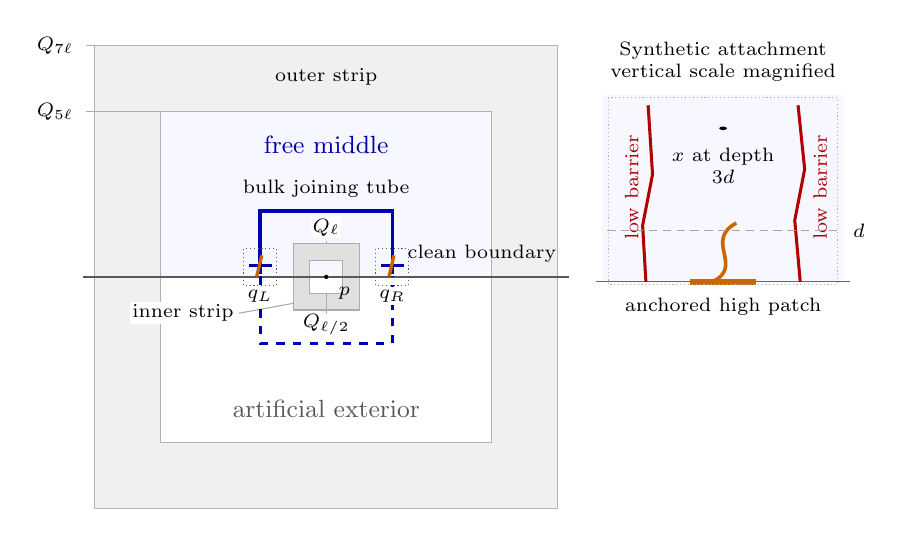
\begin{tikzpicture}[x=0.42cm,y=0.42cm,>=Stealth,font=\small]
  \fill[gray!12,even odd rule] (-7,-7) rectangle (7,7)
                              (-5,-5) rectangle (5,5);
  \fill[gray!24,even odd rule] (-1,-1) rectangle (1,1)
                              (-.5,-.5) rectangle (.5,.5);
  \fill[blue!3] (-5,0) rectangle (5,5);
  \fill[gray!24,even odd rule] (-1,-1) rectangle (1,1)
                              (-.5,-.5) rectangle (.5,.5);
  \draw[gray!60] (-7,-7) rectangle (7,7);
  \draw[gray!60] (-5,-5) rectangle (5,5);
  \draw[gray!65] (-1,-1) rectangle (1,1);
  \draw[gray!65] (-.5,-.5) rectangle (.5,.5);
  \node[anchor=east,font=\scriptsize] at (-7.35,7) {$Q_{7\ell}$};
  \draw[gray!65,thin] (-7.25,7)--(-7,7);
  \node[anchor=east,font=\scriptsize] at (-7.35,5) {$Q_{5\ell}$};
  \draw[gray!65,thin] (-7.25,5)--(-5,5);
  \node[anchor=center,font=\scriptsize,fill=white,inner sep=.5pt] at (0,1.5) {$Q_\ell$};
  \draw[gray!65,thin] (0,1.1)--(0,1);
  \node[anchor=center,font=\scriptsize] at (0,-1.45) {$Q_{\ell/2}$};
  \draw[gray!65,thin] (0,-1.12)--(0,-.5);
  \draw[black!65,thick] (-7.35,0)--(7.35,0);
  \node[anchor=south east,font=\scriptsize] at (7.25,.15) {clean boundary};
  \node[blue!65!black] at (0,4) {free middle};
  \node[gray!70!black] at (0,-4) {artificial exterior};
  \node[font=\scriptsize] at (0,6.05) {outer strip};
  \node[anchor=east,font=\scriptsize,fill=white,inner sep=1pt] at (-2.7,-1.1) {inner strip};
  \draw[gray!65,thin] (-2.65,-1.1)--(-1,-.8);
  \draw[blue!70!black,line width=1.3pt] (-2,.08)--(-2,2)--(2,2)--(2,.08);
  \draw[blue!70!black,line width=1.3pt] (-2.35,.35)--(-1.65,.35);
  \draw[blue!70!black,line width=1.3pt] (1.65,.35)--(2.35,.35);
  \draw[blue!70!black,dashed,line width=1.1pt]
       (-2,.02)--(-2,-2)--(2,-2)--(2,.02);
  \draw[orange!80!black,line width=1.2pt] (-2.1,.02)--(-1.95,.65);
  \draw[orange!80!black,line width=1.2pt] (1.9,.02)--(2.05,.65);
  \draw[black!65,densely dotted] (-2.5,-.25) rectangle (-1.5,.85);
  \draw[black!65,densely dotted] (1.5,-.25) rectangle (2.5,.85);
  \fill (0,0) circle (.065);
  \node[anchor=north west,font=\scriptsize] at (.08,-.02) {$p$};
  \node[anchor=north,font=\scriptsize,fill=white,inner sep=1pt] at (-2,-.3) {$q_L$};
  \node[anchor=north,font=\scriptsize,fill=white,inner sep=1pt] at (2,-.3) {$q_R$};
  \node[anchor=south,font=\scriptsize] at (0,2.12) {bulk joining tube};
  \begin{scope}[shift={(12,-.15)},x=1.4cm,y=0.65cm]
    \fill[blue!3] (-1.1,0) rectangle (1.1,3.65);
    \draw[black!60] (-1.15,0)--(1.15,0);
    \draw[orange!80!black,line width=2pt] (-.3,0)--(.3,0);
    \node[anchor=north,font=\scriptsize] at (0,-.13) {anchored high patch};
    \draw[red!70!black,line width=1.1pt] (-.70,0)--(-.73,1.1)--(-.64,2.1)--(-.68,3.45);
    \draw[red!70!black,line width=1.1pt] (.70,0)--(.65,1.2)--(.74,2.2)--(.68,3.45);
    \node[rotate=90,font=\scriptsize,red!65!black] at (-.83,1.85) {low barrier};
    \node[rotate=90,font=\scriptsize,red!65!black] at (.88,1.85) {low barrier};
    \draw[orange!80!black,line width=1.3pt] (-.1,0).. controls (.2,.3) and (-.18,.8)..(.12,1.15);
    \draw[gray!70,densely dashed] (-1.05,1)--(1.05,1);
    \node[anchor=west,font=\scriptsize] at (1.09,1) {$d$};
    \fill (0,3) circle (.035);
    \node[anchor=north,align=center,font=\scriptsize] at (0,2.8) {$x$ at depth\\$3d$};
    \draw[gray!60,densely dotted] (-1.04,-.05) rectangle (1.04,3.6);
    \node[align=center,font=\scriptsize] at (0,4.3) {Synthetic attachment\\vertical scale magnified};
  \end{scope}
\end{tikzpicture}


 \caption{A retained block in tangent coordinates.  The four labeled squares
 determine the two searched strips; the attachment boxes and path widths are
 enlarged for legibility.  The two shaded strips contain the preliminary separators.
 Their facing sides leave the middle Gibbs region unsearched.  The blue
 route uses two boundary attachments, horizontal crossbars, and bulk
 paths at positive clearance in the actual height law.  The right detail
 shows the synthetic low-barrier argument used to prove an attachment;
 its barriers are not imposed in the actual law.  The dashed lower route
 uses the artificial exterior.  All displayed paths are schematic corridors,
 not a prescribed realization of the random separator.}
 \label{fig:boundary-arches}
\end{figure}

\begin{proof}[Proof of \cref{thm:boundary-arches}]
Let $Z$ be the number of successful preliminary blocks.
\Cref{lem:preliminary-circuits} gives
$\PP(Z<c_0N)\le C_0e^{-c_0N}$.  Use the actual-height stopping sigma-field
$\mathcal G$ of \cref{lem:extremal-stopping}.  Conditional on it, the retained
middle regions have independent Gibbs laws, and
\cref{lem:arch-upgrade} gives success probability at least $a_1$ in each.
Consequently
\[
 \PP(\text{no upgraded block})
 \le C_0e^{-c_0N}+(1-a_1)^{c_0N}
 \le Ce^{-cN}.
\]
Every upgraded circuit surrounds $Q_r$ and lies in $Q_R$ by
\eqref{eq:arch-scales}.  This proves
\eqref{eq:arch-high-probability}.  Applying the argument to $-H$ proves the
reversed assertion.
\end{proof}

\begin{corollary}[Random traces and tiny boundary replacements]
\label{cor:boundary-robustness}
The arch estimate remains valid conditional on an exterior sigma-field
whenever, conditional on that field, the remaining free heights have a
uniform Gibbs law and their actual usable boundary data obey
\eqref{eq:arch-boundary-data}.  It also remains valid after a fixed finite
number of boundary-attached patches have been removed by exposed simple
circuits, provided the same data bounds hold on the new usable boundary.

For a prescribed error, first fix a finite collection of arch scales and
their boxes.  The replacement diameters, boundary approximation errors, and
mesh may then be made sufficiently small for all comparisons.  The success
constants of the resulting blocks have no factor depending on the number
of microscopic pins or on the fixed number of replacements.
\end{corollary}

\begin{proof}
Every probabilistic lower bound in the proof is uniform in the specified
trace; only its displayed one-sided bounds were used.  It may therefore be
applied to each conditional trace.  A boundary-attached replacement keeps
the skeleton connected and preserves the full-neighborhood condition for
the retained free sites.  For fixed scales, sufficiently small replacements
stay in the shallow boundary tolerance and do not meet the bulk tubes.
The transition points of the synthetic prescriptions can be chosen away
from all attachment neighborhoods, as explained after
\eqref{eq:synthetic-height-domination}.  The number of complementary labels
is consequently still at most four in the preliminary construction and at
most two in each attachment construction.  These are the only label costs
in the proof.  The geometric approximation threshold may depend on the
finite family, but none of the block probability constants does.
\end{proof}

\section{Limits, boundary traces, and absolute-height identities}
\label{sec:limits}

We continue to use the integer height $H_\delta=(h_\delta-1)/2$,
and write $H_\delta(f)=\int H_\delta(x)f(x)\,dx$. All tests in this
section are supported in an eventual interior compact of $D$. Thus an
arbitrary extension from $D_\delta$ to $D$, for example extension by zero,
has no effect on the limits under consideration. A bracket means one of
the two filled-window comparison laws of
\cref{prop:bracket-identity}. Its boundary trace, although random, takes
values in $[-2,1]$.

\begin{proposition}[Tightness and convergence of moments]
\label{prop:tightness}
The true fields and all the bracket fields are tight in
$H^{-t}_{\mathrm{loc}}(D)$ for every $t>1$. For $K\Subset D$, $p<\infty$,
and tests supported in $K$,
\begin{equation}
 \sup_\delta\norm{H_\delta(f)}_{L^p}
       \le C_{K,p}\norm{f}_{\infty}.
 \label{eq:local-test-moments}
\end{equation}
The constants are uniform over these bracket laws. Along convergence in
law, every finite joint test moment converges. These assertions hold
also for any fixed finite collection of fields in a coupling.
\end{proposition}

\begin{proof}
Cover $K$ by finitely many balls whose radii are a sufficiently small
fixed fraction of their distance from $\partial D$, and use a partition
of unity. The smearing estimate of \cref{prop:smearing-moments}, applied
to the positive and negative parts on each ball, gives
\eqref{eq:local-test-moments}. For brackets, condition first on the
boundary trace. Its uniform bound gives the same constants before and
after averaging over that trace.

For completeness, place a cutoff $\chi\in C_c^\infty(D)$ in a fixed
square, regarded as a flat torus, and let $e_n$, $n\in\Z^2$, be its
normalized Fourier basis. Since $\norm{\chi e_n}_\infty$ is bounded
independently of $n$, for $s>1$ we have
\begin{equation}
 \sup_\delta\EE\norm{\chi H_\delta}_{H^{-s}}^2
 =\sup_\delta\sum_{n\in\Z^2}(1+|n|^2)^{-s}
                  \EE|H_\delta(\chi\overline{e_n})|^2<\infty.
 \label{eq:sobolev-bound}
\end{equation}
For any $p\ge2$, Minkowski's inequality applied to the sum defining
the squared norm gives its $L^{p/2}$ bound as well, using
\eqref{eq:local-test-moments} at order $p$. If $1<s<t$, the inclusion
$H^{-s}\hookrightarrow H^{-t}$ on this torus is compact: its Fourier
multiplier tends to zero, and truncating the Fourier series gives
finite-rank approximations. Markov's inequality and
\eqref{eq:sobolev-bound} therefore give tightness in $H^{-t}$.
Use a nested countable family of cutoffs equal to one on an exhaustion
of $D$. Choosing the compact-containment probabilities for its members
with a summable error gives tightness in the corresponding local
Sobolev space, and hence in distributions.

If $f_1,\ldots,f_j$ are fixed tests, H\"older's inequality and
\eqref{eq:local-test-moments} at order $j(1+\eta)$ bound
$\prod_i H_\delta(f_i)$ in $L^{1+\eta}$, for any fixed $\eta>0$.
It is uniformly integrable. Convergence in law of the test vector
therefore implies convergence of its product expectation. The same
argument applies to mixed products from a finite coupling. The
moment inequalities themselves pass to every limit by truncation.
\end{proof}

Fix once and for all a nonnegative radial function
$\rho\in C_c^\infty(B(0,1))$ with integral one, and set
\[
 \rho_{x,r}(z)=r^{-2}\rho((z-x)/r),\qquad
 d(x)=\dist(x,\partial D).
\]
Choose a sufficiently small fixed $\kappa>0$. The smearing estimate,
first with mesh tending to zero at fixed $x$, also implies
\begin{equation}
 \sup_{x\in D}\norm{H(\rho_{x,\kappa d(x)})}_{L^p}\le C_p
 \label{eq:depth-moment-bound}
\end{equation}
for any subsequential true or bracket limit. Here and below a harmless
change of the constant covers centers in a fixed compact part of $D$.
In particular this bound is valid when the center approaches a marked
point; it requires only bounded boundary data, not a constant arc.

\subsection{The ordered limits have the correct boundary mean}

We specify the limits of brackets before using their identities.
Choose increasing finite grids $\mathcal G_n$ whose union is dense
among the transverse regular horizontal levels of $\partial D$ and
which miss the two marks. Each such level has finitely many boundary
intersections. For fixed $n$, choose disjoint windows at these
intersections, avoiding the marks, and denote their maximum size by
$\eta$. At each mesh, height comparison gives a coupling
\begin{equation}
                 H_{\delta,n,\eta}^-
                    \le H_\delta\le H_{\delta,n,\eta}^+.
 \label{eq:ordered-brackets}
\end{equation}
For example, couple each ordered pair and disintegrate over the true
field to join the couplings. Affine interpolation preserves the order.

Start with an arbitrary convergent subsequence of the true laws, with
limit denoted by $H$. For each fixed $n,\eta$ take further joint
subsequences in \eqref{eq:ordered-brackets}; then let $\eta$ decrease
to zero at fixed $n$; finally let $n$ increase. Tightness permits all
these extractions. At every stage the true marginal is the originally
chosen law of $H$. The order persists when tested against nonnegative
smooth functions, because that is a closed condition under
distributional convergence. The use of a countable determining family
of nonnegative tests makes the order simultaneous almost surely.
Write the final triple as $(H^-,H,H^+)$.

Identities from \cref{prop:bracket-identity} pass through these limits.
For bounded continuous functions of local increment tests this follows
from convergence in law and the moment bound for the Laplace
insertion. Every admissible finite selection of grid levels belongs
to all sufficiently late grids. Taking the other insertion to be one
shows that the distributional means $m^-$ and $m^+$ of the final
brackets are harmonic locally throughout $D$. Indeed any interior
point admits two regular levels on opposite sides of a sufficiently
small testing disk. Distributional harmonic functions are smooth,
so these means are ordinary harmonic functions. Comparison with
constant-boundary laws, whose means equal the boundary constant by
height reflection, gives
\begin{equation}
                     -2\le m^-\le m^+\le1.
 \label{eq:bounded-bracket-means}
\end{equation}

\begin{proposition}[Boundary trace and mixed boundary moments]
\label{prop:boundary-trace}
Both limiting bracket means are the harmonic extension $m$ of $g$.
Consequently $H^-=H=H^+$ almost surely in the ordered coupling, and
$\EE H=m$.

Let $p$ be on an open boundary arc on which $g=k$, where $k$ is
$0$ or $-1$, and let $x\to p$ from within $D$. For the true limiting
field put $Y_x=H(\rho_{x,\kappa d(x)})$. If $F$ is a product of a fixed
finite number of height averages supported away from a neighborhood
of $p$, then
\begin{equation}
                      \EE[(Y_x-k)F]\longrightarrow0.
 \label{eq:mixed-boundary-trace}
\end{equation}
The same assertion holds when those averages approach finitely many
other, distinct, nonmarked boundary points, with their radii a fixed
small fraction of their depths. In that assertion the points and their
finite number are fixed before the depths tend to zero.
\end{proposition}

\begin{proof}
We first identify the bracket means. Fix a point $p$ on an open arc
of value $k$, a center $x$ near $p$, and its testing ball of radius
$\kappa d(x)$. Choose finitely many final arch scales surrounding
this ball in a small clean neighborhood of the nearest boundary
projection of $x$. Work initially at finite mesh with a fixed grid
and windows sufficiently small for the construction below, and write
$Y_{\delta,x}$ for the chosen bracket's unit average in the ball.
Two searches will isolate the ball from the exceptional window values
and then from the remote boundary data.

For each window choose a clean censor neighborhood on its constant
arc, of value $k_i$. Choose these neighborhoods disjoint, away from
the marks, small relative to the final arch scales, and small enough
to miss the testing ball. Conditional
on the original bracket trace, all its values are at least $k_i-2$,
and those in this censor neighborhood outside its window are at least
$k_i$. Enclose the entire discrete window and its adjacent sites in
the inner comparison box, with a positive margin before sending the
mesh to zero. Theorem~\ref{thm:boundary-arches} supplies an arch at
level $k_i$ surrounding this box. For a fixed grid there are only
finitely many windows; shrinking them relative to their censor
neighborhoods makes the total failure probability as small as desired.

On success choose the innermost arch by exploring from the window
side, as in \cref{lem:extremal-stopping}. Discard the patch between
the window and this arch, and retain the side away from the window.
This retained side contains the testing ball and has not been
examined by the search. Conditional on the revealed patches and
separator traces, its free heights have their Gibbs law. No original
exceptional vertex is adjacent to a retained free site. The new usable
separator sites carry their actual heights, which are at least $k_i$;
the global lower bounds are also preserved. Thus the first searches
replace the windows by small boundary pieces with the required
one-sided data. They do not condition on the preliminary revelations
used only to prove the arch probability estimate.

Apply \cref{cor:boundary-robustness} at the chosen final scales in
the retained domain. The censor patches are small enough for its
replacement hypothesis. In the chosen clean neighborhood every usable
original or replacement boundary site has height at least $k$.
With high probability there is an arch at level $k$ separating the
testing ball from the remote boundary. Choose the outermost such
arch by searching from the remote side. This time the unexamined
region is the side containing the testing ball, between the final
arch and the clean boundary arc. Its usable boundary consists of
sites on the arch and any original or censor pieces it contains,
all at height at least $k$. Height comparison with constant data
therefore gives conditional mean at least $k$ for $Y_{\delta,x}$.

Let $E_\delta$ denote success of both stages, and expose only the
discarded patches, the remote side of the final arch, and their
usable traces. On $E_\delta$ this information determines the event
and leaves the testing region Gibbs. For any $q>1$ the preceding
conditional comparison gives
\begin{equation}
 \EE(Y_{\delta,x}-k)\ge
       -\norm{Y_{\delta,x}-k}_{L^q}
                           \PP(E_\delta^c)^{1-1/q}.
 \label{eq:boundary-mean-error}
\end{equation}
The norm is bounded by the unconditional comparable-depth smearing
estimate, whose limit form is \eqref{eq:depth-moment-bound}. No
moment estimate after conditioning on censor success is needed.

For the upper bound start afresh from the original bracket trace.
Its global values are at most $k_i+2$, and its clean values in the
$i$th censor neighborhood are at most $k_i$. Use decreasing censor
arches and then a decreasing final arch in the same two stopping
directions. The testing region now has usable boundary at most $k$,
giving the matching upper estimate, with the same H\"older bound on
the failure contribution. This separate
construction is necessary because the lower censor arches carry no
upper bound on their revealed heights.

We make explicit the uniformity that permits the grid limit. Given an
error tolerance, first choose finitely many final arch blocks in a
sufficiently straight part of the limiting smooth arc. They are
available for every sufficiently shallow testing center. For each
fixed grid, choose the outer censor sizes so small that the robust
comparison applies in these blocks; the synthetic interval endpoints
in that comparison avoid all the tiny replacements. By
\cref{cor:boundary-robustness}, the final block estimates do not incur
a factor for the number of replacements. Next decrease the window
sizes so that all censor searches succeed with the desired total
error, and before that take the mesh and boundary approximation
errors to zero. The resulting bound on the mean depends on the final
blocks and the error tolerance, and not on the grid. It thus survives
window limits followed by grid refinement. This is exactly the order
of limits used to define $(H^-,H,H^+)$. Nearest projections and the
uniform smooth-arc estimates allow tangential as well as normal
approaches to $p$.

Since each bracket mean is harmonic, radial averaging recovers its
value at $x$. The two bounds just proved show that its boundary trace
is $k$ on the open arc. Together with
\eqref{eq:bounded-bracket-means}, bounded harmonic uniqueness gives
$m^-=m^+=m$. The two marked points do not change this uniqueness:
for a bounded harmonic function with zero trace elsewhere, compare
its absolute value with its supremum times the harmonic measure of
arbitrarily small boundary neighborhoods of the marks. At any fixed
interior point these harmonic measures tend to zero, since a smooth
domain has a Poisson kernel and single points have zero arclength.

The order now identifies the fields, rather than merely their means.
For every nonnegative test $f$,
$H^+(f)-H^-(f)\ge0$ and its expectation is zero. Thus it vanishes
almost surely. Apply this to a countable dense family of nonnegative
tests and use continuity of distributions. The ordered fields agree
as distributions almost surely, proving the first assertion and
transferring the bracket identities to $H$.

For the mixed assertion no censoring is needed in the true law.
Choose deterministic outer arch neighborhoods that do not meet the
supports of the other observations. First suppose $F\ge0$ is
measurable outside those neighborhoods. On the lower good event
$E_-$, choose the outermost lower arch from the exterior. The event,
the selected trace, and $F$ are measurable in the revealed exterior;
the Gibbs property gives
\[
                  \EE[(Y_x-k)F;E_-]\ge0.
\]
The upper search separately gives an event $E_+$ on which the reverse
inequality holds. These two searches need not share a sigma-field.
For $q>1$, their failure contributions satisfy
\begin{equation}
 -\norm{(Y_x-k)F}_{L^q}\PP(E_-^c)^{1-1/q}
 \le \EE[(Y_x-k)F]
 \le \norm{(Y_x-k)F}_{L^q}\PP(E_+^c)^{1-1/q}.
 \label{eq:weighted-arch-bounds}
\end{equation}
All norms here are bounded by H\"older and the smearing estimates.
For signed $F$, apply the bounds to its positive and negative parts;
they are exterior measurable and have the same moment control.
One uses the actual exterior stopping search at this step, without
retaining any of the preliminary revelations used to prove the arch
probability estimate. The result follows first at finite mesh, then
for limit moments by \cref{prop:tightness} and truncation.

When other observations approach different boundary points, fix that
finite set first and take the outer neighborhoods smaller than their
mutual distances. The observations remain exterior measurable as
their depths decrease. Estimate \eqref{eq:depth-moment-bound} bounds
their moments uniformly, so the same proof gives
\eqref{eq:mixed-boundary-trace} in this joint limiting regime.
\end{proof}

\begin{lemma}[Deterministic boundary reference averages]
\label{lem:boundary-references}
Fix a compact subarc of one open constant boundary arc, with value
$k$. There exist finite averages of comparable-depth unit smearings
near that subarc which converge to $k$ in every finite $L^p$ of the
true limiting field. More precisely, choose $N$ distinct points
$p_1,\ldots,p_N$ in the subarc, let $x_i(t)$ approach $p_i$ normally
at depth $t$, and put
\[
 A_{N,t}=\frac1N\sum_{i=1}^N
       H(\rho_{x_i(t),\kappa d(x_i(t))}).
\]
For all sufficiently small $t$ the balls are disjoint, and
\begin{equation}
 \limsup_{t\downarrow0}\EE|A_{N,t}-k|^2\le\frac C N,
 \qquad
 \sup_{N,t}\norm{A_{N,t}-k}_{L^q}\le C_q.
 \label{eq:boundary-average-variance}
\end{equation}
The second supremum is over admissible small depths. Consequently
$\lim_{N\to\infty}\limsup_{t\downarrow0}
\norm{A_{N,t}-k}_{L^p}=0$ for every finite $p$.
\end{lemma}

\begin{proof}
Write $Y_i(t)$ for the $i$th summand. Uniform comparable-depth
moments give $\EE|Y_i(t)-k|^2\le C$. For $i\ne l$, apply
\eqref{eq:mixed-boundary-trace} with exterior factor $Y_l(t)-k$:
\[
       \EE[(Y_i(t)-k)(Y_l(t)-k)]\longrightarrow0.
\]
Expanding the square, taking the depth limit at fixed $N$, and then
using the diagonal bound proves the first estimate in
\eqref{eq:boundary-average-variance}. Minkowski's inequality gives
the second from \eqref{eq:depth-moment-bound}, uniformly in $N$.
For $p\le2$ use the $L^2$ bound; for $p>2$ interpolate $L^2$ with
an $L^q$ bound for any $q>p$. A diagonal choice of finite depths as
$N$ increases gives the claimed reference sequence. In particular,
we have not asserted that one comparable-depth average, or a fixed
finite collection of them, becomes deterministic.
\end{proof}

\subsection{Absolute moments and the absence of diagonal terms}

Define the distributional moment $T_j$ by
\begin{equation}
 \langle T_j,f_1\otimes\cdots\otimes f_j\rangle
       =\EE\prod_{i=1}^j H(f_i),\qquad T_0=1.
 \label{eq:moment-distributions}
\end{equation}
These are well-defined distributions on $D^j$. For example, the
local Sobolev moment bounds in the proof of \cref{prop:tightness}
permit taking the expectation of the tensor power as a distribution;
equivalently, the continuous multilinear form in
\eqref{eq:moment-distributions} has a distributional kernel. Let
\[
 \mathcal C_j=\{(x_1,\ldots,x_j)\in D^j:x_i\ne x_l\text{ for }i\ne l\}
\]
be the configuration space without collisions.

\begin{proposition}[Harmonicity of absolute-height moments]
\label{prop:moment-harmonicity}
On $\mathcal C_j$, $T_j$ is a smooth function and is harmonic in each
variable separately.
\end{proposition}

\begin{proof}
The identity already transferred to the true law says
\begin{equation}
                     \EE[H(\Delta\phi)F]=0
 \label{eq:true-local-increment-identity}
\end{equation}
for bounded products of localized increment functions satisfying the
separation conditions of \cref{prop:bracket-identity}. In particular,
each factor may be a bounded continuous function of $H(q)$, where
$q$ has integral zero and is supported in a small disk. Moment bounds
and truncation extend the identity to products of finitely many such
$H(q)$'s whenever the same geometric conditions hold. The disks may
overlap one another.

Fix distinct points $x_0,x_2,\ldots,x_j$. Take a small closed disk
about $x_0$ with a larger concentric neighborhood compactly contained
in $D$ and disjoint from the spectator points. Choose spectator
neighborhoods and tests $f_i$ therein, and write $c_i=\int f_i$.
All these neighborhoods can be made as small as needed below. We
will approximate each absolute observation $H(f_i)$ by constants
and local zero-total observations supported a fixed positive distance
from the Laplace insertion.

Choose a unit smooth average $\rho_i$ near $x_i$, and a clean boundary
subarc accessible without entering a fixed larger disk about $x_0$.
Such access is always possible. A path in $D$ that meets the excluded
small disk can be detoured through a concentric annulus compactly
contained in $D$; thus removing this disk does not block a route to
the boundary subarc. For finitely many reference endpoints in
\cref{lem:boundary-references}, join $\rho_i$ to each endpoint by a
finite chain of unit smooth averages
\[
 \rho_{i,n,0}=\rho_i,\ \rho_{i,n,1},\ldots,
 \rho_{i,n,L_{i,n}}=\rho_{x_n(t),\kappa d(x_n(t))}.
\]
Consecutive supports lie in one disk of arbitrarily small prescribed
maximum diameter. Construct this by a sufficiently fine subdivision
of a path in its open tube, reducing the radii as necessary near the
boundary. All chain disks avoid the fixed neighborhood of $x_0$;
different chains need not avoid one another. There is the exact
identity
\begin{align}
 H(f_i)={}&c_i k+H(f_i-c_i\rho_i)
   +\frac{c_i}{N}\sum_{n=1}^N\sum_{l=0}^{L_{i,n}-1}
                 H(\rho_{i,n,l}-\rho_{i,n,l+1})
   +c_i(A_{N,t}-k).
 \label{eq:transport-identity}
\end{align}
Every nonconstant term before the last has total integral zero and
is supported in one small disk. The final term tends to zero in
every required $L^p$, with depth first and then $N$ increasing.

We check the separation geometry uniformly in the number of chain
links. Translate coordinates so that $x_0=0$, and suppose all chain
disks are outside $B(0,R)$. Choose $\ell\ll R$, and support $\phi$
in $B(0,\ell/10)$. Available lower and upper levels lie in
$(-2\ell,-\ell)$ and $(\ell,2\ell)$, respectively. Cap the diameter
of every chain disk, and of each initial spectator neighborhood,
by $\ell/(100j)$. Expand a product of the approximations on the
right side of \eqref{eq:transport-identity}, omitting the last error
term. Each expanded term contains at most $j-1$ disks: it selects
at most one local observation from each original spectator factor.
Thus the total length of the forbidden vertical projections is
less than $\ell/100$ in either available level interval, regardless
of the number or length of the routes. Choose regular levels from
the dense union of grids outside these projections and with positive
clearance.

Any selected disk in the resulting middle band is outside $B(0,R)$
and has vertical coordinate of size at most $2\ell$. It consequently
lies well to the left or right of the insertion, also in projection
along $u=(\sqrt3/2,1/2)$, because $\ell\ll R$. The boundary pieces
in the middle band have the same property by the interior clearance
of $x_0$. These are exactly the geometric conditions of
\cref{prop:bracket-identity}. Each finite expanded term therefore
satisfies \eqref{eq:true-local-increment-identity}; the levels can
depend on that term. There is no requirement that a single pair
avoid every disk in all the routes at once.

For each finite approximation the expanded sum is finite, so its
expectation against $H(\Delta\phi)$ is zero. The approximated
spectator variable differs from $H(f_i)$ by $c_i(A_{N,t}-k)$; in
particular its higher moments stay bounded independently of the
number of links. H\"older's inequality now passes to the $L^p$
reference limit in the unexpanded product. We obtain
\[
             \EE\bigl[H(\Delta\phi)\prod_{i=2}^jH(f_i)\bigr]=0.
\]
This proves distributional harmonicity in the distinguished variable
on a neighborhood of every collision-free configuration. Product
tests suffice by density in the smooth tests on a product
neighborhood. Repeating with each distinguished variable gives
$\Delta_{x_i}T_j=0$ on $\mathcal C_j$. Their sum is the ordinary
elliptic Laplacian on $\R^{2j}$, so distributional harmonic
regularity gives a smooth representative there. The separate
identities then hold classically.
\end{proof}

\begin{lemma}[No distributions supported on collision diagonals]
\label{lem:no-contact}
The smooth function $T_j$ on $\mathcal C_j$ is locally integrable on
$D^j$ and represents its full moment distribution. For $j\ge2$,
$K\Subset D$, and distinct $x_1,\ldots,x_j\in K$, with
$d_* =\min_{i<l}|x_i-x_l|$, it satisfies
\begin{equation}
 |T_j(x_1,\ldots,x_j)|
       \le C_{K,j}\bigl(1+\log_+(1/d_*)\bigr)^{j/2}.
 \label{eq:offdiagonal-log-bound}
\end{equation}
With distinct spectators $y_2,\ldots,y_j$ fixed in the interior,
$T_j(x,y_2,\ldots,y_j)$ is bounded as $x$ approaches any part of
$\partial D$, including the marked points. At a nonmarked point of
an arc of value $k$ its trace is
\begin{equation}
 \lim_{x\to p}T_j(x,y_2,\ldots,y_j)
                  =k\,T_{j-1}(y_2,\ldots,y_j).
 \label{eq:moment-boundary-trace}
\end{equation}
\end{lemma}

\begin{proof}
Radially mollify every variable at the common radius $r$ and denote
the result by $T_j^{(r)}$. For centers in $K$ and sufficiently small
$r$, the smearing bounds and H\"older give
\begin{equation}
 |T_j^{(r)}(x_1,\ldots,x_j)|
  =\left|\EE\prod_{i=1}^j H(\rho_{x_i,r})\right|
       \le C_{K,j}(1+|\log r|)^{j/2},
 \label{eq:common-mollifier-bound}
\end{equation}
even if some centers coincide. When $d_*>2r$, the averaging balls
are disjoint and separate harmonicity gives
$T_j^{(r)}=T_j$ exactly by successive applications of the mean-value
property. Taking $r$ to be a fixed small fraction of $d_*$, with a
fixed upper cutoff depending on $K$, proves
\eqref{eq:offdiagonal-log-bound}. Its right side is integrable on
$K^j$: it is bounded by a constant times one plus the sum over
pairs of powers of $|\log|x_i-x_l||$, and such powers are
integrable in two dimensions.

The collision neighborhood $\{d_*\le2r\}\cap K^j$ has volume
$O_{K,j}(r^2)$. By \eqref{eq:common-mollifier-bound}, the integral
of $|T_j^{(r)}|$ over that neighborhood tends to zero. The integral
there of the off-diagonal function tends to zero by its local
integrability. Off that neighborhood the two functions agree.
Thus $T_j^{(r)}$ converges in $L^1$ on compact sets to the extended
off-diagonal function. It also converges distributionally to the
original $T_j$, by the approximate-identity property. The two are
therefore the same distribution; no additional term supported on
a diagonal remains.

For the boundary claims, choose fixed, disjoint, small radial unit
averages $\rho_i$ at the spectator points. For $x$ sufficiently
near the boundary, its comparable-depth averaging ball is disjoint
from all of them. Separate mean value gives
\[
 T_j(x,y_2,\ldots,y_j)
   =\EE\left[H(\rho_{x,\kappa d(x)})
                         \prod_{i=2}^jH(\rho_i)\right].
\]
H\"older and \eqref{eq:depth-moment-bound} bound this uniformly in
$x$, including approaches to the marks. At a clean point,
\eqref{eq:mixed-boundary-trace} gives its limit as
$k\EE\prod_{i=2}^jH(\rho_i)$, which equals the right side of
\eqref{eq:moment-boundary-trace} by mean value once more.
\end{proof}

\section{Collision coefficients and Gaussian identification}
\label{sec:gaussian}

The preceding section applies to every subsequential true-field law.
Fix one such limit $H$ and its uncentered moment functions $T_j$.
The plane covariance coefficient is
$v=(2\pi)^2c_*>0$, as in \cref{thm:plane-covariance}. We now show
that it determines all moments in $D$.

A related way to identify Gaussian pairings, by cancelling collision
singularities, appears in Kenyon's dimer-height proof
\cite[Lemma~3.1 and Proposition~3.2]{Kenyon2001}.  The singularities there
are computed from explicit determinant formulas.  Duminil-Copin,
Kozlowski, Lammers, and Manolescu use harmonicity and collision asymptotics
to identify higher full-plane increment correlations from the GFF
two-point function
\cite[Section~7.2]{DCKLM2026}.  Here separate harmonicity determines the
form of each singularity, while a stopped local coupling to the plane law
determines its coefficient.  The boundary traces proved in
\cref{sec:limits} then supply harmonic uniqueness in the bounded domain.

\begin{lemma}[The only isolated singularity is logarithmic]
\label{lem:log-singularity}
Fix a collision-free list $(y,\mathbf z)$ of interior points. In a
neighborhood of $x=y$ containing none of the points of $\mathbf z$,
\begin{equation}
 T_j(x,y,\mathbf z)
     =L(y,\mathbf z)\log\frac1{|x-y|}+R(x;y,\mathbf z),
 \label{eq:log-expansion}
\end{equation}
where $R$ extends harmonically across $x=y$ in the first variable.
The function $L$ is smooth on the parameter configuration space.
On compact subsets of that space one can choose a uniform radius
on which $R$, and each fixed order of its first-variable derivatives
on a smaller disk, are uniformly bounded.
\end{lemma}

\begin{proof}
By \cref{prop:moment-harmonicity,lem:no-contact}, the function of $x$
is harmonic on a punctured disk and has at most polylogarithmic
growth at its puncture. The polar Fourier expansion of a harmonic
function there has constant angular part $a+b\log r$ and, in angular
mode $n\ge1$, radial factors $r^n$ and $r^{-n}$. A coefficient of
$r^{-n}$ would grow faster than every power of $\log(1/r)$, so it
vanishes. The remaining positive modes extend harmonically to the
center. This proves \eqref{eq:log-expansion}. This argument can
also be obtained by taking Fourier coefficients on each concentric
circle and solving their radial differential equations; the growth
bound kills the negative coefficients one at a time.

There is a useful parameter formula that supplies the needed
uniformity. Choose a fixed radius $a>0$, small enough for all
$(y,\mathbf z)$ in a parameter neighborhood. Outward differentiation
in the first variable gives
\begin{equation}
 L(y,\mathbf z)
   =-\frac1{2\pi}\int_{|w-y|=a}
                      \partial_{n_w}T_j(w,y,\mathbf z)\,ds_w.
 \label{eq:circle-log-coefficient}
\end{equation}
The integral of the derivative of the removable remainder is zero,
and that of $\log(1/|w-y|)$ is $-2\pi$. Parametrize the circle by
$w=y+a e^{i\theta}$. The integrand is smooth in all parameters on
this fixed collision-free compact set, so $L$ is smooth. Subtract
the logarithmic term from the boundary values on this circle and
use the Poisson formula on its disk. It gives the extension $R$
and bounds all its first-variable derivatives on every fixed
smaller concentric disk, uniformly over compact parameter sets.
This proves in particular the continuity of $L$ needed below,
without inferring it from a nonuniform singular limit.
\end{proof}

\begin{proposition}[Identification of the collision coefficient]
\label{prop:collision-coefficient}
For $j\ge2$ and distinct $(y,\mathbf z)$,
\begin{equation}
                  L(y,\mathbf z)=\frac{v}{2\pi}T_{j-2}(\mathbf z).
 \label{eq:collision-coefficient}
\end{equation}
The convention is $T_0=1$; no centering is made in this identity.
\end{proposition}

\begin{proof}
\emph{A stopped comparison with the plane.}
We first establish precisely the mixing statement used to examine
the collision. Fix an interior center $y_0$, and fixed small
spectator balls away from it. For two smooth zero-integral tests
$\alpha,\beta$ in disjoint bounded disks, put
\[
 \alpha_r(x)=r^{-2}\alpha((x-y_0)/r),\qquad
 \beta_r(x)=r^{-2}\beta((x-y_0)/r).
\]
Their supports lie in $B(y_0,Cr)$. If $F_\delta$ is a product of
height averages on the spectator balls, then, with a plane copy
denoted by $H_\delta^{\mathrm{pl}}$,
\begin{align}
 &\limsup_{\delta\downarrow0}
 \left|\EE[H_\delta(\alpha_r)H_\delta(\beta_r)F_\delta]
    -\EE[H_\delta^{\mathrm{pl}}(\alpha_r)
                 H_\delta^{\mathrm{pl}}(\beta_r)]\,\EE F_\delta\right|
       \longrightarrow0\qquad(r\downarrow0).
 \label{eq:local-product-mixing}
\end{align}
The mesh limit is taken first at every fixed $r$.

Here is the coupling argument, including the absolute exterior
heights. Choose a fixed disk $B(y_0,R_0)\Subset D$ disjoint from
the spectators. In the spin representation of the true problem,
$W$ is fixed on the one connected boundary path. Imposing constancy
there and then its plus label leaves the $B$ marginal unchanged.
The double-cut stack estimate used in \cref{prop:plane-mixing}
therefore applies in this pin-free interior disk. Search from the
outside inward for a double $B$ circuit between radii of order
$r^{1/2}$ and $R_0$. It fails with probability at most a positive
power of $r$. On success the chosen circuit surrounds a disk of
radius comparable to $r^{1/2}$, and the stopping exploration has
not examined its interior.

The absolute heights at all spectator sites can be read in this
exterior. Choose the anchor on the prescribed boundary, with its
known height, and join it to the spectator balls by paths avoiding
$B(y_0,R_0)$. Such paths exist after reducing $R_0$ if needed:
paths in $D$ can be detoured around this interior disk. A finite
family of positive-width tubes and the spectator balls supplies
the same paths in sufficiently fine lattice approximations. The
edge increment formula, summed from the fixed anchor, gives every
height occurring in $F_\delta$ using only exterior spins. Affine
interpolation uses only the adjacent exterior sites. Thus revealing
these observations adds no interior information.

Conditional on the stopping circuit and all exterior spins,
including $W$, its interior is the free-$W$ double-cut law. Indeed
both $B$ values across every cut edge agree, so there is no constraint
on $W$ across it; the stopping rule has imposed no further interior
condition. The common worst-boundary coupling in the proof of
\cref{prop:plane-mixing}, applied inside this circuit, now matches
the spins in $B(y_0,Cr)$ to those of a plane copy with failure
probability at most a positive power of $r/r^{1/2}$. Its bound is
uniform over the exposed exterior. The conditional coupling can
be chosen with the plane law as its second marginal for every
exterior value. That marginal is consequently independent of the
exterior observations. On failure of the first search, choose
the plane copy independently as well. Altogether the matching
failure probability is at most $C r^\gamma$ for some $\gamma>0$,
in the limiting mesh regime.

On the matching event the two zero-total height smearings agree
with their plane versions. Equality of the local increments
determines heights only up to one additive constant, and the zero
integrals remove exactly that constant. The interpolation weights
have the same zero sum. All comparison statements can first be
implemented in finite free spin volumes and then passed to the
plane law.

Finally this coupling controls unbounded products. The true local
smearings have $L^q$ norms at most
$C_q(1+|\log r|)^{1/2}$ by \cref{prop:smearing-moments}; the plane
zero-total smearings have uniformly bounded $L^q$ norms by
\cref{prop:plane-moments}. The fixed spectator product has bounded
moments of every finite order. Applying H\"older with exponent
four to the two insertions, the spectator product, and the failure
indicator bounds the expectation of the product discrepancy by
\begin{equation}
                    C r^{\gamma/4}(1+|\log r|)=o(1).
 \label{eq:mixing-error-log}
\end{equation}
For the plane term the same bound holds with no logarithmic loss.
This proves \eqref{eq:local-product-mixing}. In particular we have
not used an arbitrary conditional spin law after revealing absolute
heights: those heights were first made measurable in the exterior
of an actual stopping cut.

\emph{Extracting the logarithmic coefficient.}
Choose $\alpha,\beta$ so that
\begin{equation}
 J=\iint\alpha(u)\beta(w)\log\frac1{|u-w|}\,du\,dw\ne0.
 \label{eq:nonzero-log-pairing}
\end{equation}
Such tests exist even in disjoint disks. For example, take the
first-coordinate derivatives of radial unit bumps about two points
on a horizontal line, with sufficiently small disjoint supports.
Integration by parts reduces their pairing to the corresponding
mixed derivative of the log kernel averaged over the two bumps.
That derivative is nonzero at their centers and keeps its sign
when the supports are small. Each derivative test has integral
zero.

Use fixed disjoint radial unit mollifiers at the points of
$\mathbf z$, and let $F$ be the product of the resulting height
averages; when $j=2$, take $F=1$. Separate harmonicity gives
$\EE F=T_{j-2}(\mathbf z)$. By \cref{thm:plane-covariance}, the
mesh limit of the plane pairing in
\eqref{eq:local-product-mixing} equals $vJ/(2\pi)$. The log
constant introduced by the rescaling vanishes since both tests
have integral zero. Taking the mesh limit and then $r\downarrow0$
in \eqref{eq:local-product-mixing} therefore yields
\begin{equation}
 \lim_{r\downarrow0}\EE[H(\alpha_r)H(\beta_r)F]
                  =\frac{vJ}{2\pi}T_{j-2}(\mathbf z).
 \label{eq:mixing-coefficient-limit}
\end{equation}

We compute the same limit from \cref{lem:log-singularity}. The two
shrinking supports are disjoint and avoid the spectators. Averaging
the spectator variables radially thus evaluates the moment function
at $\mathbf z$ exactly. The expression on the left of
\eqref{eq:mixing-coefficient-limit} is
\begin{align*}
 \iint\alpha(u)\beta(w)\bigg[
 &L(y_0+rw,\mathbf z)
       \left(\log\frac1r+\log\frac1{|u-w|}\right)\\
 &\hspace{17mm}+R(y_0+ru;y_0+rw,\mathbf z)\bigg]\,du\,dw.
\end{align*}
The term containing $\log(1/r)$ is exactly zero: for each fixed
$w$ its coefficient is independent of $u$, and $\int\alpha=0$.
This cancellation occurs before estimating the variation of $L$;
no modulus of continuity multiplied by $\log(1/r)$ is required.
Continuity of $L$ and the disjoint supports give convergence of
the remaining logarithmic term to $L(y_0,\mathbf z)J$.
For the remainder, subtract
$R(y_0;y_0+rw,\mathbf z)$ inside the $u$ integral. The subtracted
quantity again integrates to zero, and the uniform first-variable
derivative bound in \cref{lem:log-singularity} makes the remaining
integral $O(r)$. The limit is therefore $L(y_0,\mathbf z)J$.
Comparison with \eqref{eq:mixing-coefficient-limit} and $J\ne0$
proves \eqref{eq:collision-coefficient}.
\end{proof}

\begin{theorem}[Gaussian moment recursion]
\label{thm:gaussian-moments}
For distinct points $(x,y_1,\ldots,y_{j-1})$,
\begin{equation}
 T_j(x,\mathbf y)
   =m(x)T_{j-1}(\mathbf y)
      +v\sum_{i=1}^{j-1}G_D(x,y_i)
                    T_{j-2}(\mathbf y\setminus y_i).
 \label{eq:gaussian-recursion}
\end{equation}
For $j=1$ the assertion is $T_1=m$. These functions, as locally
integrable distributions, are the moment distributions of
$m+\sqrt v\,\Phi_D$, where $\Phi_D$ is the zero-boundary GFF with
covariance $G_D$. The limiting field $H$ has this law.
\end{theorem}

\begin{proof}
Fix the distinct spectator points. Subtract the right side of
\eqref{eq:gaussian-recursion} from its left side, and call the
result $U(x)$. Away from the spectator points it is harmonic in
$x$. The Green function convention is
\[
 G_D(x,y)=\frac1{2\pi}\log\frac1{|x-y|}
                     +\text{a function harmonic near }y.
\]
By \cref{prop:collision-coefficient}, the logarithmic coefficient
at each $y_i$ cancels. Lemma~\ref{lem:log-singularity} then shows
that $U$ extends harmonically across every $y_i$. Thus it is
harmonic on all of $D$.

The boundary estimate in \cref{lem:no-contact} bounds the moment
function as $x$ approaches any boundary point, including a mark.
The subtracted mean is bounded, and the Green terms tend to zero
at the boundary. Together with removability at the finitely many
interior singularities, this makes $U$ bounded in $D$. On each
open boundary arc, \eqref{eq:moment-boundary-trace} and the trace
of $m$ give $U\to0$. Bounded harmonic uniqueness with the two
exceptional points, proved in the boundary argument above, gives
$U=0$. More explicitly, compare $\pm U$ with
$\norm{U}_\infty$ times a harmonic extension of a boundary function
equal to one in a small neighborhood of each mark and zero outside
a slightly larger neighborhood, and let those neighborhoods shrink.
This proves the recursion.

Starting from $T_0=1$, the recursion uniquely gives the usual partial
pairing formula
\begin{equation}
 T_j(x_1,\ldots,x_j)
   =\sum_{\mathcal P}
       \prod_{\{a,b\}\in\mathcal P}vG_D(x_a,x_b)
       \prod_{c\notin\bigcup\mathcal P}m(x_c),
 \label{eq:partial-pairing-formula}
\end{equation}
where $\mathcal P$ ranges over collections of disjoint unordered
pairs in $\{1,\ldots,j\}$, including the empty collection.
Indeed the distinguished index is either a singleton, producing
the mean term, or is paired to exactly one other index, producing
one term of the sum in \eqref{eq:gaussian-recursion}. This is
also the uncentered Gaussian moment formula. Each displayed
product is locally integrable: the logarithmic Green singularities
are locally integrable, and its pairs have disjoint sets of
variables. By \cref{lem:no-contact}, agreement off diagonals is
agreement of the full moment distributions. It follows that all
joint smeared moments of $H$ equal those of $m+\sqrt v\,\Phi_D$.

We include the determinacy step. For a real test $f$, let
$Z=H(f)-\int mf$ and put
$s^2=v\iint f(x)G_D(x,y)f(y)\,dx\,dy$. The moment formula gives
$\EE Z^{2n}=(2n-1)!!\,s^{2n}$ and all odd moments zero. If
$s=0$ then $Z=0$ almost surely. Otherwise Cauchy--Schwarz gives
\[
 \EE|Z|^n\le (\EE Z^{2n})^{1/2}
                  \le s^n(2n)^{n/2}.
\]
Consequently $\sum_n |t|^n\EE|Z|^n/n!<\infty$ for every real
$t$. The exponential and characteristic-function series may be
integrated term by term, and the latter is
$\exp(-s^2t^2/2)$. Thus $Z$ is Gaussian. Applying this argument
to every real linear combination of a finite list of tests and
using the Cram\'er--Wold criterion proves the required joint
Gaussian law. Finally a countable dense collection of tests
determines the Borel law in the local Sobolev space of
\cref{prop:tightness}. Hence the random distribution itself has
the asserted law.
\end{proof}

\begin{corollary}[Full convergence and the odd-height normalization]
\label{cor:field-limit}
For every $t>1$,
\begin{equation}
 H_\delta\ \Longrightarrow\ m+\sqrt v\,\Phi_D,
 \qquad
 H_\delta-\EE H_\delta\ \Longrightarrow\ \sqrt v\,\Phi_D
 \quad\text{in }H^{-t}_{\mathrm{loc}}(D).
 \label{eq:integer-field-limit}
\end{equation}
All finite joint test moments converge. In particular
\begin{equation}
 \frac{h_\delta-\EE h_\delta}{\sigma}
       \ \Longrightarrow\ \Phi_D,
 \qquad
            \sigma=2\sqrt v=4\pi\sqrt{c_*}>0.
 \label{eq:odd-field-limit}
\end{equation}
The constant has the absolutely convergent finite-volume expression
of \cref{prop:normalization-series}; it is independent of $D,a,b$.
The uncentered odd-height limit has mean $2m+1$, the harmonic
extension of its prescribed values $+1,-1$.
\end{corollary}

\begin{proof}
Every subsequence admits a further limit by \cref{prop:tightness},
and \cref{thm:gaussian-moments} identifies every such limit with
the same law. Tightness and uniqueness therefore give full
convergence, with convergence of joint moments supplied by
uniform integrability.

In particular $\EE H_\delta(f)\to\int mf$ for each test $f$.
There is also deterministic local Sobolev convergence of the
means, which justifies subtracting the actual discrete expectation
in the stated topology. With a cutoff and Fourier basis as in
\eqref{eq:sobolev-bound}, each Fourier coefficient of
$\chi(\EE H_\delta-m)$ tends to zero and is bounded uniformly
in its index and in $\delta$. For $t>1$, the summable weights
$(1+|n|^2)^{-t}$ and dominated convergence show that the
$H^{-t}$ norm tends to zero. Apply this to the local exhaustion
and subtract this deterministic limit in the first convergence
of \eqref{eq:integer-field-limit}. Finally affine interpolation
preserves $h_\delta=2H_\delta+1$ exactly. Centering removes its
constant term and multiplies fluctuations by two, giving
\eqref{eq:odd-field-limit} with the stated normalization.
\end{proof}

\bibliographystyle{plain}
\bibliography{references}
\end{document}
